\documentclass[11pt]{amsart}
\usepackage[centering]{geometry}           % See geometry.pdf to learn the layout options. There are lots.
\geometry{a4paper} % ... or a4paper or a5paper  or ... letterpaper
%\geometry{landscape}                % Activate for for rotated page geometry
%\usepackage[parfill]{parskip}    % Activate to begin paragraphs with an empty line rather than an
%indent
\usepackage{graphicx}
\usepackage{amssymb}
\usepackage{epstopdf}
\usepackage{amsmath}
\usepackage{subcaption}
\usepackage{wrapfig}
\usepackage{lscape}
\usepackage{rotating}
\setlength{\rotFPtop}{0pt plus 1fil}% <- add this line after loading rotating
\setlength{\rotFPbot}{0pt plus 1fil}% <- maybe its better to add this line too
\DeclareGraphicsRule{.tif}{png}{.png}{`convert #1 `dirname #1`/`basename #1 .tif`.png}






\title{Stellar Oscillations Tidally Induced by a Planetary Companion}
\author{Andrew Bunting}
%\date{}                                           % Activate to display a given date or no date
%
\begin{document}

\maketitle


\begin{abstract}

A stellar oscillation code using the Henyey method to solve for the non-radial oscillations induced as a result of a companion planet's tidal potential is built and tested.

After some general testing to ensure the numerical aspect of the code produces accurate solutions, the case of a Hot Jupiter orbiting a solar-type star is tested, and is found to agree well with previously published results.  The limitations of the code are explored, including the effects of varying the semi-major axis of the planetary orbit, and of varying the resolution.

The future prospects for this project, including the application to particular physical systems, the production of predicted results of observations, and the application to non-solar-type stars such as Red Giants and White Dwarfs, are discussed.  There is scope for extending the code, broadening its range of applicability to include eccentric orbits, rotating stars and higher order modes of oscillation.

\end{abstract}


\section{Introduction} \label{Introduction}

Stars are ubiquitous in almost all areas of astrophysics, and it is becoming increasingly apparent that planets are a common occurrence as well.  My project revolves around the interaction between a subset of these two very common objects, and will enable the effect of tidally-driven stellar oscillations to be modelled, in order to assess their effect on the detection of planets.

The report is structured as follows: section \ref{Introduction} sets out the background to the project, covering Hot Jupiters, Asteroseismology, and Computing Stellar Oscillations.  Section \ref{Henyey} introduces the Henyey method, section \ref{Implement} covers the practicalities of implementing this method, and section \ref{Output} discusses the output of the code.  This is followed by a conclusion, section \ref{Conc}, and a discussion of future work, section \ref{Future}.






\subsection{Hot Jupiters} \label{Intro:HotJupiters}

The first outright exoplanet discovery came in 1995 \cite{Mayor1995}: 51 Pegasi b, a gas giant orbiting a solar-type star.  Since then, many more exoplanets have been discovered \cite{NASAExoplanet}, a large number of them being gas giants in close orbits \cite{Winn2014}.

The reason that selection effects favour the detection of Hot Jupiters (that is, planets of about a Jupiter mass, with semi-major axes up to approximately $0.1$ au) is due to their two primary characteristics: they are massive, and close to their star.  These effects combine to have the greatest gravitational influence on the star, giving a large radial velocity (RV) signal, as well as a wider range of angles from which a transit can be observed, and the short period of the orbits enables periodicity to be well established over a shorter time than for planets with larger semi-major axes.  Given that most early detections came through RV measurements, and the huge success of Kepler and K2 using the transit method \cite{Coughlin2016}, the current population of detected exoplanets should not be understood to be a representative sample, but its preferential selection is useful for the purposes of this project.




\subsection{Asteroseismology} \label{Intro:Asteroseismology}

Variable stars have been observed for over $3000$ years \cite{Jetsu2015}, although only in the last few centuries has the number of observed variable stars really grown \cite{Hoffleit1997}.  That stars are not constant was a major change from the classical view of the celestial sphere, and adds many layers to the complexity of stars, but also introduces new ways for us to learn about them.  Asteroseismology is the study of stellar oscillations, and is a rapidly growing field, as the quality of observations of stellar surfaces continues to improve.

Asteroseismology, understandably, first came about in studying the oscillations of our very own star -- potentially the first such vibrations were observed by Plaskett in 1916 \cite{Plaskett1916}, although at the time the observed variation in solar rotation was thought to be due to some atmospheric effects, this was shown not to be the case by Hart in 1954 \cite{Hart1954}.  Since then, thousands of solar oscillation modes have been observed, each one enabling a subtly different probe of the solar interior \cite{DiMauro2017}.  The most prominent mode has a period of around $5$ minutes, and decays rapidly (over a few periods) \cite{Ulrich1970},  and is thought to be driven by convective motions inside the sun, although this is still an area of active research.  Observations of oscillations on other stars soon followed \cite{Brown1991}, including the detection of individual modes of oscillation on $\eta$ Bootis in 1995, although this was also unclear until it was confirmed in 2003 \cite{Kjeldsen2003}.

The study of these modes of oscillation is a generalised version of the study of variable stars such as $\delta$ Scuti stars, the brightest of which oscillate in a spherically symmetric manner as opposed to the not purely radial oscillations which are harder to observe \cite{Garg2010}.  They have a clearly dominant mode of pulsation, with large variation in their physical properties (the variation in magnitude can exceed $0.5$ mag \cite{Garg2010}).  An obvious wider application of the study of stellar oscillations is the use of Cepheid variables to determine a cosmic distance scale \cite{Madore1991}.

The great benefit in studying stellar oscillations is the fact that they are oscillations throughout the body star, not merely at the surface.  This allows the interior structure of the star to be assessed much more readily than observations which depend only on the surface properties of the star.  This has been used to determine properties of stars, including precise estimates of their ages \cite{Chaplin2013} \cite{Cunha2007}.

The relevance of stellar oscillations to this project is the effect that these oscillations, and in particular oscillations which are tidally driven by Hot Jupiters, have on the detection of planets.  A moving stellar surface will introduce a doppler shift which varies periodically, just as the gravitational effect of the Hot Jupiter causes the periodic RV variation which enables the planet to be detected.  The flux will also be perturbed, which will cause a periodic change in the brightness of the star, which has implications for the use of photometric measurements in detecting transiting planets.


The precise nature and magnitude of these effects, and the implications for detecting further planets around such stars, is the subject of this project.  A multiplanet system would have an RV signal which is a superposition of the influence of all the planets, and would therefore include multiple different frequencies in the power spectrum, so it is important to understand precisely what modes will be excited by the first planet, in order to clearly remove its total effect from the RV signal before any subsequent detections can be assessed.  This has a twofold effect, first in preventing any false positives from higher frequency oscillations from the Hot Jupiter being designated as being due to other planets, and also reducing the background noise in the power spectrum, so that any signal not due to the Hot Jupiter could be more clearly seen.

As a secondary benefit, as it is another way to observe the system, it could be used to better constrain properties of the system.  For instance, the properties of the system, such as the semi-major axis of the planet's orbit, or the inclination of the orbit could be constrained by comparing the measured amplitude of oscillations to the modelled values.  Or, if the orbital system is already well constrained, tidal asteroseismology could be used to test the accuracy of the stellar model, and could diagnose failings in the modelling by contrasting the modelled stellar structures to observations.  There is a range of stars with Hot Jupiters which have been observed by radial velocity measurements, including some which have multiple planets \cite{NASAExoplanet}.  As objects of interest from Kepler are followed up, however, this  breadth of radial velocity measurements will increase this range \cite{Crouzet2017}.




\subsection{Computing Stellar Oscillations} \label{Intro:StellarOsc}

In order to quantitatively study these oscillations which are tidally driven by the companion planet, a system of equations to describe them must be used.  In order to be able to derive this set of equations, the following assumptions must be made.

\begin{description}
\item[Time independence]
 The equilibrium structure of the star changes on a time-scale much longer than that of the oscillations.
 
 \item[Spherical symmetry]
 The equilibrium structure of the star is totally spherically symmetric, parametrised as a function only of the radius.  This enables the effective use of spherical harmonics to simplify things throughout the derivation.
 
 \item[Static state]
 Fluid velocity of the equilibrium state is negligible compared to the motions of the oscillations.
 
 \item[Cowling approximation]
 The perturbation to the self-gravity potential due to the deformation of the star in the process of oscillating is negligible compared to the tidal perturbation which incites the oscillations.
 
 \item[Small perturbation]
 The perturbation must be small, so that the linearised regime is a valid approximation.
 
 \item[Wave solutions]
 We use wavelike solutions, with a time dependence of $e^{i m \omega t}$, where $m$ is the order of the spherical harmonic and $\omega$ is the angular frequency of the planet's orbit.
\end{description}


To start with, 12 hydrodynamic and thermodynamic equations are linearised and expressed in terms of spherical harmonics. The undesirable perturbed variables are eliminated, to leave four first order linear differential equations in terms of $\xi_{r}$, $F_{r}'$, $p'$ and $T'$; the radial displacement from the equilibrium location, perturbation to the radial flux, perturbation to the pressure and perturbation to the temperature.  A more complete derivation is given in appendix \ref{ap:Osc}.

The final form of the equations which are to be solved is as follows:


\begin{equation} \label{eq:cont_osc_dim2}
\frac{1}{\rho_{0} R}  \frac{\partial}{\partial r}\left( \rho_{0} r^{2} \tilde{\xi}_{r} \right)
+ \left( \frac{r^{2}}{\chi_{\rho} R^{2}} - \frac{l (l+1) p_{0}}{m^{2} \omega^{2} R^{2} \rho_{0} } \right) \tilde{p}
- \frac{\chi_{T}}{\chi_{\rho}} \frac{r^{2}}{R^{2}} \tilde{T}
=
\frac{l (l+1) r^{2} f}{m^{2} \omega^{2} R^{2}}
\end{equation}

\begin{multline} \label{eq:ent_osc_dim2}
i A \frac{\chi_{\rho}}{\chi_{T}} \frac{r}{R} \tilde{\xi}_{r}
+ \frac{F_{r_{BC}}}{m \omega \rho_{0} T_{0} c_{p} R^{2}} \frac{\partial}{\partial r} \left( r^{2} \tilde{F}_{r} \right)
-  i \nabla_{ad} \frac{r^{2}}{R^{2}} \tilde{p} 
+ \left( i \frac{r^{2}}{R^{2}} + \frac{l (l+1) K_{0}}{\rho_{0} m \omega c_{p} R^{2}} \right) \tilde{T}
=
0
\end{multline}

\begin{multline} \label{eq:flux_osc_dim2}
- \frac{F_{r_{BC}}}{K_{0}} \frac{\partial r}{\partial T_{0}} \tilde{F}_{r}
+ \frac{1}{\chi_{\rho}} \left( 1 + \frac{1}{\kappa_{0}} \left( \frac{\partial \kappa_{0}}{\partial \ln \rho_{0}} \right)_{T_{0}} \right) \tilde{p} \\
+ \left( - 4 + \frac{1}{\kappa_{0}} \left( \frac{\partial \kappa_{0}}{\partial \ln T_{0}} \right)_{\rho_{0}} - \frac{\chi_{T}}{\chi_{\rho}}  \left(  1 +  \frac{1}{\kappa_{0}}  \left( \frac{\partial \kappa_{0}}{\partial \ln \rho_{0}} \right)_{T_{0}} \right)    \right) \tilde{T}   -   T_{0} \frac{\partial \tilde{T}}{\partial T_{0}}
=
0
\end{multline}

\begin{equation} \label{eq:mom_osc_dim2}
- \tilde{\xi}_{r} 
+ \frac{1}{m^{2} \omega^{2} R} \left(  \frac{1}{\rho_{0}} \frac{\partial \left( p_{0} \tilde{p} \right)}{\partial r} +  \frac{g_{0}}{\chi_{\rho}} \tilde{p} \right)
- \frac{\chi_{T} g_{0}}{\chi_{\rho} m^{2} \omega^{2} R} \tilde{T}
=
- \frac{2 f}{m^{2} \omega^{2}} \frac{r}{R}
\end{equation}
\\

where the variables being solved for are:

\begin{align}
\tilde{\xi}_{r} &\equiv \frac{\xi_{r}}{R} \\
\tilde{F}_{r} &\equiv \frac{F_{r}'}{F_{r_{BC}}} \\
\tilde{p} &\equiv \frac{p'}{p_{0}} \\
\tilde{T} &\equiv \frac{T'}{T_{0}}
\end{align}
\\



The subscript $0$ refers to the equilibrium state, and primes refer to the perturbation to that equilibrium.  The variables that have not yet been defined are: $\rho$, the density; $R$, the radius at the surface of the star; $r$ the radius at that point in the star; $p$, pressure; $T$, temperature; $F_{r}$, the radiative flux; $F_{r_{BC}} = F_{r_{0}} |_{r=R}$; $l$, the degree of the spherical harmonic being solved for; $m$, the order of the spherical harmonic; $\omega$, the angular frequency of the planet's orbit; $f$, a measure of the tidal perturbation, an overview of which is in the following section;  $c_{p}$, the specific heat capacity at constant pressure; $K$, the radiative thermal conductivity; $\chi_{\rho} \equiv \left( \frac{\partial \ln p}{\partial \ln \rho} \right)_{T}$; $\chi_{T} \equiv \left( \frac{\partial \ln p}{\partial \ln T} \right)_{\rho}$; $\kappa$, the opacity; $g$, the magnitude of the gravitational acceleration; $A = \frac{N^{2}}{g_{0}} r$, as it is defined in MESA, using the Brunt-V\"{a}is\"{a}l\"{a} frequency, $N$; and $\nabla_{ad} = \left( \frac{\partial \ln T_{0}}{\partial \ln p_{0}} \right)_{s_{0}}$, where $s$ is the specific entropy.

The above equations (\ref{eq:cont_osc_dim2} - \ref{eq:mom_osc_dim2}) originate from the continuity equation, energy conservation, radiative diffusion equation, and momentum conservation respectively. 


The equations \ref{eq:cont_osc_dim2} to \ref{eq:mom_osc_dim2} solve for the non-adiabatic case of a perturbation expressed as a single spherical harmonic.  Any perturbation can be expressed as a sum of spherical harmonics, and the equations are linear, so the solutions can be summed.  This enables any perturbation to be broken down into its component spherical harmonics, and solved for each value of $l$ and $m$.  The full solution is then the sum of these individual solutions.  The particular form of the equations has implications for the numerical solution, and this form has been chosen as it is dimensionless, and is solved accurately in the test cases.

In this project, the perturbation is caused by the tidal potential of the companion planet, which takes the form of the non-zero terms on the right hand sides of equations \ref{eq:cont_osc_dim2} and \ref{eq:mom_osc_dim2}.  This arises from consideration of the lowest order, time-dependent, spatially varying term of the perturbing body's potential.  We work in the (non-inertial) frame centred on the star.  As such, we need not consider the first order effect of the planetary companion, which causes the motion of the star about the system's common centre of mass.

This leads to the tidal potential as:

\begin{equation} \label{eq:tidal_full}
\phi_{T} \approx - \frac{G m_{p}}{4 D}  \left( \frac{r}{D} \right)^{2}  P_{2}^{2} (\cos (\theta)) e^{2 i (\omega t - \phi)} 
\end{equation}
\\
where $\phi_{T}$ is the tidal potential; $G$ is the gravitational constant; $m_{p}$ the mass of the planet; $D$ the distance between the centre of the star and the centre of the planet; $t$, time; $\phi$, the azimuthal angle; $\theta$, the polar angle; $P_{2}^{2}(cos(\theta))$ is the associated Legendre polynomial with $l=2$ and $m=2$, equal to $3 \sin^{2}(\theta)$.

The non-radial dependence and time dependence can be cancelled out, as all the variables have it in common, leaving only the radial dependence of the perturbation:

\begin{equation}
\Phi_{P} = - \frac{G m_{p}}{4 D}  \left( \frac{r}{D} \right)^{2}  = f r^{2}
\end{equation}
\\
where $\Phi_{P}$ is the radial tidal potential, and $f = - \frac{G m_{p}}{4 D^{3}}$.














\section{The Henyey method}   \label{Henyey}

This method for solving equations was set out by Henyey \textit{et al} in 1964 \cite{Henyey1964}, as a method for computing stellar evolution. The method itself is generally applicable for the solution of the kind of equations used here (that is, four first order simultaneous differential equations), but will be explained with reference to the specific case of solving for stellar oscillations for clarity.


\subsection{A general introduction to the method}  \label{Henyey:General}

The equations to be solved are those set out in equations \ref{eq:cont_osc_dim2} to \ref{eq:mom_osc_dim2}, giving solutions for $\tilde{\xi}_{r}$, $\tilde{F}_{r}$, $\tilde{p}$ and $\tilde{T}$ all throughout the star.  The set of boundary conditions (BCs) for these equations make solving them difficult -- two conditions apply at the centre of the star, and two apply at the surface:

\begin{align}
\xi_{r} &\equiv 0 \text{ at } r = 0 \\
F_{r}' &\equiv 0 \text{ at } r = 0 \\
\Delta p &\equiv  0 \text{ at } r = R \\
4 \frac{\Delta T}{T_{0}} - \frac{\Delta F_{r}}{F_{r_{0}}} &\equiv  0 \text{ at } r = R
\end{align}
\\

where $\Delta q$ is the Lagrangian derivative of some example variable, $q$.  The inner BCs demand that the oscillations are continuous at the centre, and the outer BCs demand that the pressure is unperturbed, and that the surface emits as a blackbody.

The split BCs make it difficult to work with a solution from one boundary to the other, as the problem is under-constrained until all BCs can be applied.  It is this splitting, combined with the potentially highly oscillatory nature of the solutions, which means that other methods, such as the Shooting Method, would be difficult to reliably implement, and therefore we have opted for the Henyey method.

In order to simplify the maths, the equations are re-cast into vector form, with $\vec{u} = \left( \tilde{\xi}_{r}, \tilde{F}_{r} \right)^{T}$ and $\vec{v} = \left( \tilde{p}, \tilde{T} \right)^{T}$, and are expressed as finite difference equations.  Equations \ref{eq:ACD} and \ref{eq:EFH} are therefore numerical approximations to equations \ref{eq:cont_osc_dim2} and \ref{eq:ent_osc_dim2}, and \ref{eq:flux_osc_dim2} and \ref{eq:mom_osc_dim2} respectively, evaluated at the location of cell $k$.  The particular method of discretising the equations is discussed in section \ref{Implement:Disc}.  


\begin{equation} \label{eq:ACD}
\underline{A}_{k,k+1} \vec{u}_{k} + \underline{C}_{k,k+1} \vec{u}_{k+1} + \underline{D}_{k,k+1} \vec{v}_{k+1} = \vec{M}_{k,k+1},
\end{equation} 

\begin{equation} \label{eq:EFH}
\underline{E}_{k,k+1} \vec{u}_{k} + \underline{F}_{k,k+1} \vec{v}_{k} + \underline{H}_{k,k+1} \vec{v}_{k+1} = \vec{N}_{k,k+1}.
\end{equation} 
\\

where the subscripts $k$ and $k+1$ refer to adjacent cells on the numerical grid upon which the equations are being solved (there are $J$ cells, running from $k = 0$ at the centre to $k = J - 1$ at the surface of the star).  We introduce the matrices $\underline{A}$, $\underline{C}$, $\underline{D}$, $\underline{E}$, $\underline{F}$ and $\underline{H}$, as well as the vectors $\vec{M}$ and $\vec{N}$ in order to shorten the expressions, the components are given by the relevant coefficients in equations \ref{eq:cont_osc_dim2} to \ref{eq:mom_osc_dim2}.

The core of the Henyey method is how it deals with the split boundary conditions.  This is done by introducing the following relation:

\begin{equation} \label{eq:relation}
\vec{u}_{k}  + \underline{\alpha}_{k}  \vec{v}_{k}  + \vec{\gamma}_{k}  = 0,
\end{equation}
\\
where $\underline{\alpha}_{k}$ is a matrix, and $\vec{\gamma}_{k}$ a vector, which describe the relationship between $\vec{u}_{k}$ and $\vec{v}_{k}$, and are found over the course of solving the equations by using recurrence relations.  The central boundary condition dictates that $\underline{\alpha}_{0} = 0$ and $\vec{\gamma}_{0} = 0$.  From this start point, recurrence relations using equations \ref{eq:ACD}, \ref{eq:EFH} and \ref{eq:relation} are used to find expressions for $\underline{\alpha}_{k+1}$ and $\vec{\gamma}_{k+1}$.

Once the relations have been found at all points throughout the star, the outer boundary condition is used to find $\vec{u}_{J-1}$ and $\vec{v}_{J-1}$ (that is, the surface values), and another recurrence relation is used to find $\vec{u}_{k-1}$ and $\vec{v}_{k-1}$ from $\vec{u}_{k}$ and $\vec{v}_{k}$, until the solution is given throughout the whole star.  This process is shown diagrammatically in figure \ref{fig:overview}.









\begin{figure}
\begin{center}
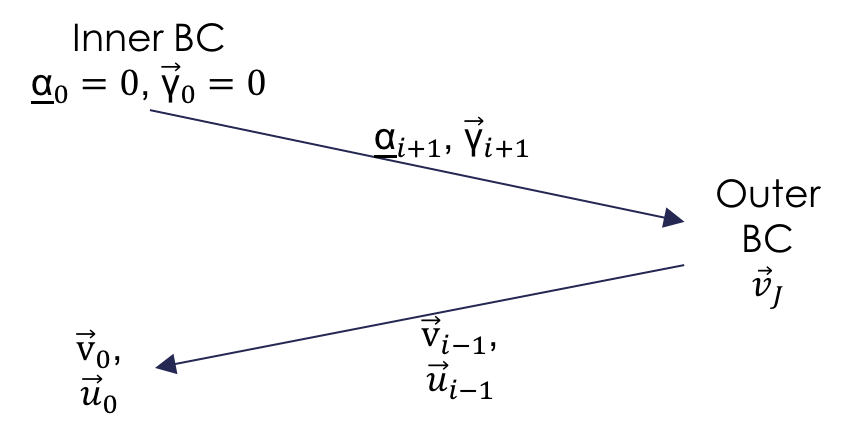
\includegraphics[width = 0.5 \textwidth]{figures/Overview.png}
\caption{A diagrammatic overview of the Henyey method, showing what is being evaluated at each stage of the code.  The arrows represent the two recurrence relations, with the inwards arrow progressively calculating the solution as it works back towards the centre of the grid.}
\label{fig:overview}
\end{center}
\end{figure}


This code was built from scratch, and tested extensively in various situations, particularly assessing the differences between analytically equivalent expressions of the recurrence relations and the differences between different applications of the boundary conditions.  The numerical components were also extensively tested, including ensuring the accuracy of matrix and vector manipulation, particularly matrix inversion in the case of small determinants; a structure to deal with the manipulation of complex numbers was built and tested; and a method of interpolation of input data was built, such that the maximum cell size could be precisely controlled and varied across the grid.  These were used to solve a variety of different equations, ranging from simple algebraic equations up to the complex differential equations which are used to solve the stellar oscillation equations.







\section{Implementing the equations}  \label{Implement}

This section discusses the practical side of the implementation of the stellar oscillation equations, including the problems associated with that, and how they were addressed and overcome.





\subsection{Discretisation}   \label{Implement:Disc}

The code cannot work directly with analytical equations, so the equations must be expressed in a discretised form, as a function of variables defined at distinct points on the numerical grid.  This must be done in such a manner as to minimise the loss of accuracy introduced by this process.

The variables are split into two different types: cell-centre variables, defined at the centre of the cell; and cell-face variables, defined at the outer edge of the cell.  $\vec{u}$ contains cell-face variables, and $\vec{v}$ contains cell-centre variables.  This is shown in figure \ref{fig:structure}.


\begin{figure}
\begin{center}
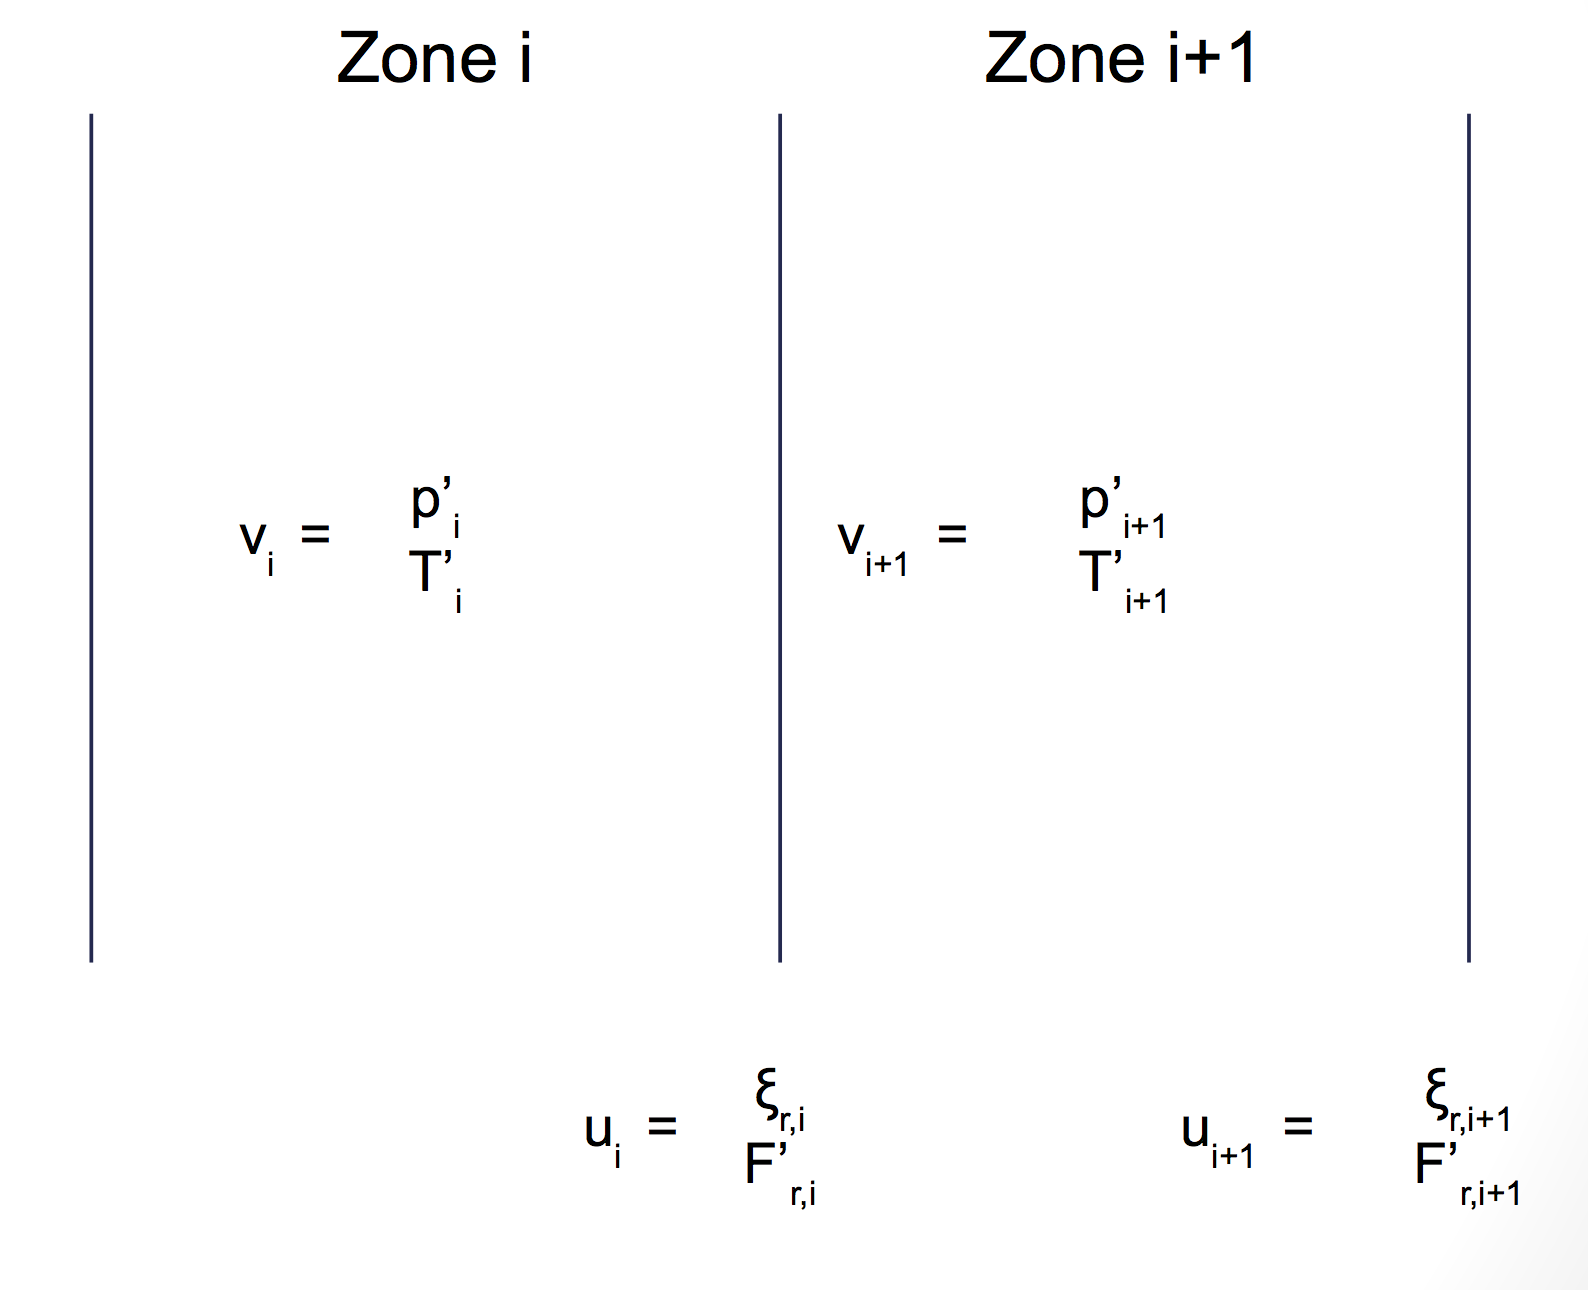
\includegraphics[width = 0.5 \textwidth]{figures/structure.png}
\caption{A representation of two adjacent cells, $i$ and $i+1$, showing the staggered variables.  $\vec{u}_{i}$ is defined at the outer surface of cell $i$, whilst $\vec{v}_{i}$ is defined at the midpoint of cell $i$.}
\label{fig:structure}
\end{center}
\end{figure}


\begin{figure}
\begin{center}
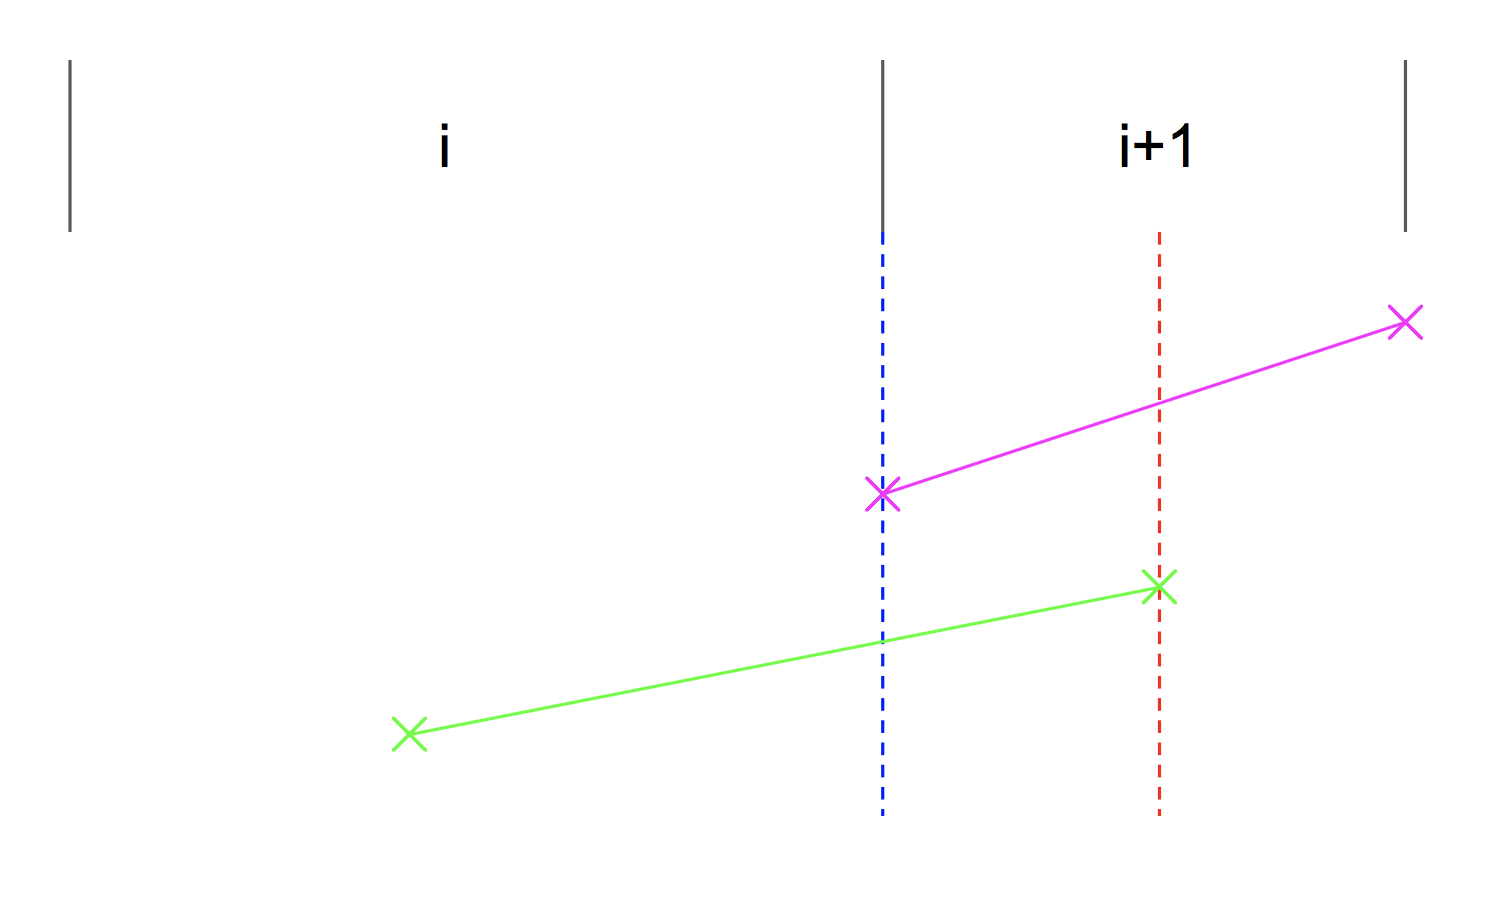
\includegraphics[width = 0.5 \textwidth]{figures/discretisation.png}
\caption{A representation of two adjacent cells, $i$ and $i+1$, showing the interpolation of variables.  The pink crosses represent a cell-face variable, such as $\xi_{r}$, whilst the green crosses represent a cell-centre variable, such as $p'$.  The red dashed line shows the location at which equations \ref{eq:cont_osc_dim2} and \ref{eq:ent_osc_dim2}, and therefore equation \ref{eq:ACD}, are evaluated.  The pink line connecting the cell-face variables shows that, at the location of the red dashed line, the cell-face variables must be interpolated, whereas the green cross sitting exactly on the line shows that the cell-centre variable is already defined at the required location.  The blue dashed line shows the location at which equations \ref{eq:flux_osc_dim2} and \ref{eq:mom_osc_dim2}, and therefore equation \ref{eq:EFH}, are evaluated.  Similarly, the pink cross sat on the dashed line shows that the cell-face variables are defined at the required location, whereas the green line shows that the cell-centre variables must be appropriately interpolated in order to minimise inaccuracy in the equations.  Note that the unequal cell sizes requires that this interpolation must be an unevenly weighted average.}
\label{fig:discretisation}
\end{center}
\end{figure}


For the Henyey method to work, we must express the equations that we are solving (equations \ref{eq:cont_osc_dim2} to \ref{eq:mom_osc_dim2}) in terms of variables in cells $k$ and $k+1$.  To do this precisely, the location at which the equations are evaluated must be carefully considered.  Figure \ref{fig:discretisation} shows how this is done.  In order for this interpolation and the derivatives to be accurate, a sufficiently fine grid must be used, such that the linear approximation is valid.







\subsection{Input data}   \label{Implement:Input}

The equations \ref{eq:cont_osc_dim2} to \ref{eq:mom_osc_dim2} solve for small perturbations to an equilibrium model.  In order to do this, the equilibrium state of the star must be accurately known.  

To do this, I use Modules for Experiments in Stellar Astrophysics (MESA) \cite{Paxton2011} to generate $1$D, spherically symmetric models of stars.  This enables me to match the observed parameters of any system that I may seek to recreate, varying the mass, metallicity, and age of the star, amongst other things.  There is, however, some exploration required with this process, as MESA does not retrofit parameters such as brightness or surface temperature, but rather evolves the star from the initial properties.

This code outputs the equilibrium state on a grid, which defines the basic grid upon which I must solve my equations.  In order to maintain accuracy in my solution, the grid must be sufficiently fine to accurately interpolate, and also able to reliably capture any highly oscillatory behaviour in the solution (that is expected to be the radiative regions, where solutions are expected to be oscillatory, whereas they are expected to be evanescent in convective zones).  Unhelpfully, the areas in which the solution is oscillatory are areas in which MESA deems the structure to be simple, and therefore produces a low-resolution grid.

To increase the resolution, the large MESA cells must be split into smaller cells, and the data interpolated to find the appropriate values on this new grid.  This could lead to a variety of problems, including needing to be careful to strictly interpolate rather than extrapolate, and the potential for artificially large derivatives, and therefore requires careful treatment, but these problems should be avoided if the MESA grid is sufficiently fine for linear interpolation to be valid.






\subsection{Other considerations}   \label{Implement:Other}

I will outline some other problems in the implementation of the Henyey code to solve the oscillation equations here, particularly focussing on how they were overcome, or worked around.


In choosing the form of the recurrence relations used in the Henyey code, multiple different expressions for analytically equivalent versions were possible.  A major consideration was to ensure that inverting singular matrices (such as using $\underline{\alpha}_{0}^{-1}$) was avoided, which limited the possible sensible range of expressions.  Even so, these different expressions were tested to discover which versions were most effective in solving the test equations, and how to express them using the fewest matrix manipulations.  For the outgoing recurrence relation, there was only one essential expression, and all the others were found to be exactly analytically equivalent.  For the returning recurrence relation, however, two genuinely distinct options are available.  Both cases were tested and their accuracy evaluated, and case I was selected to be used.  Further details can be found in appendix \ref{ap:Henyey}.


A major obstacle to achieving the required resolution was the limitation due to the size of the available RAM.  This is a result of the fact that the process to iterate from step $k+1$ to $k$ on the return journey requires information which was used to step from $k$ to $k+1$ on the outgoing journey.  As such, each step is not stand-alone, and a large amount of memory was being used in defining each matrix at each location in the star for the entirety of the calculation.  In order to improve this situation, I introduced some new arrays which would be used specifically to exactly what would be needed for the return journey, and only that information.  Using this, each matrix array need only contain the information for the step from $k$ to $k+1$ at the time that that outward step is being evaluated, as the required information for the step from $k+1$ to $k$ on the return journey would be evaluated at that point and saved, then the matrices would be re-evaluated for the next outward step.  This introduces a few arrays of dimension $2 \times 2 \times J$, but also cuts down many arrays from the previously required $2 \times 2 \times J$ to $2 \times 2 \times 2$.  This solution does still hit another limit, however, as there are still some matrices which grow linearly with the resolution, so the RAM limitation is still in place, but at a suitable resolution (that is, $J = 20000$ rather than $J = 1000$).  Also, as the resolution is controlled as a function of position in the star, the limited number of cells can be distributed such that the highest resolution is where the need is greatest, although this is not an automatic process, but must be managed manually.







\section{Output} \label{Output}

In order to ensure that the code and equations are all correct, work from a previous paper (Terquem \textit{et al}, 1998, figure 1) has been reproduced and the output has been compared.  The previous work used a shooting method, and treated the non-adiabatic case slightly differently, but good agreement has been found between the paper's result and my own, which can be seen in figure \ref{fig:non-ad}.  Some particular differences to note are the following: the precise form of spatial oscillations in the core varies depending on the exact parameters used in the solution (which will be explored in the following paragraphs), and the behaviour at the very surface (that is, the last $\sim 0.1 \%$ of the star's radius) is significantly different, although this is due to the thin outermost radiative layer of the star, and is not thought to be a problem with the Henyey method's application in this case.



\begin{sidewaysfigure}[htbp]
\begin{center}
\begin{subfigure}{0.5\textheight}
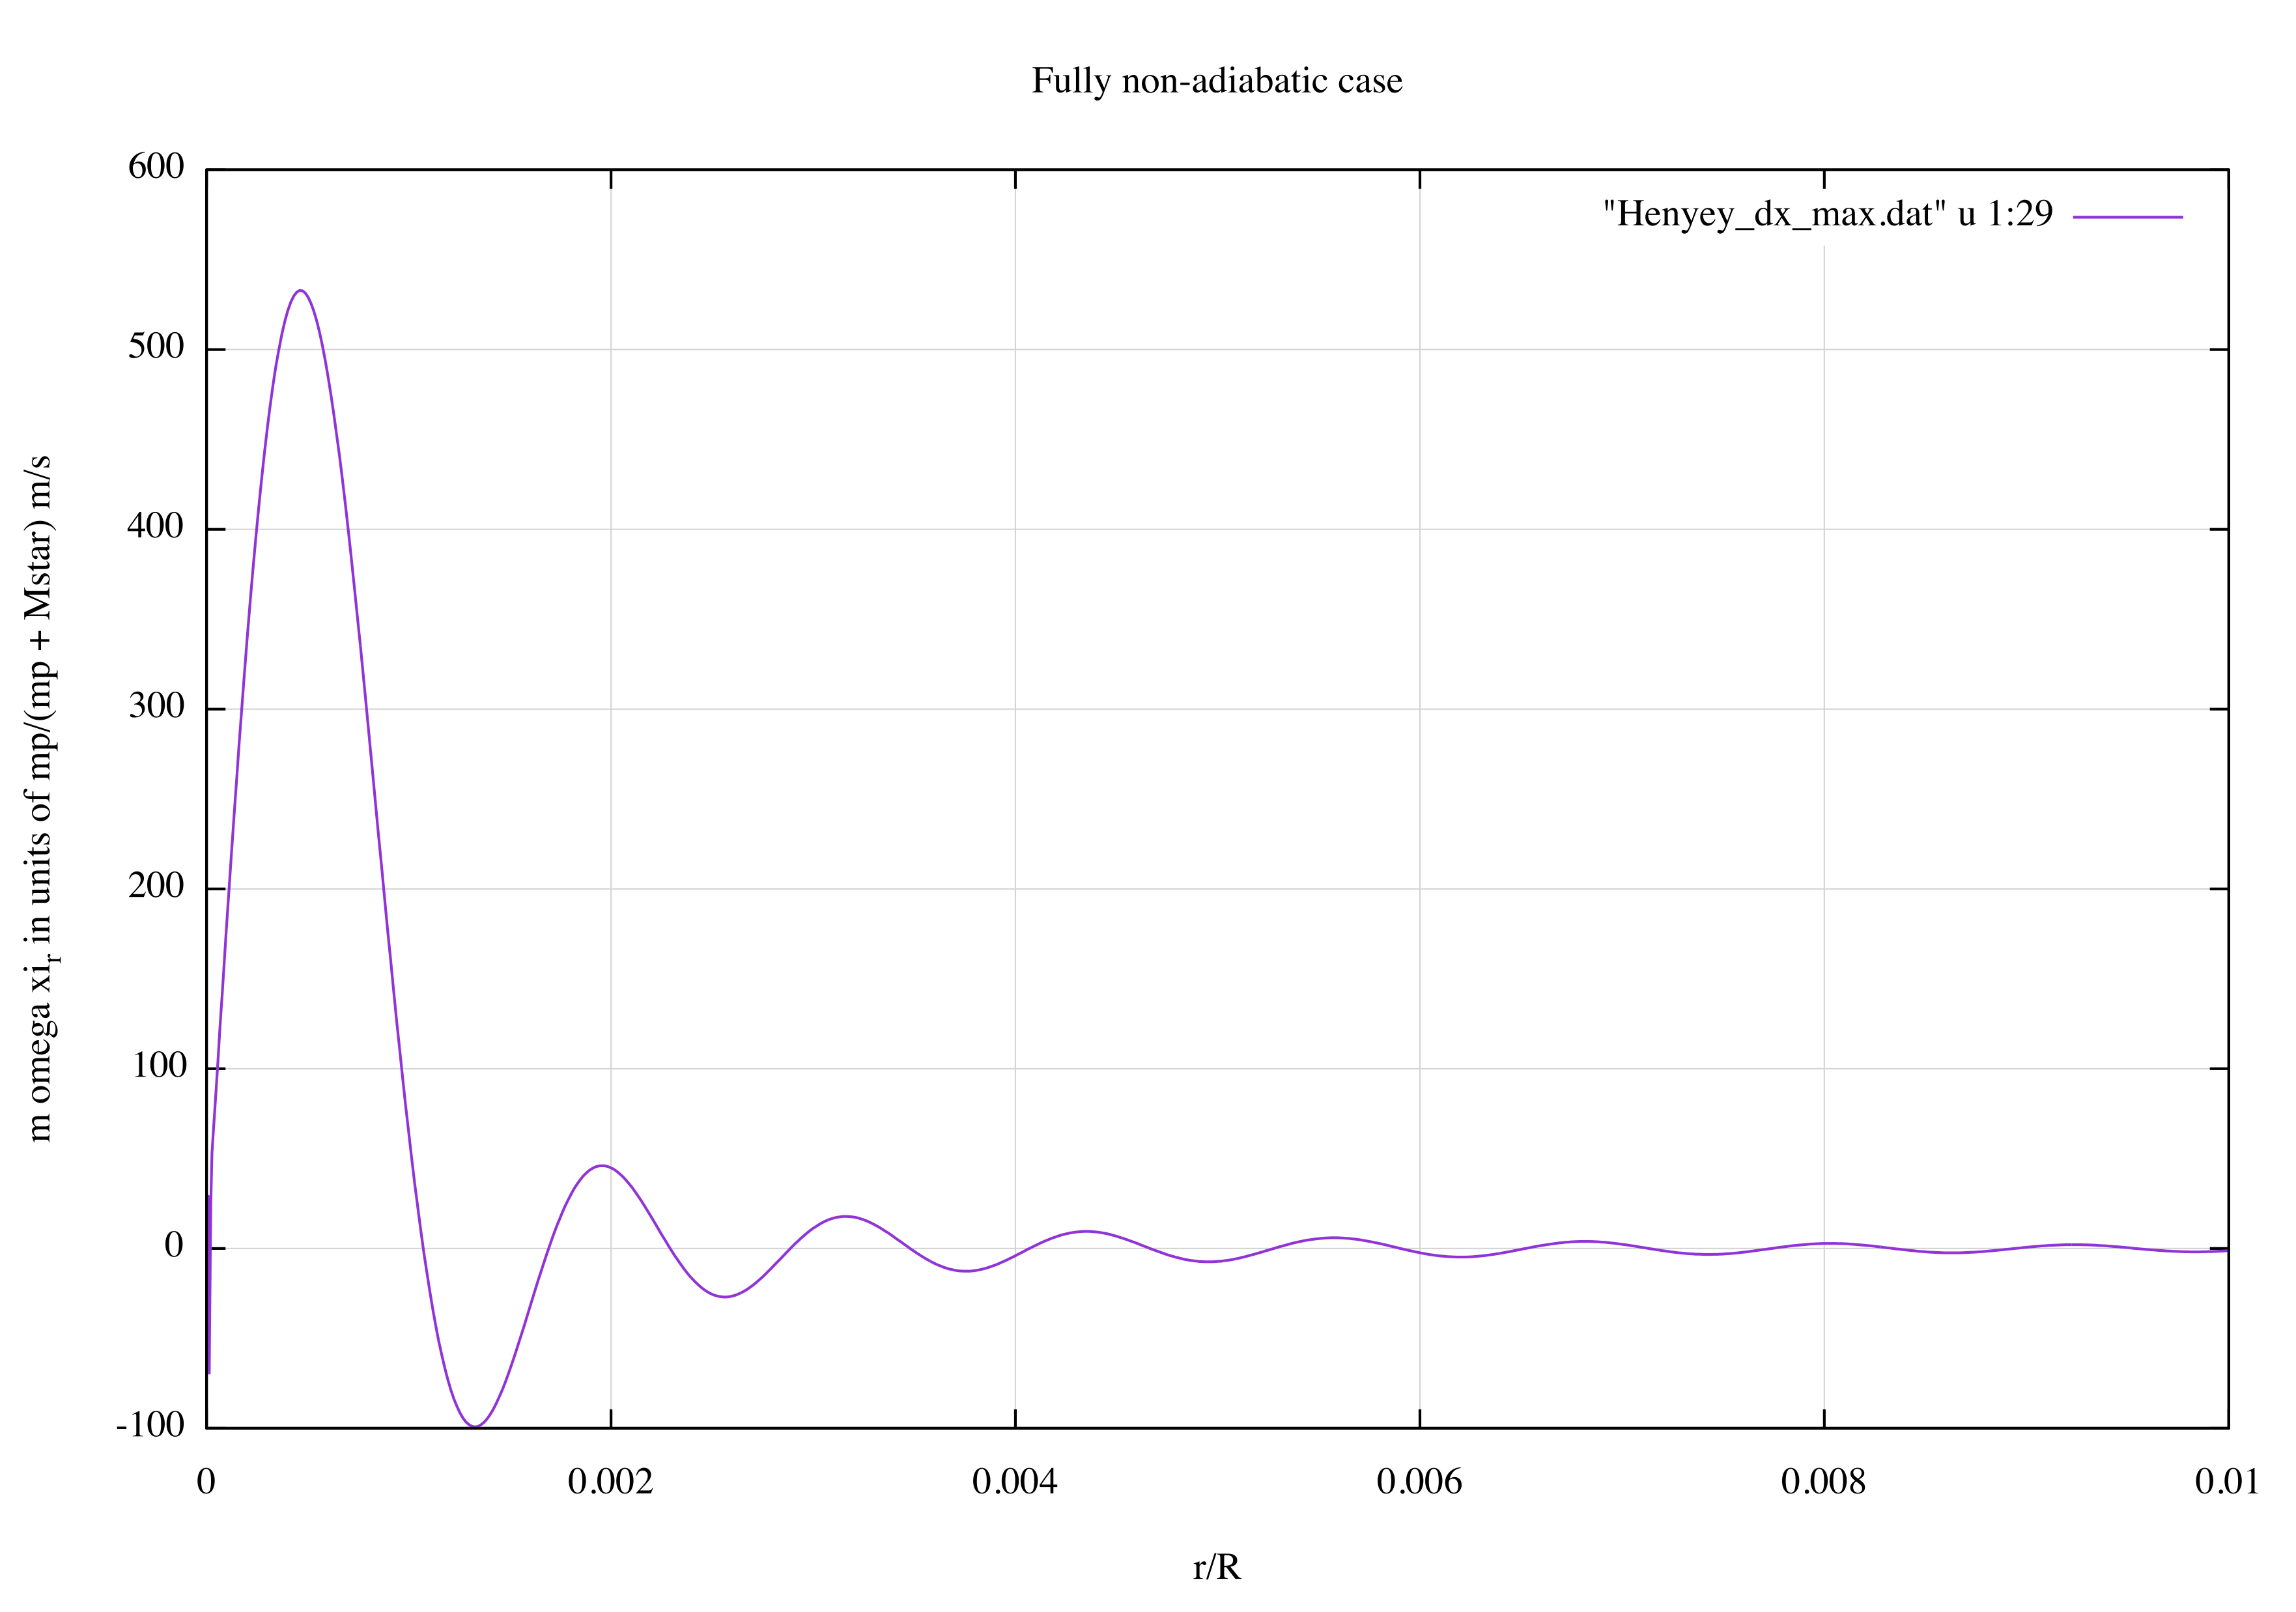
\includegraphics[width = \textwidth]{figures/xi_r_section1_non-ad.png}
\end{subfigure}
~
\begin{subfigure}{0.5\textheight}
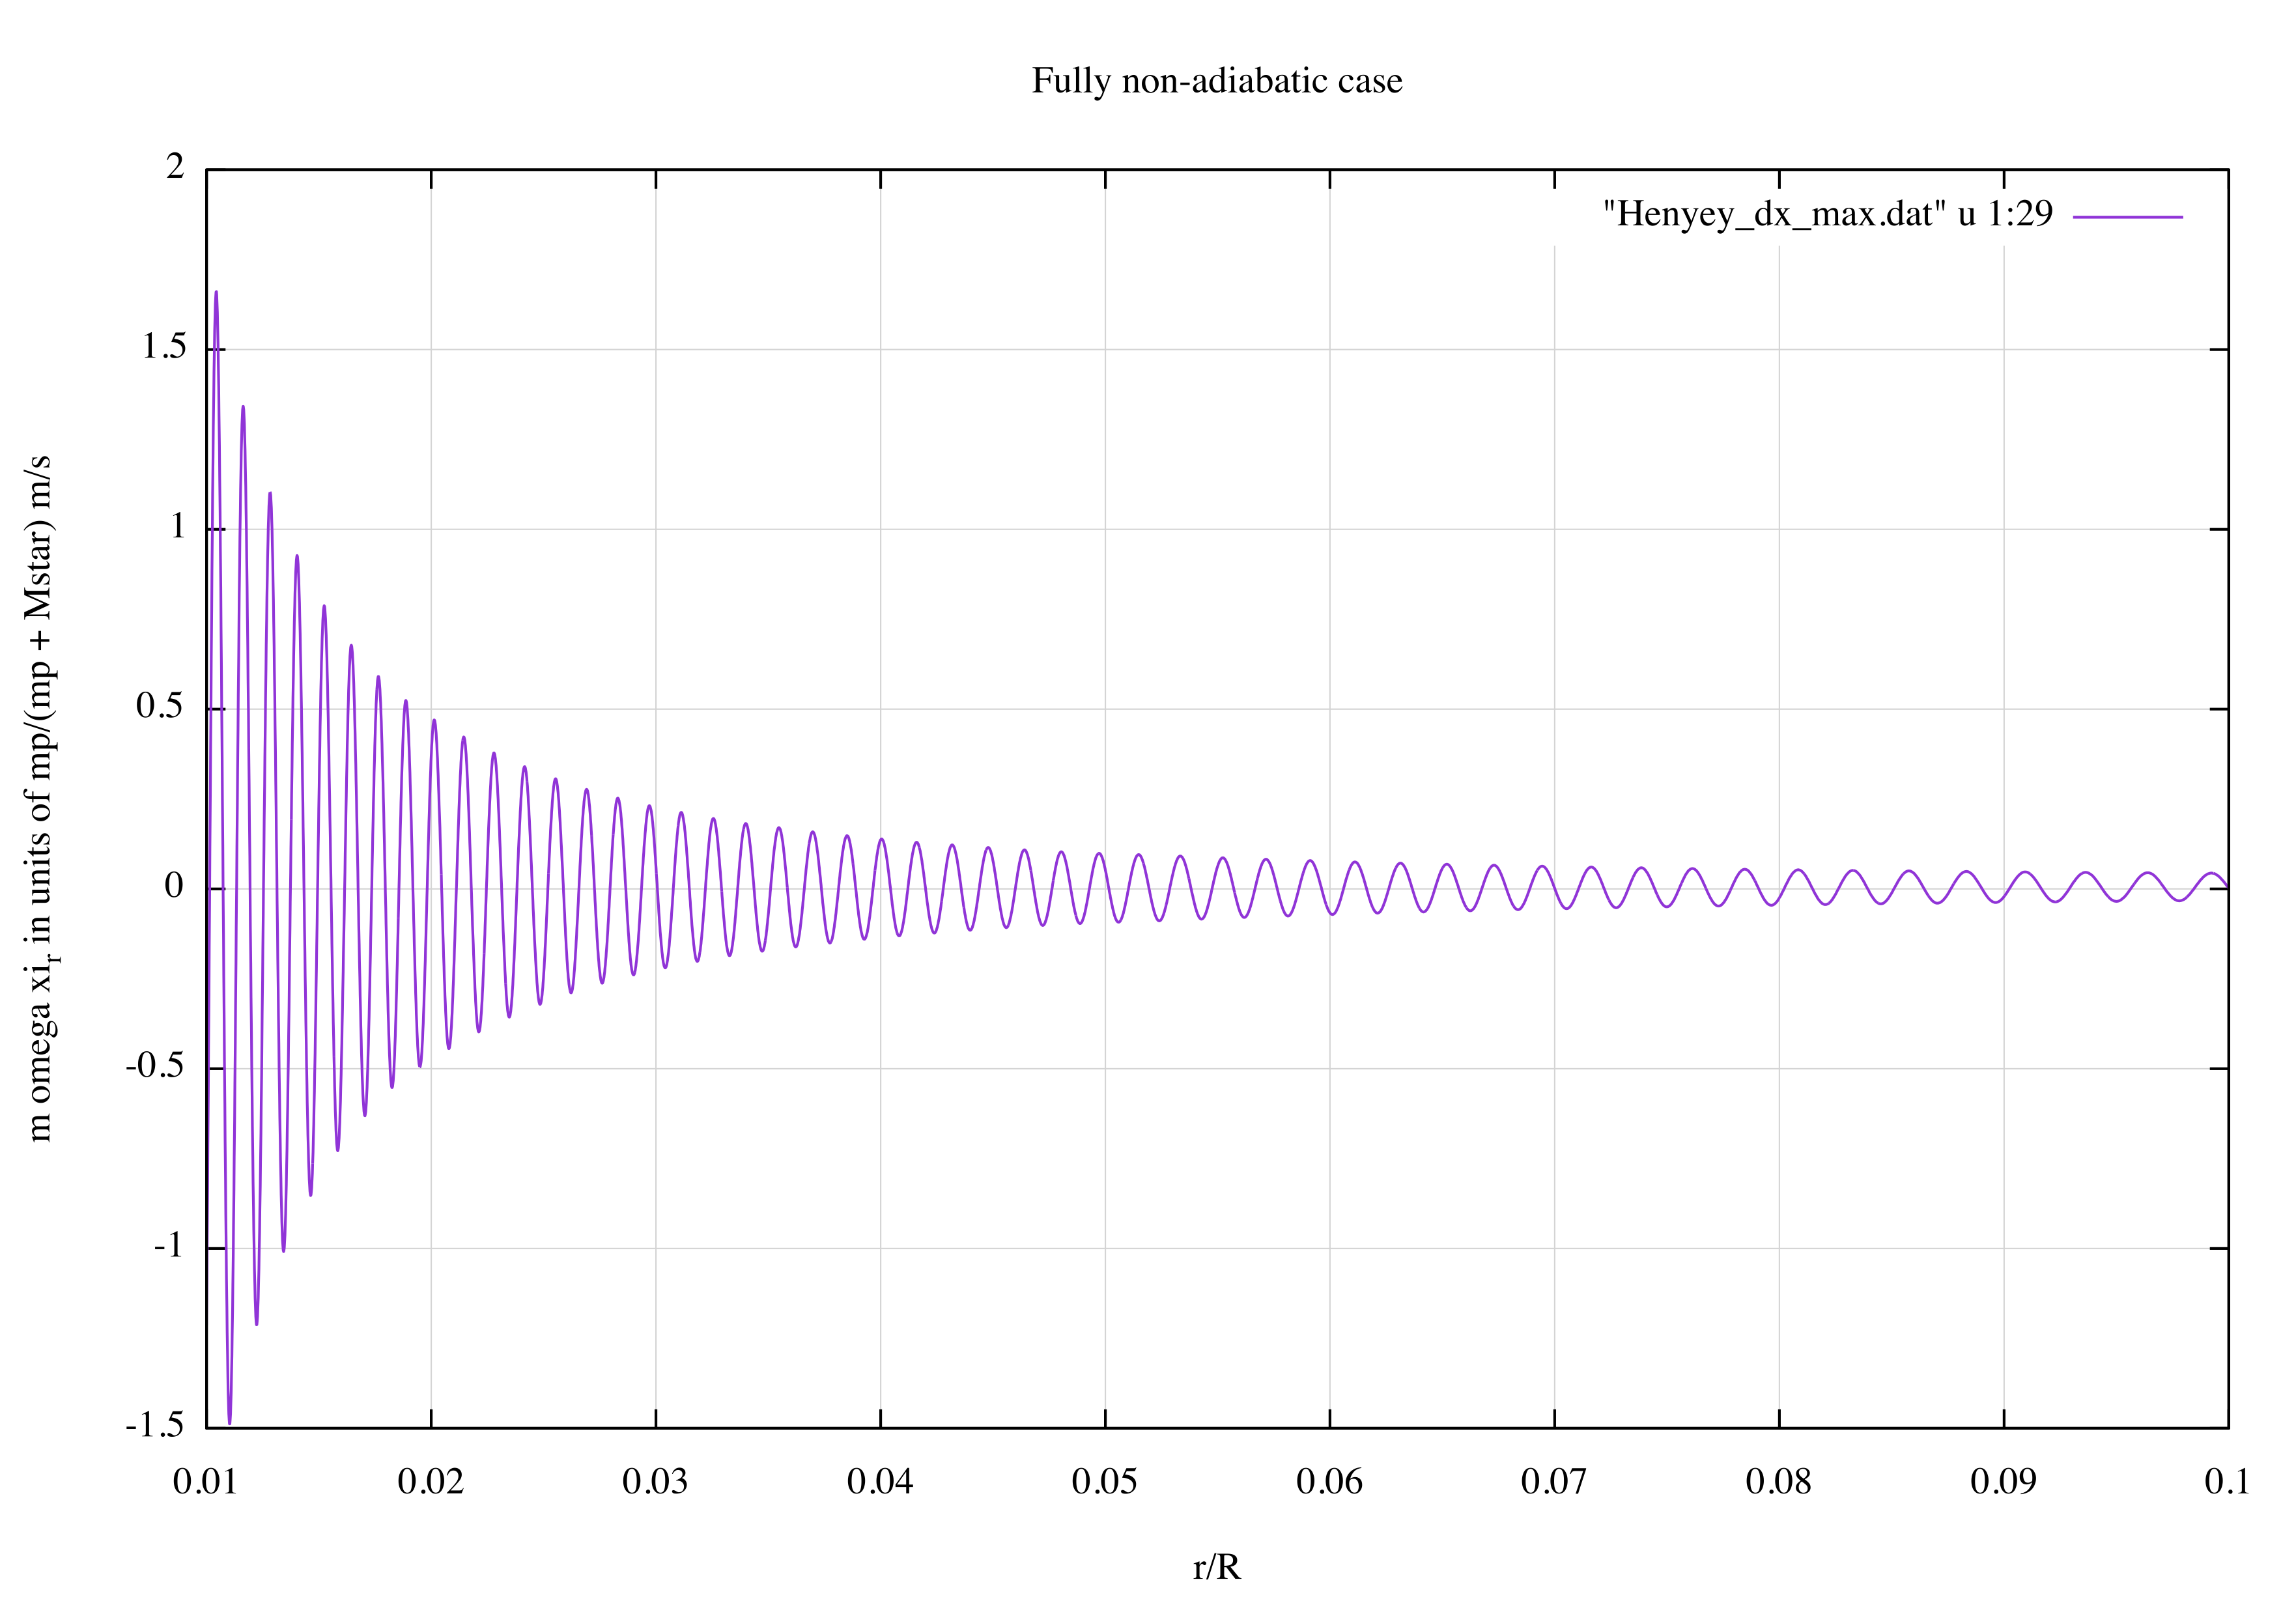
\includegraphics[width = \textwidth]{figures/xi_r_section2_non-ad.png}
\end{subfigure}

\begin{subfigure}{0.5\textheight}
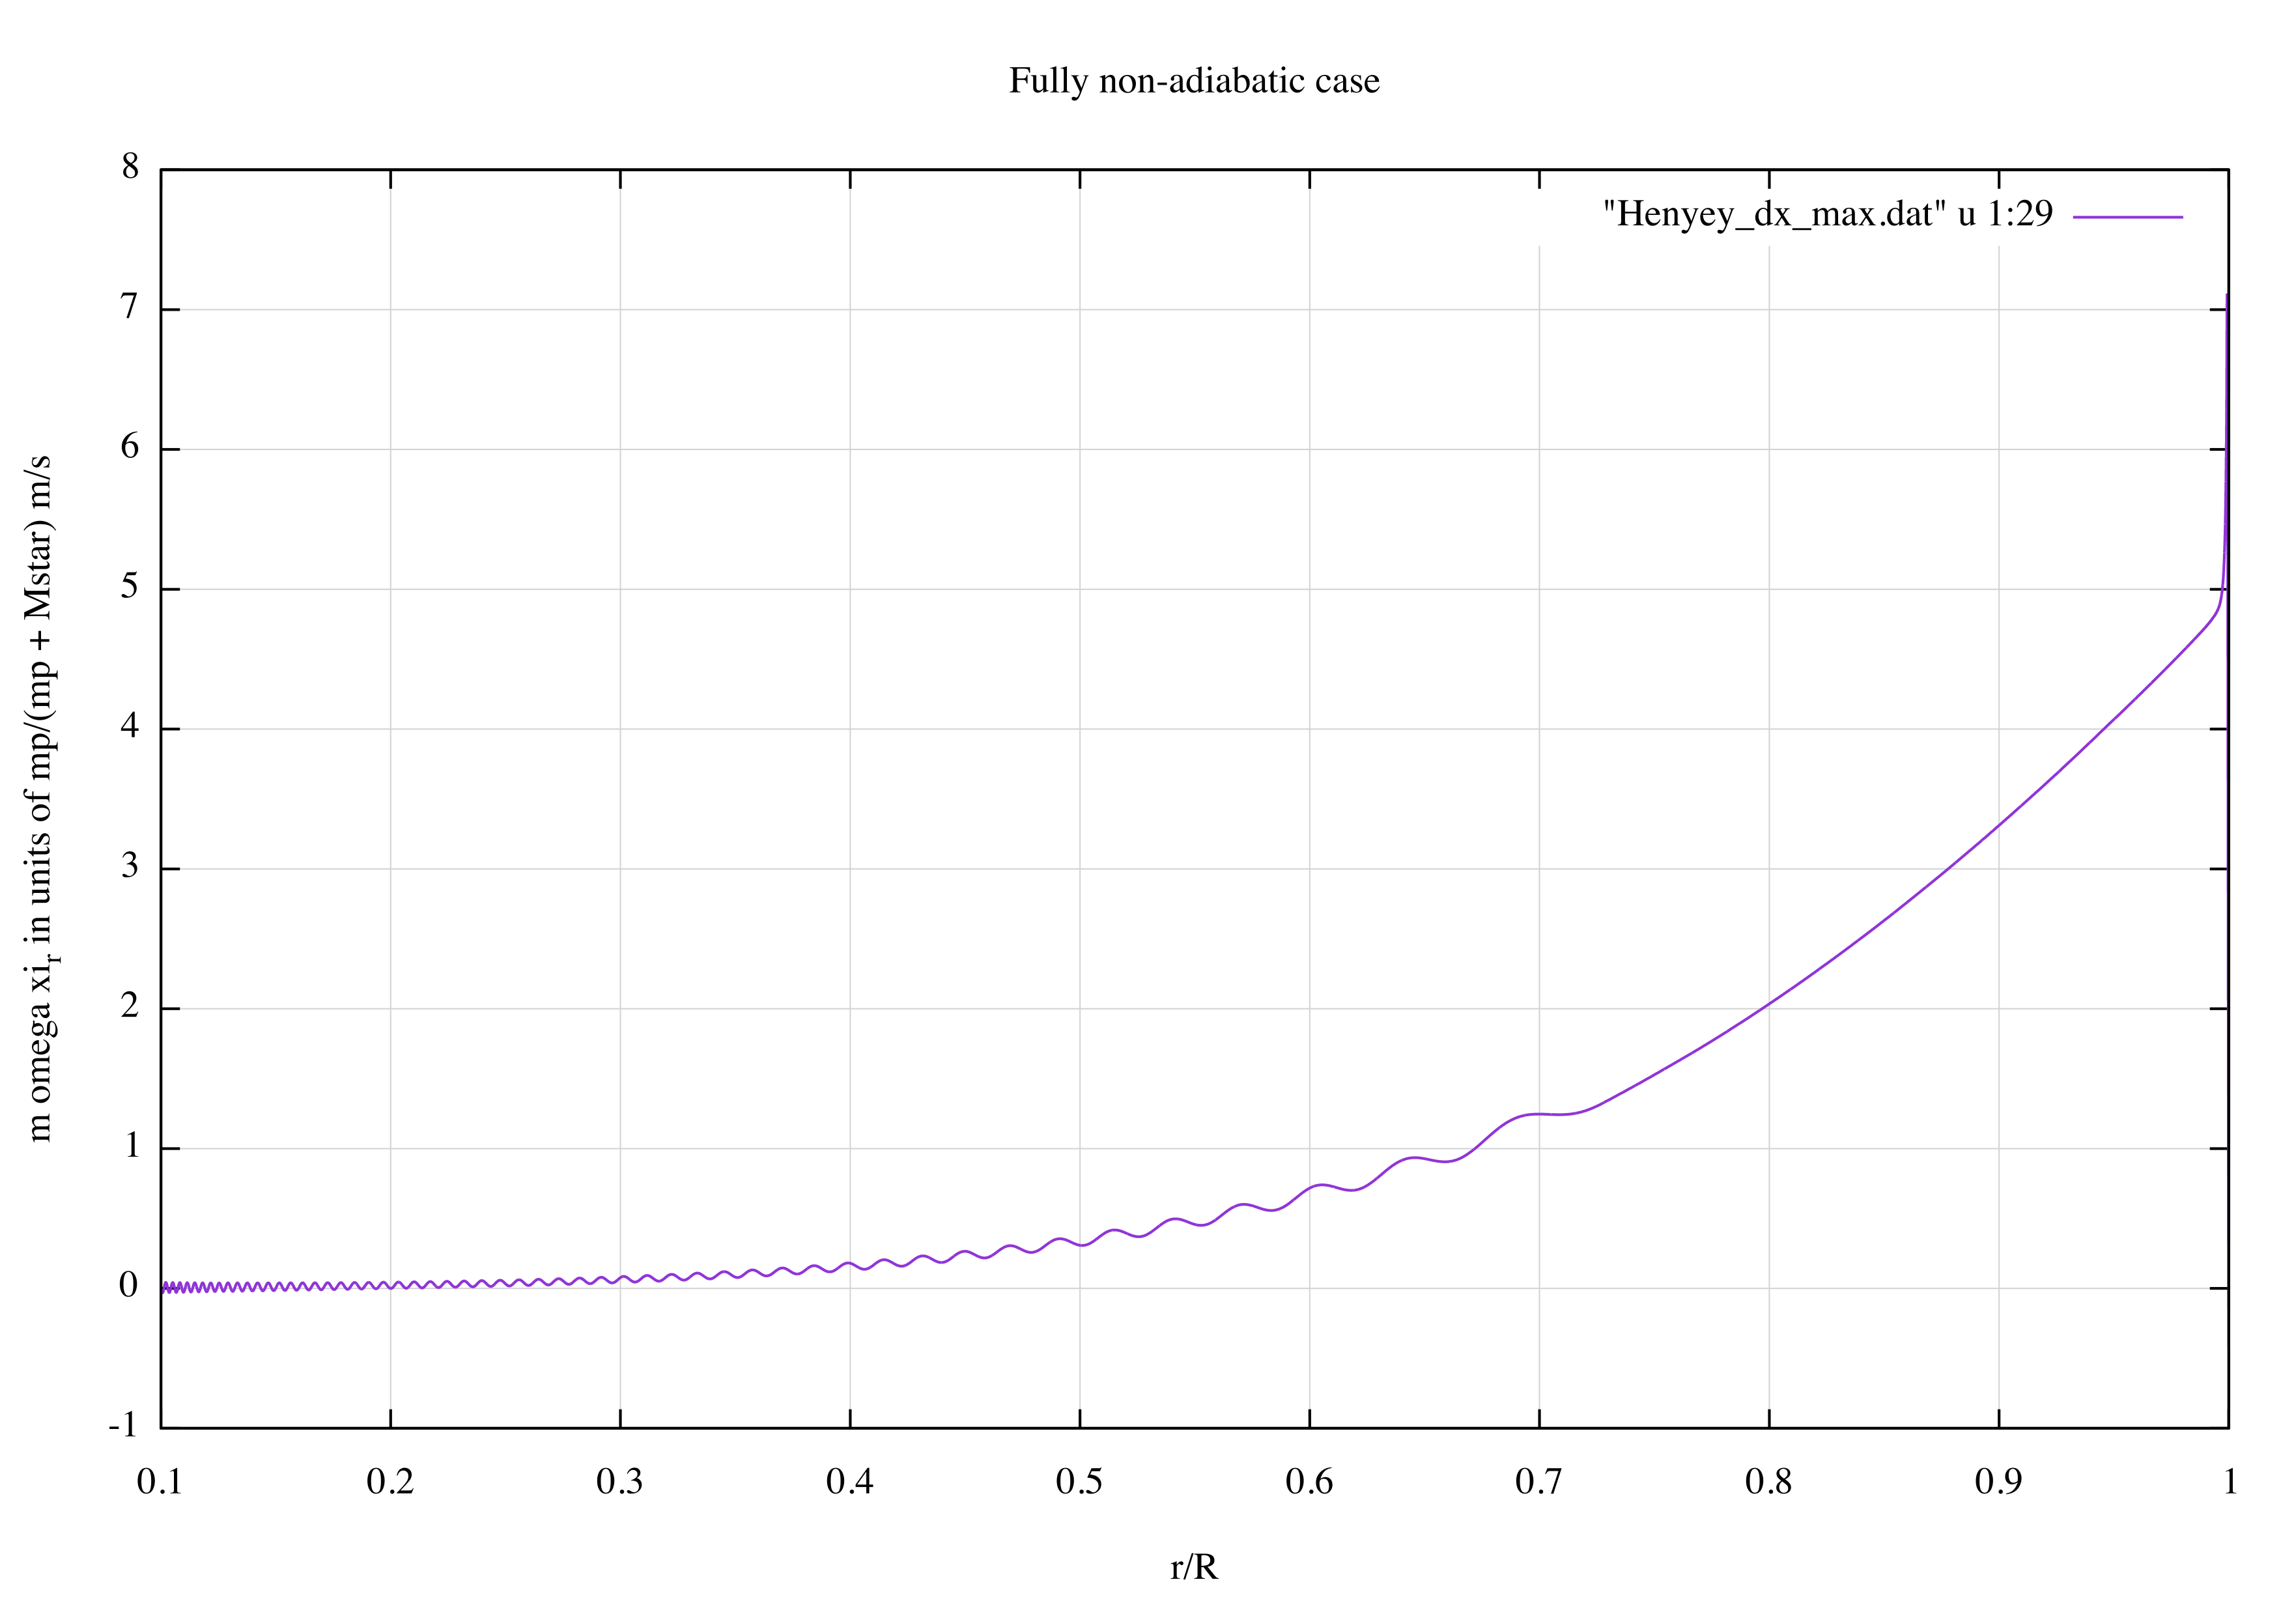
\includegraphics[width = \textwidth]{figures/xi_r_section3_non-ad.png}
\end{subfigure}
~
\begin{subfigure}{0.5\textheight}
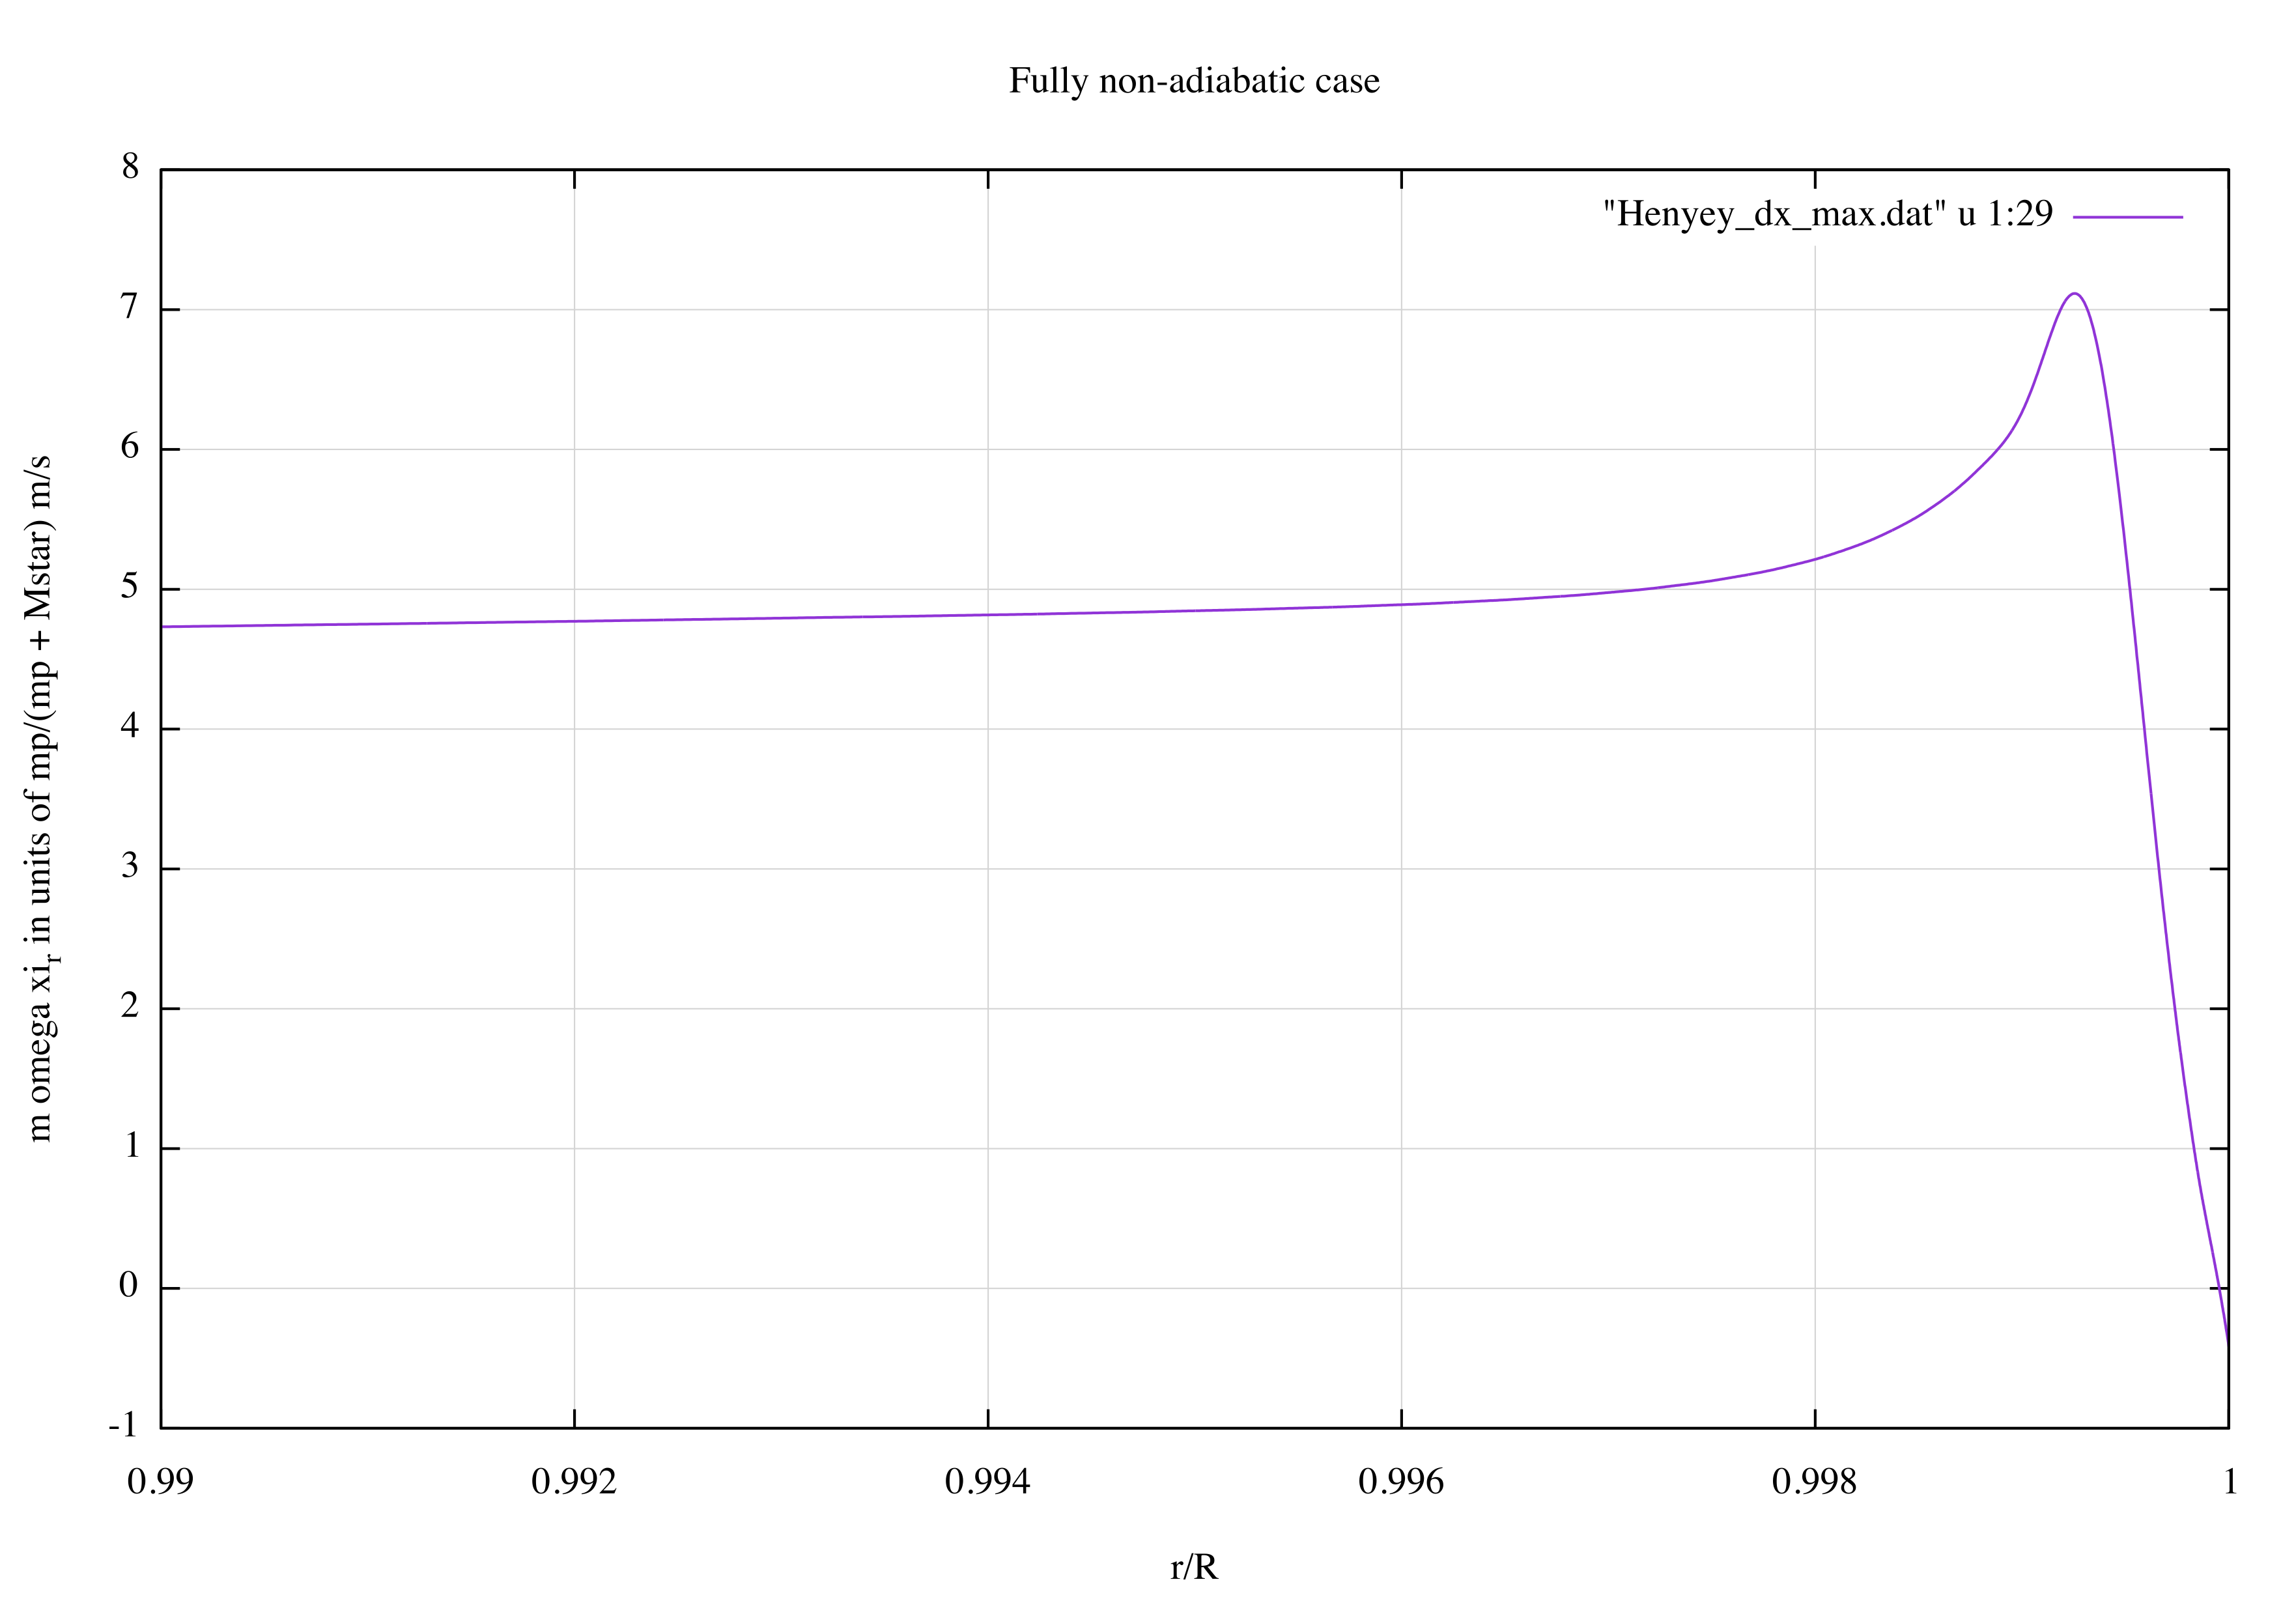
\includegraphics[width = \textwidth]{figures/xi_r_surface_non-ad.png}
\end{subfigure}

\caption{The full solution for the non-adiabatic case, showing the peak radial velocity (that is, $m \omega \xi_{r}$) in units of $\frac{m_{p}}{m_{p} + M_{*}}$ m s$^{-1}$, against the proportional radial distance from the centre.  Four segments have been shown, as the first three reproduce the graphs in Terquem \textit{et al}, 1998, and the fourth highlights the behaviour in the thin radiative layer at the star's surface.  As a rough guide, the y-axis is approximately in mm s$^{-1}$}
\label{fig:non-ad}
\end{center}
\end{sidewaysfigure}



To investigate some of the limitations of this solution, some of the parameters used in the solution were varied slightly, to investigate what effect this had in the different regions of the star.

Firstly, a purely physical parameter was varied by up to $1 \%$, the semi-major axis of the planet's orbit.  This would be expected to have a slight effect on the amplitude of the response throughout the star, as a more distant planetary companion would lead to a lessened tidal effect, but it would also slightly shift the frequency of the orbit, and would therefore be expected to alter the spatial frequency of oscillations within the star.  This effect can be seen in figure \ref{fig:Dvar}, where it is particularly notable that the amplitude of the spatial oscillations at the very centre varies hugely, from, effectively, $-300$ to $+500$ mm s$^{-1}$.  The overall trend, however of oscillations which grow towards the centre of the core is clearly maintained, as is the decrease in spatial frequency further from the core.  The transition to evanescent waves in the convective envelope (from $\frac{r}{R} \approx 0.7$) is consistent across the cases, and is very similar in amplitude (particularly given that the magnitude of the tidal potential varies as $D^{-3}$).  Overall, it seems that the observable behaviour is not particularly sensitive to small variations in $D$ for this case, and that the patterns of behaviour in each region are unaffected, but that one should be wary of drawing precise quantitative conclusions about the oscillations in the core.





\begin{sidewaysfigure}[htbp]
\begin{center}
\begin{subfigure}{0.5\textwidth}
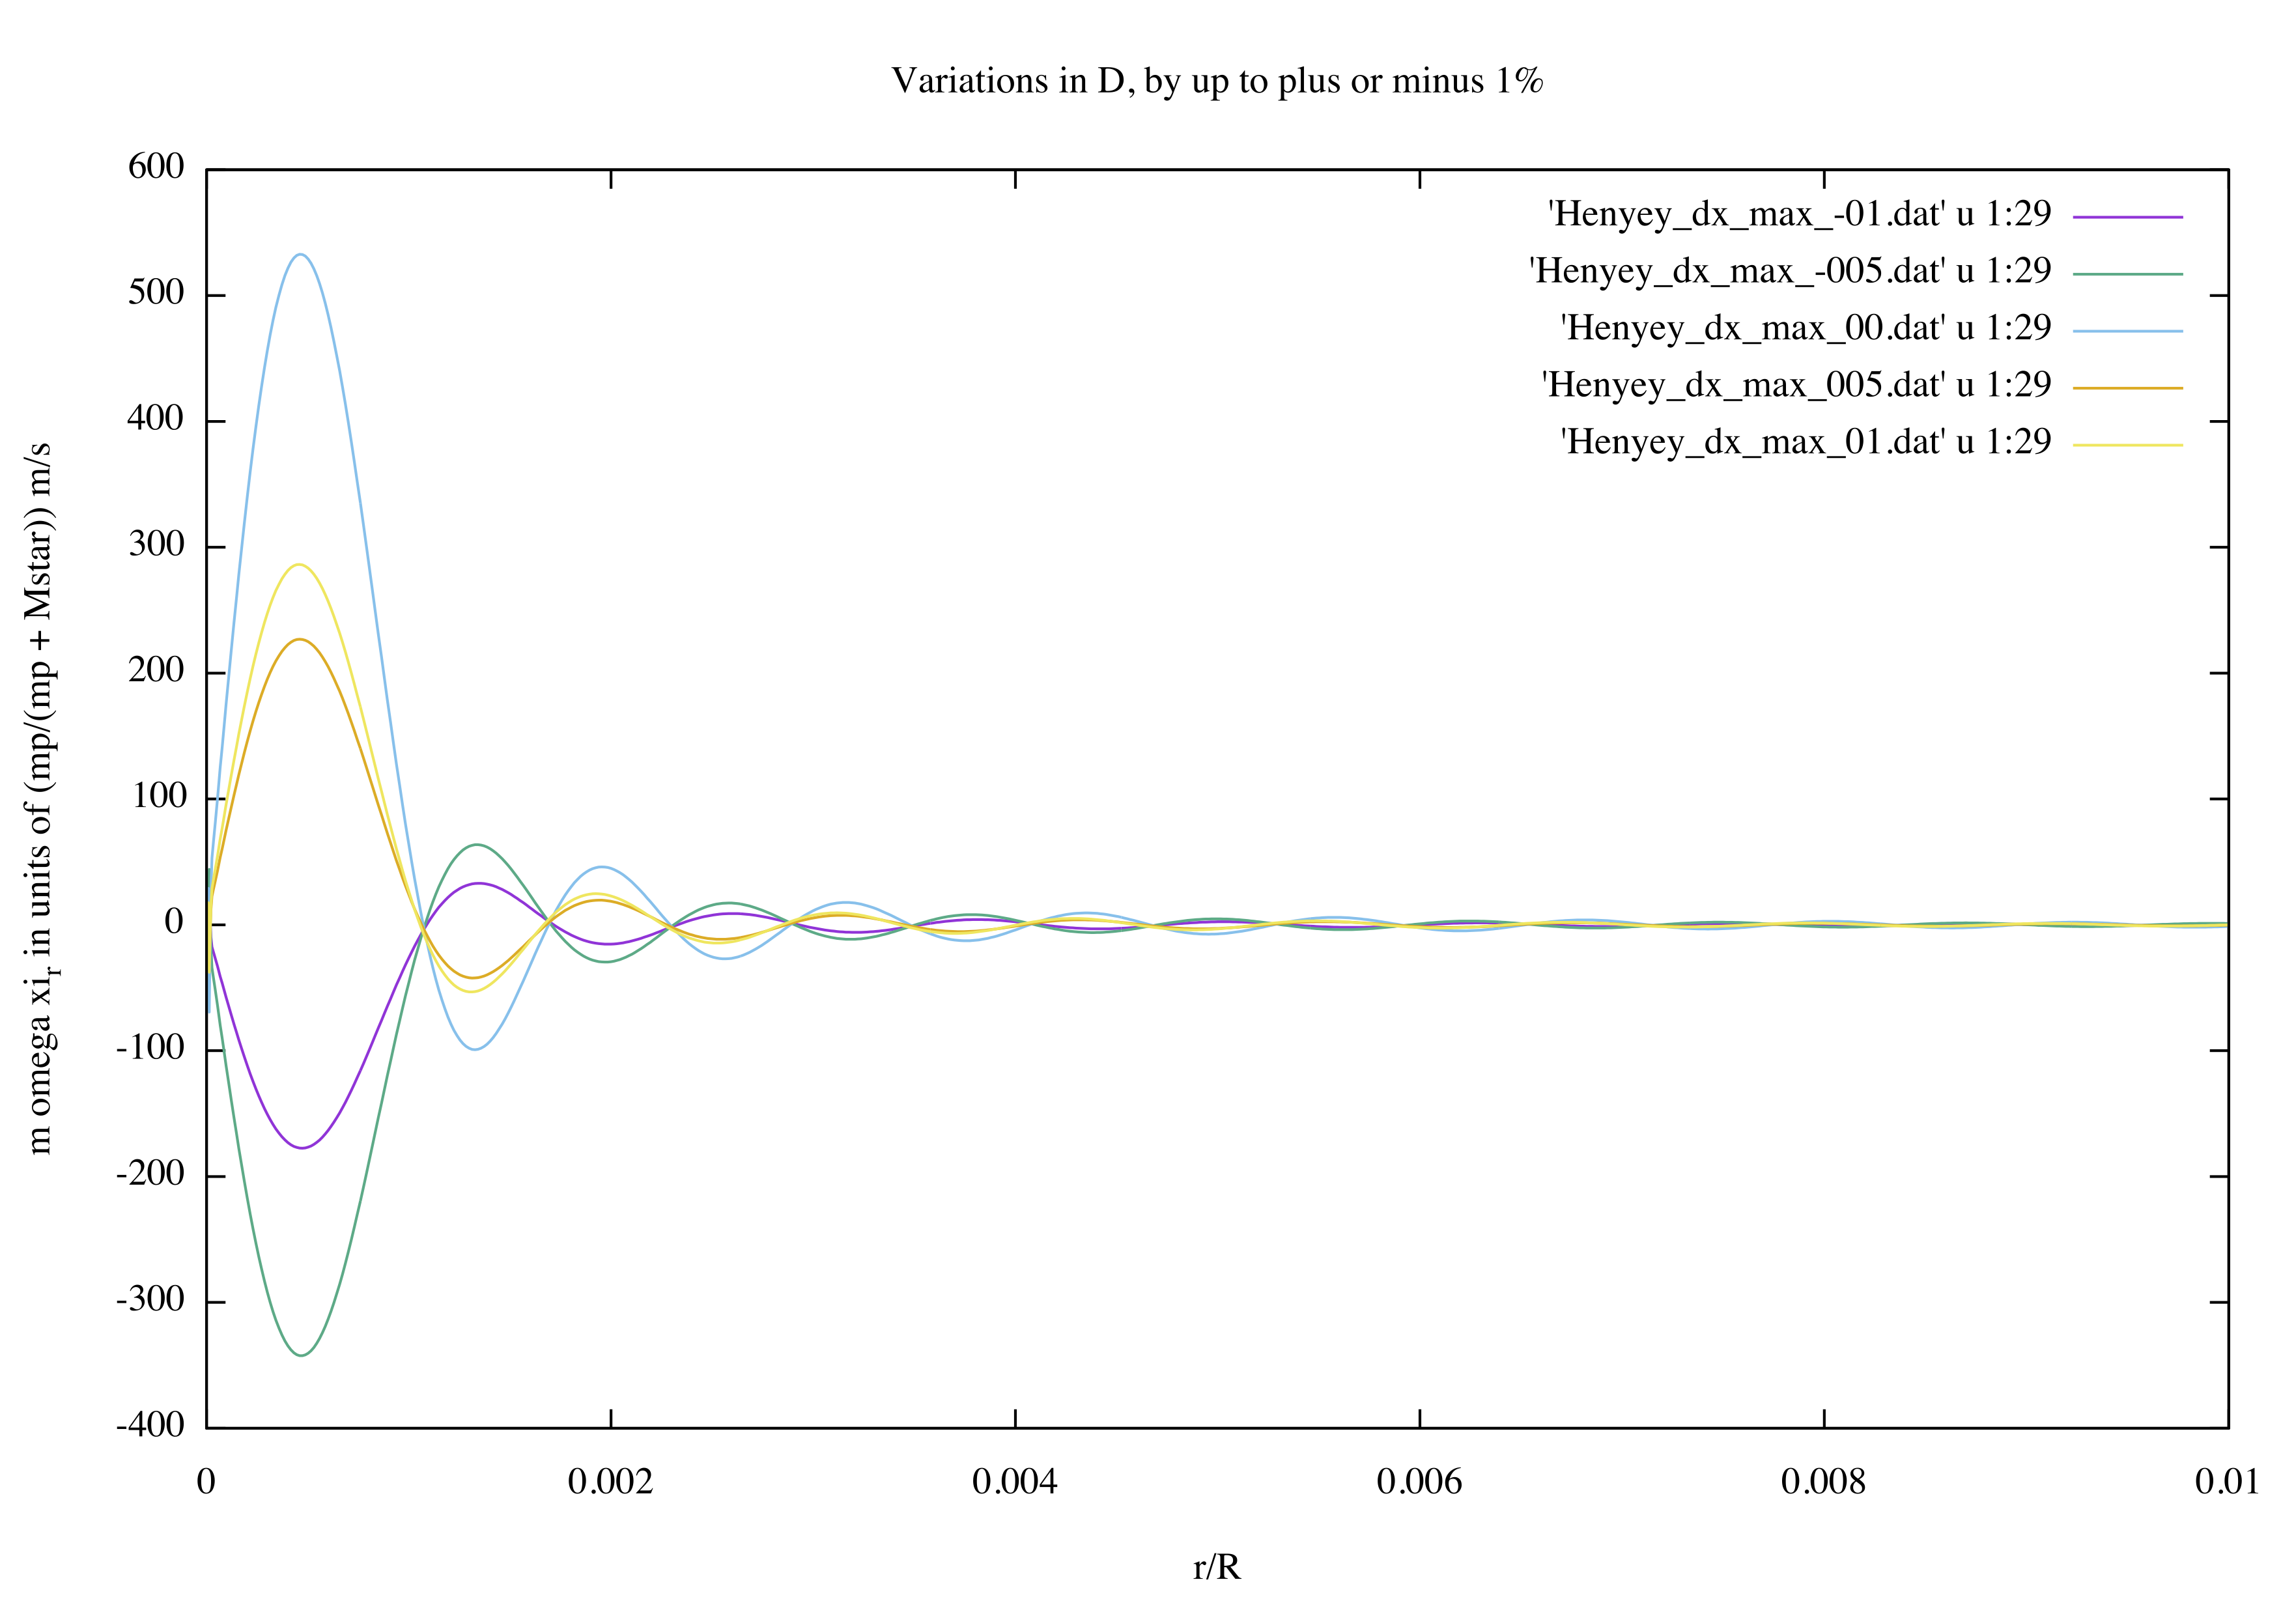
\includegraphics[width = \textwidth]{figures/xi_r_section1_Dvar.png}
\end{subfigure}
~
\begin{subfigure}{0.5\textwidth}
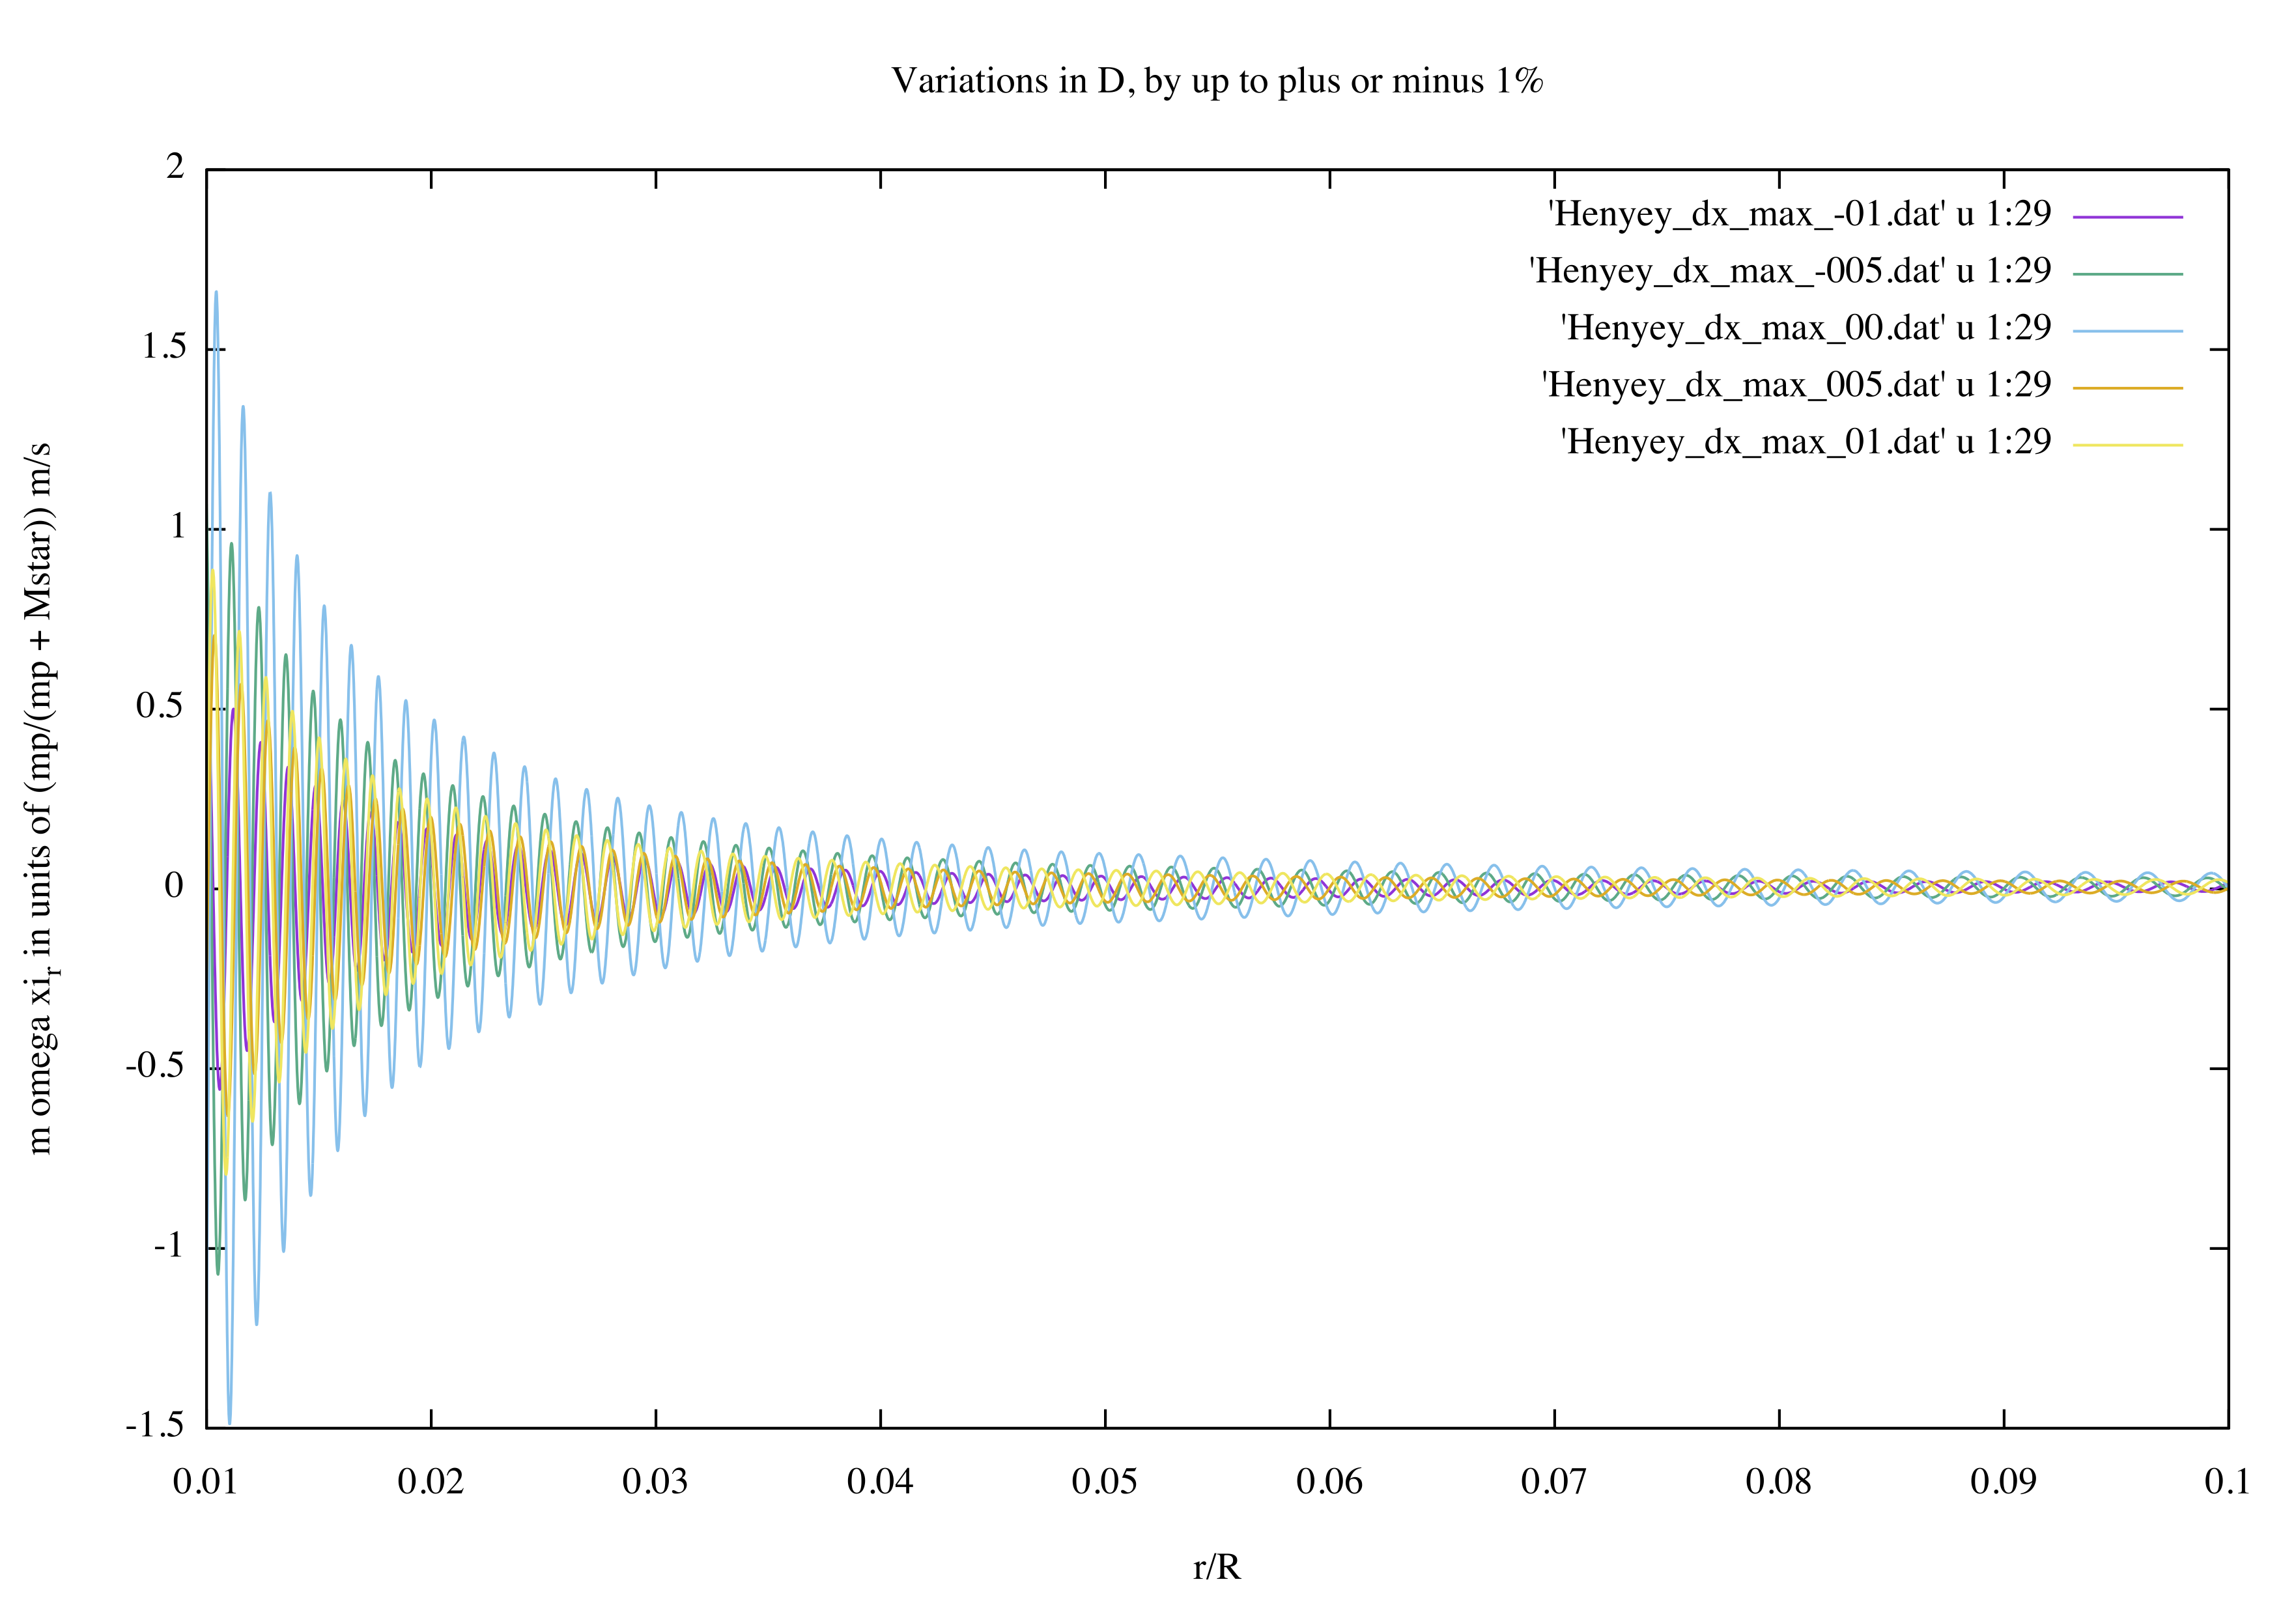
\includegraphics[width = \textwidth]{figures/xi_r_section2_Dvar.png}
\end{subfigure}

\begin{subfigure}{0.5\textwidth}
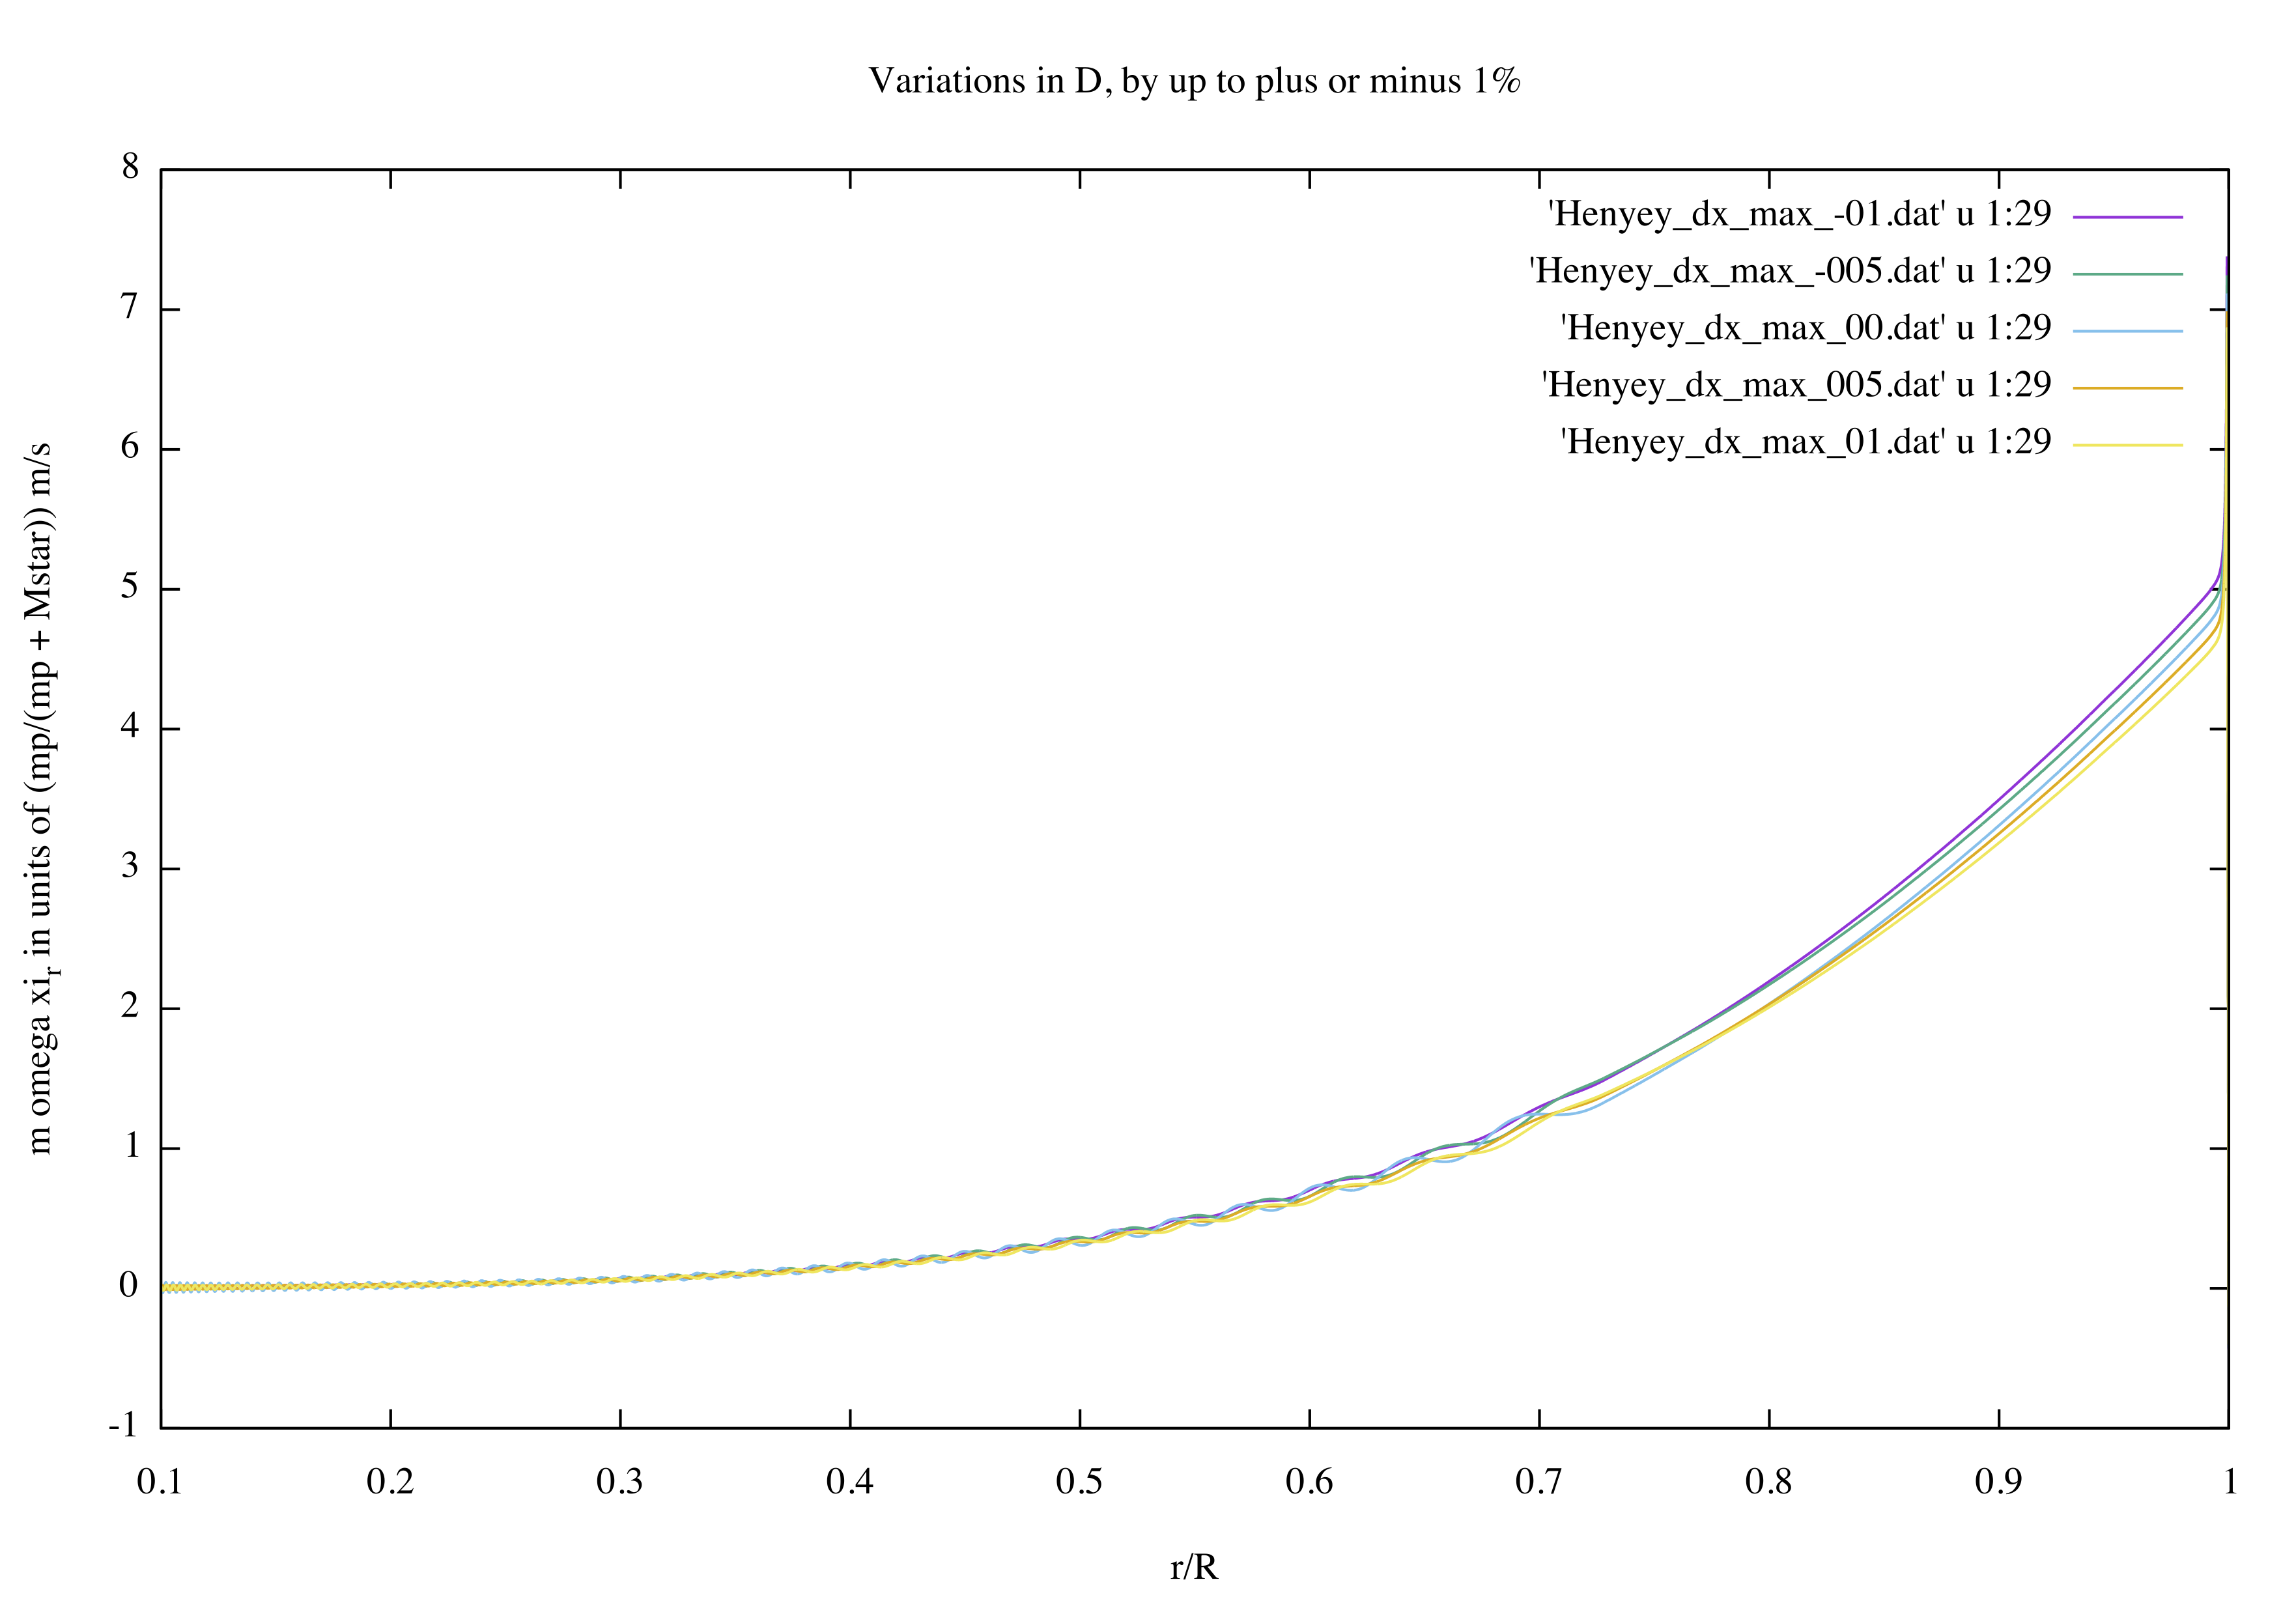
\includegraphics[width = \textwidth]{figures/xi_r_section3_Dvar.png}
\end{subfigure}
~
\begin{subfigure}{0.5\textwidth}
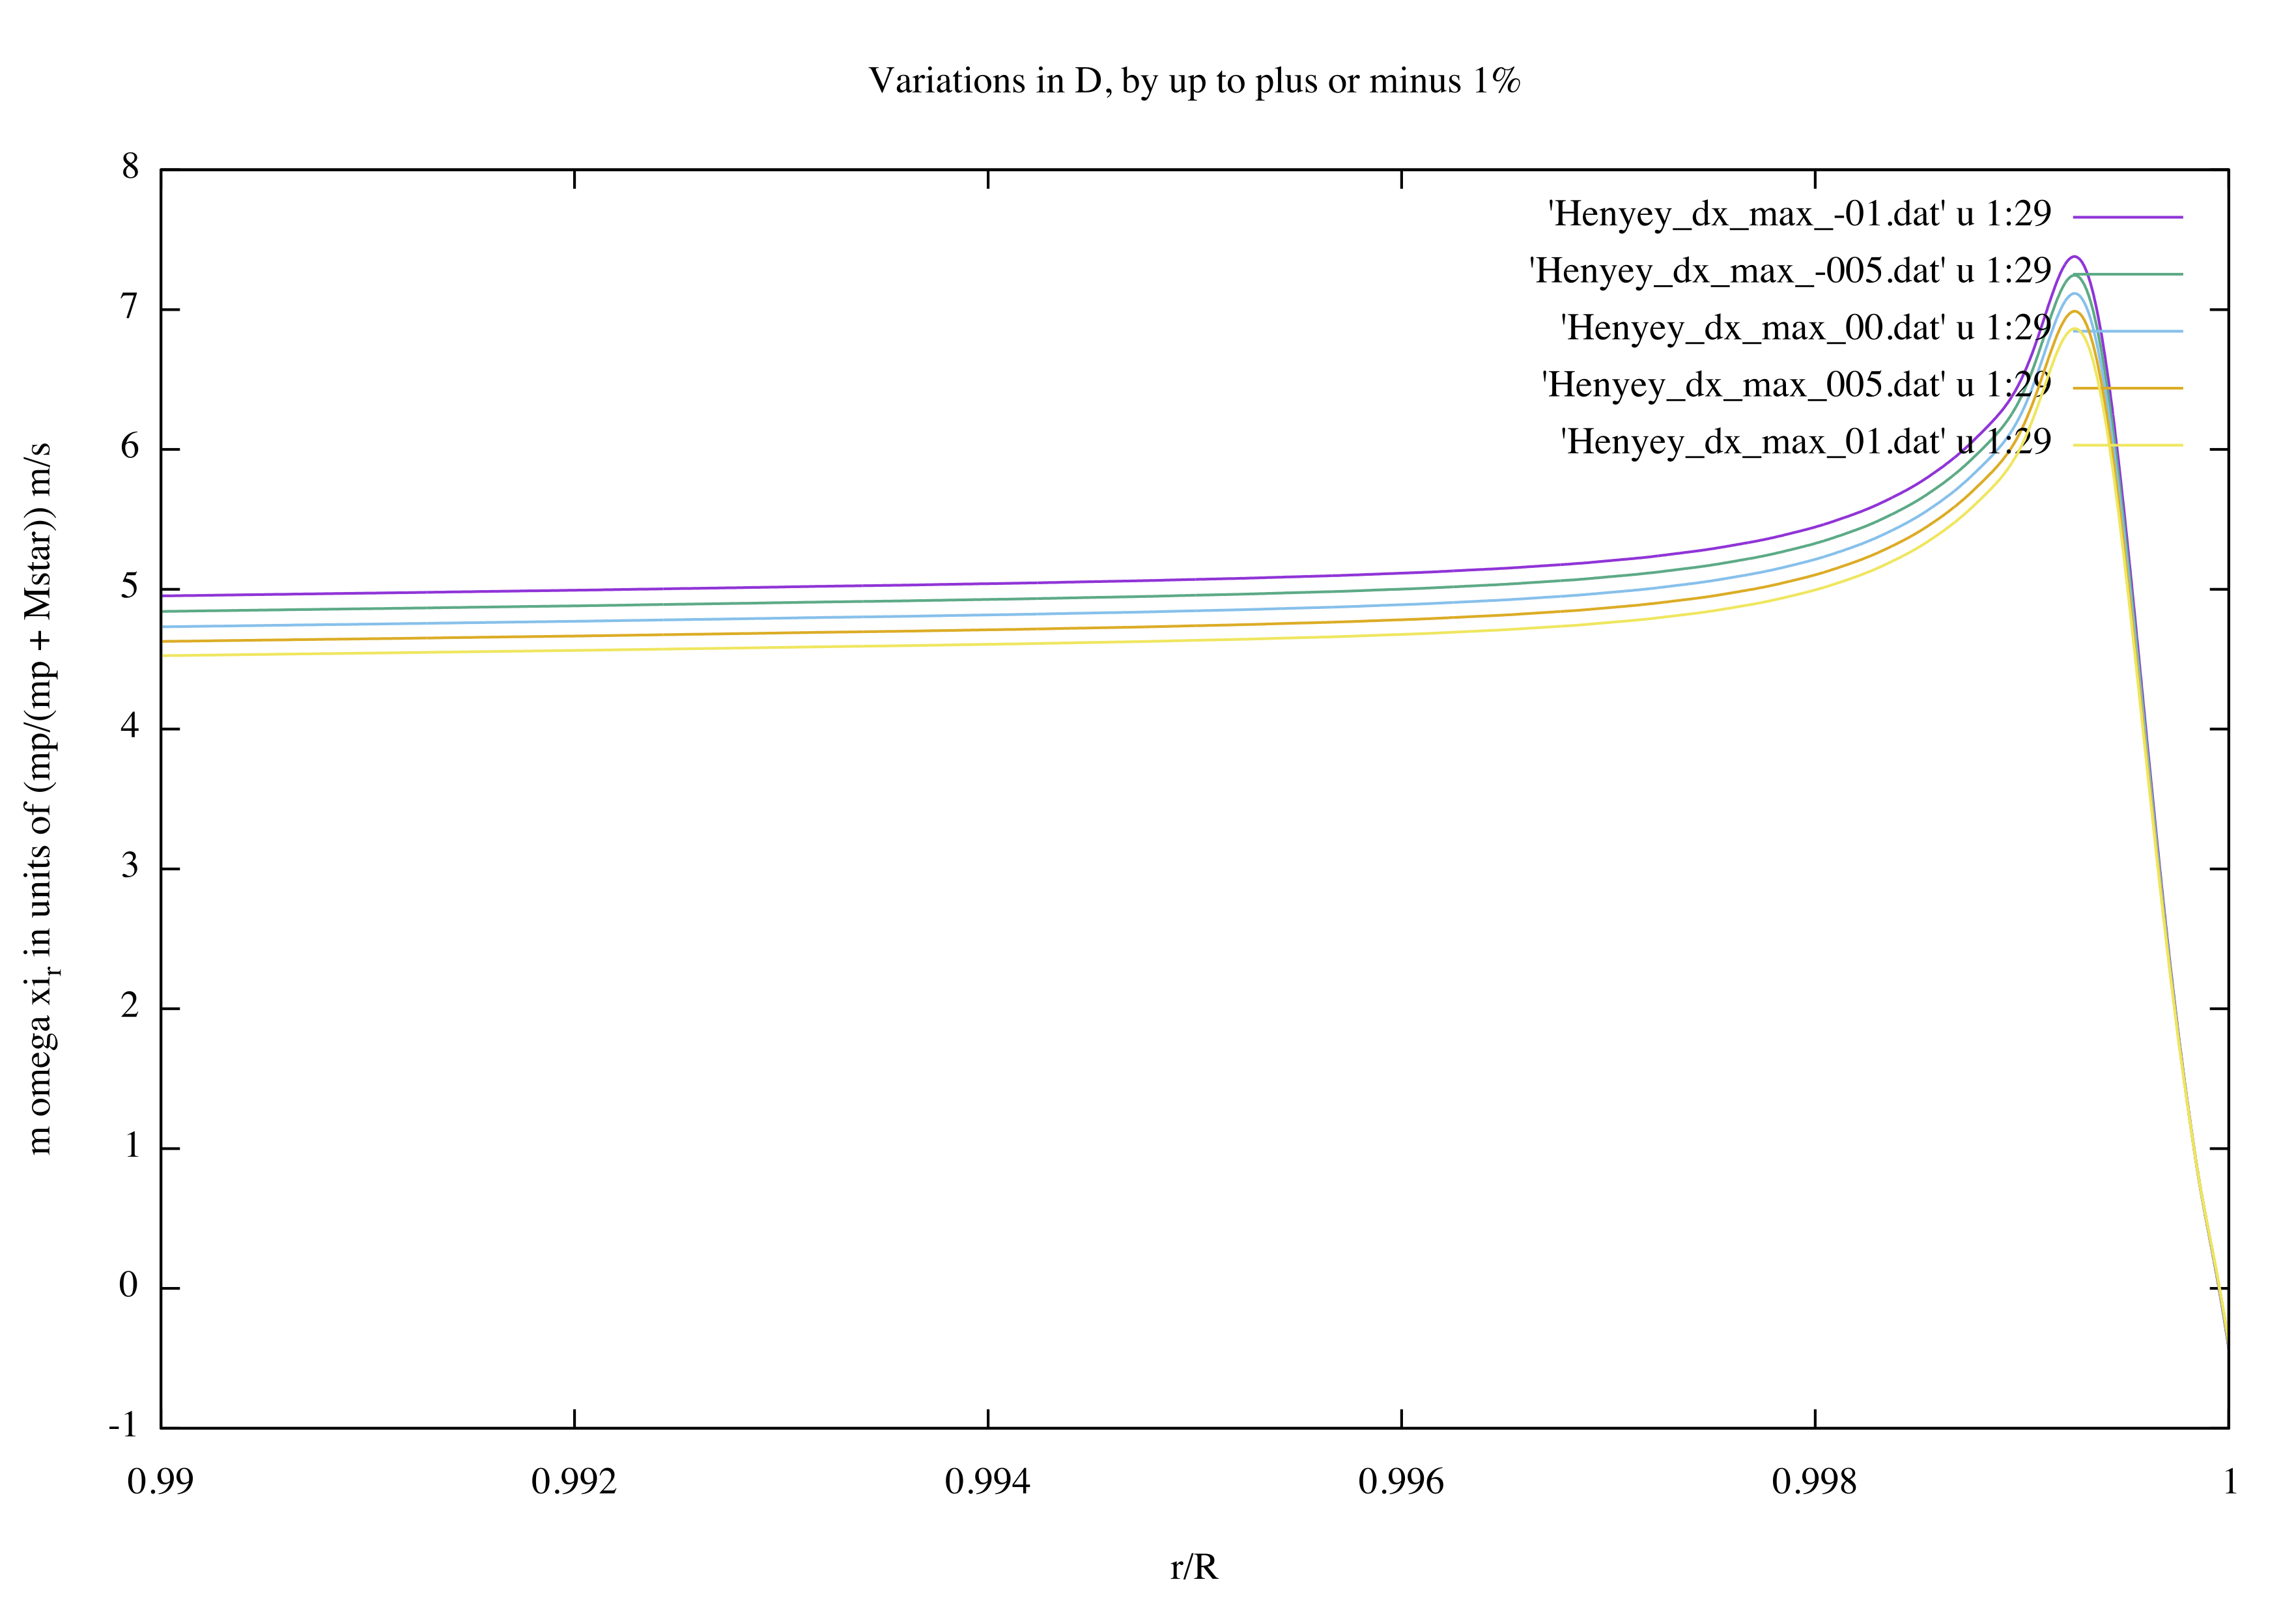
\includegraphics[width = \textwidth]{figures/xi_r_surface_Dvar.png}
\end{subfigure}

\caption{The full solution for the non-adiabatic case, showing the peak radial velocity (that is, $m \omega \xi_{r}$) in units of $\frac{m_{p}}{m_{p} + M_{*}}$ m s$^{-1}$, against the proportional radial distance from the centre.  In these figures, the semi-major axis of the planetary companion's orbit has been varied slightly, leading to a small spread in both the amplitudes and spatial frequencies of the oscillations.}
\label{fig:Dvar}
\end{center}
\end{sidewaysfigure}



The other parameter which was varied was the resolution, the outputs of which are shown in figure \ref{fig:Resvar}.  In this case, a flat limit was introduced across the whole star, rather than varying it to match the needed resolution in order to try to keep things as simple as possible.  In all cases the resolution is sufficient to resolve the oscillations, (with the lowest resolution having at least 13 points covering the shortest spatial wavelength, and the highest resolution having at least 20 points).  Similar to the case of varying $D$, varying the resolution has a significant effect on the amplitude of the oscillations towards the centre of the star, but has a totally negligible effect towards the surface.  This may be partially due to the fact that the MESA skeleton of cells is already of a higher resolution than the limits used in this case for the surface, coupled with the fact that the solution is no longer oscillatory.




\begin{sidewaysfigure}[htbp]
\begin{center}
\begin{subfigure}{0.5\textwidth}
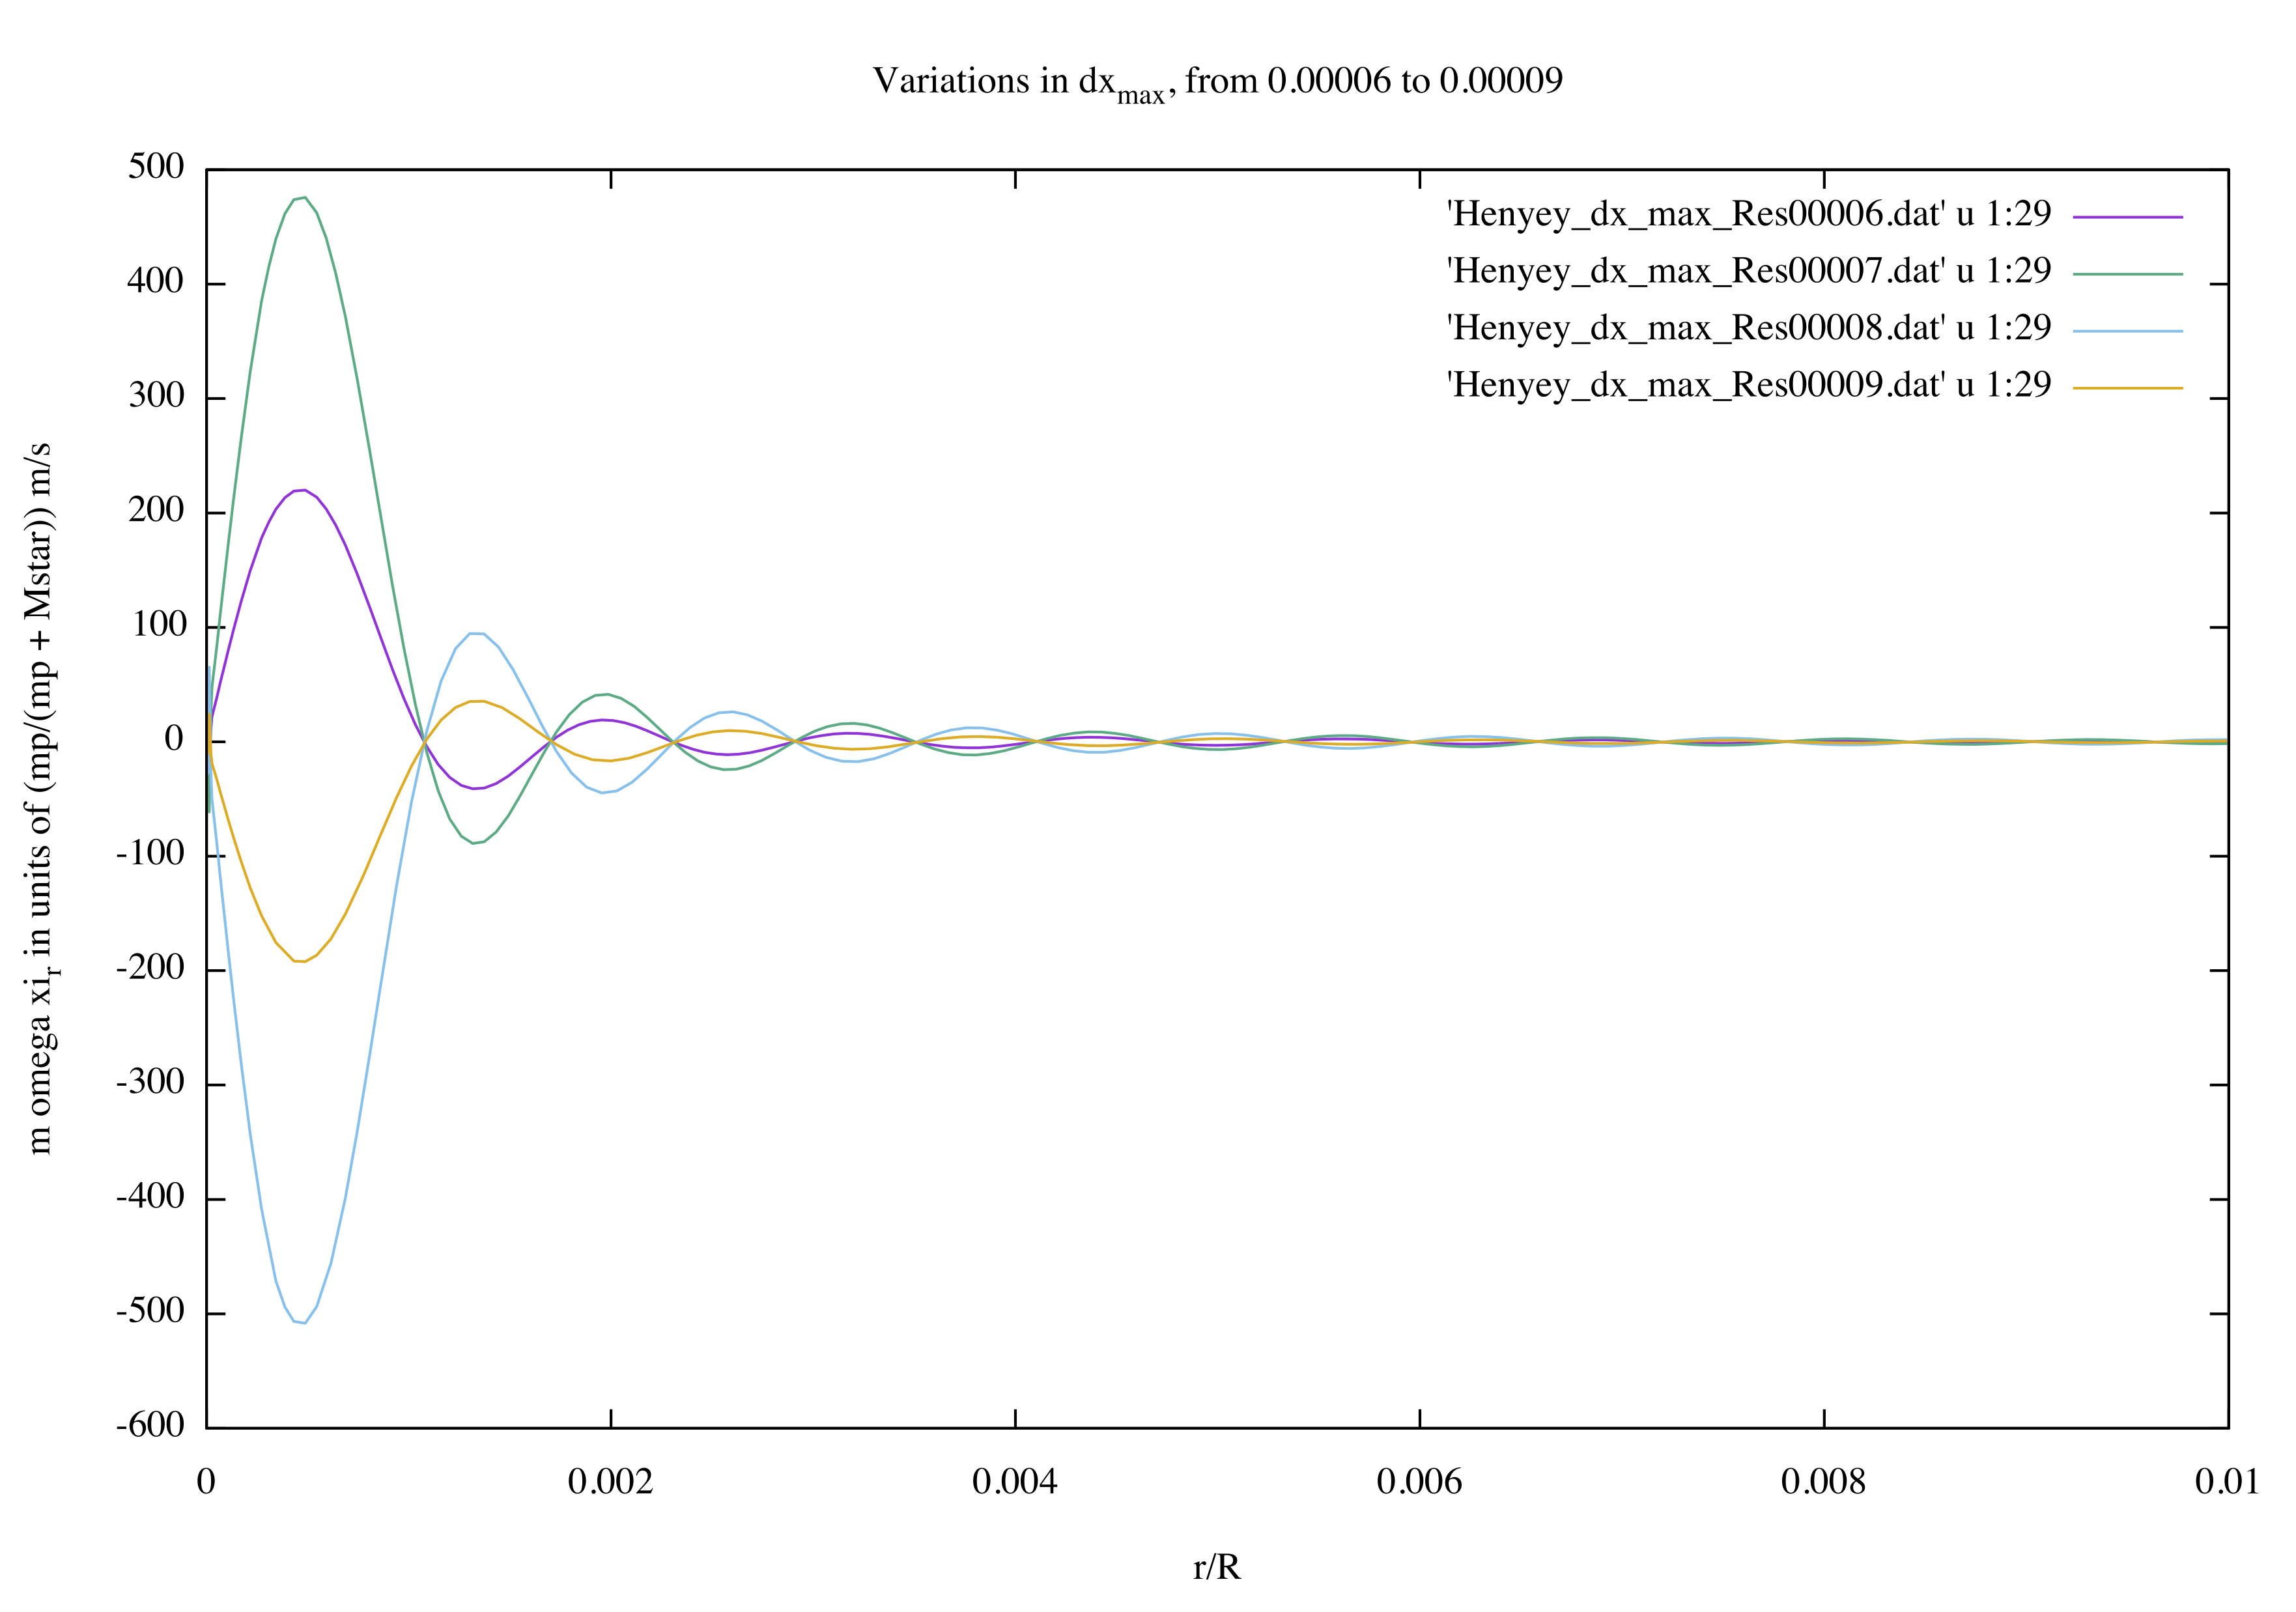
\includegraphics[width = \textwidth]{figures/xi_r_section1_Resvar.png}
\end{subfigure}
~
\begin{subfigure}{0.5\textwidth}
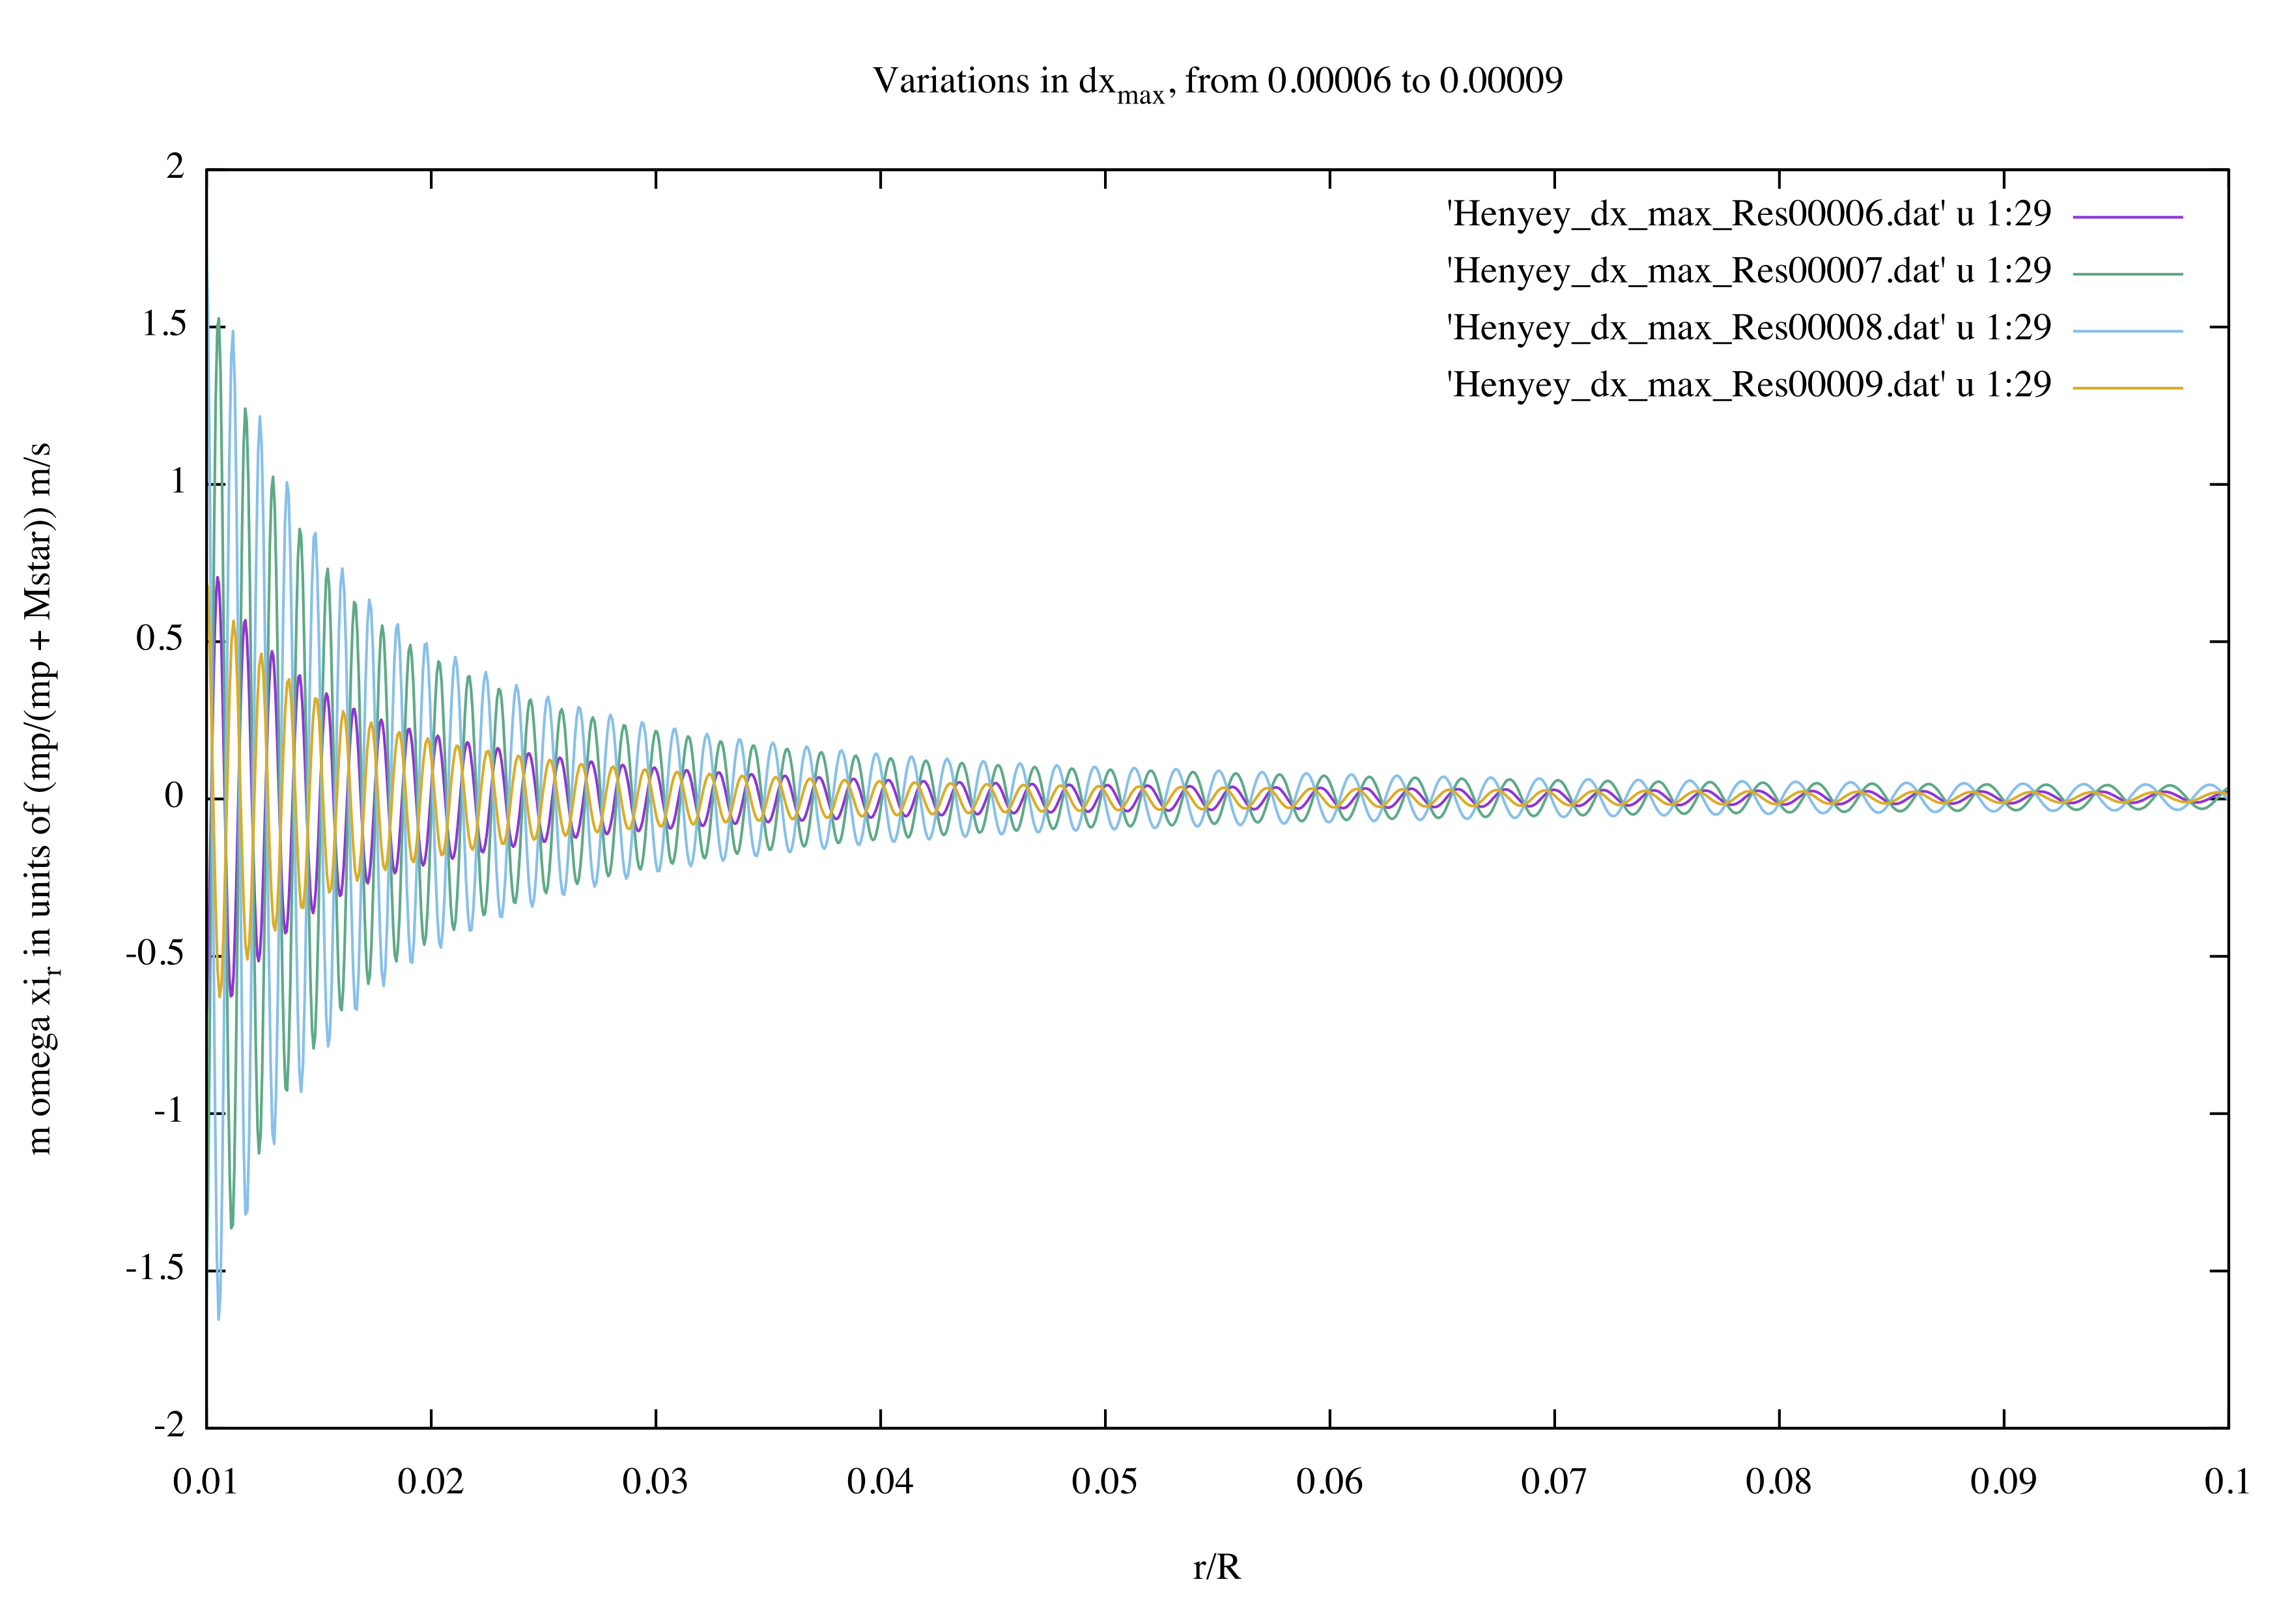
\includegraphics[width = \textwidth]{figures/xi_r_section2_Resvar.png}
\end{subfigure}

\begin{subfigure}{0.5\textwidth}
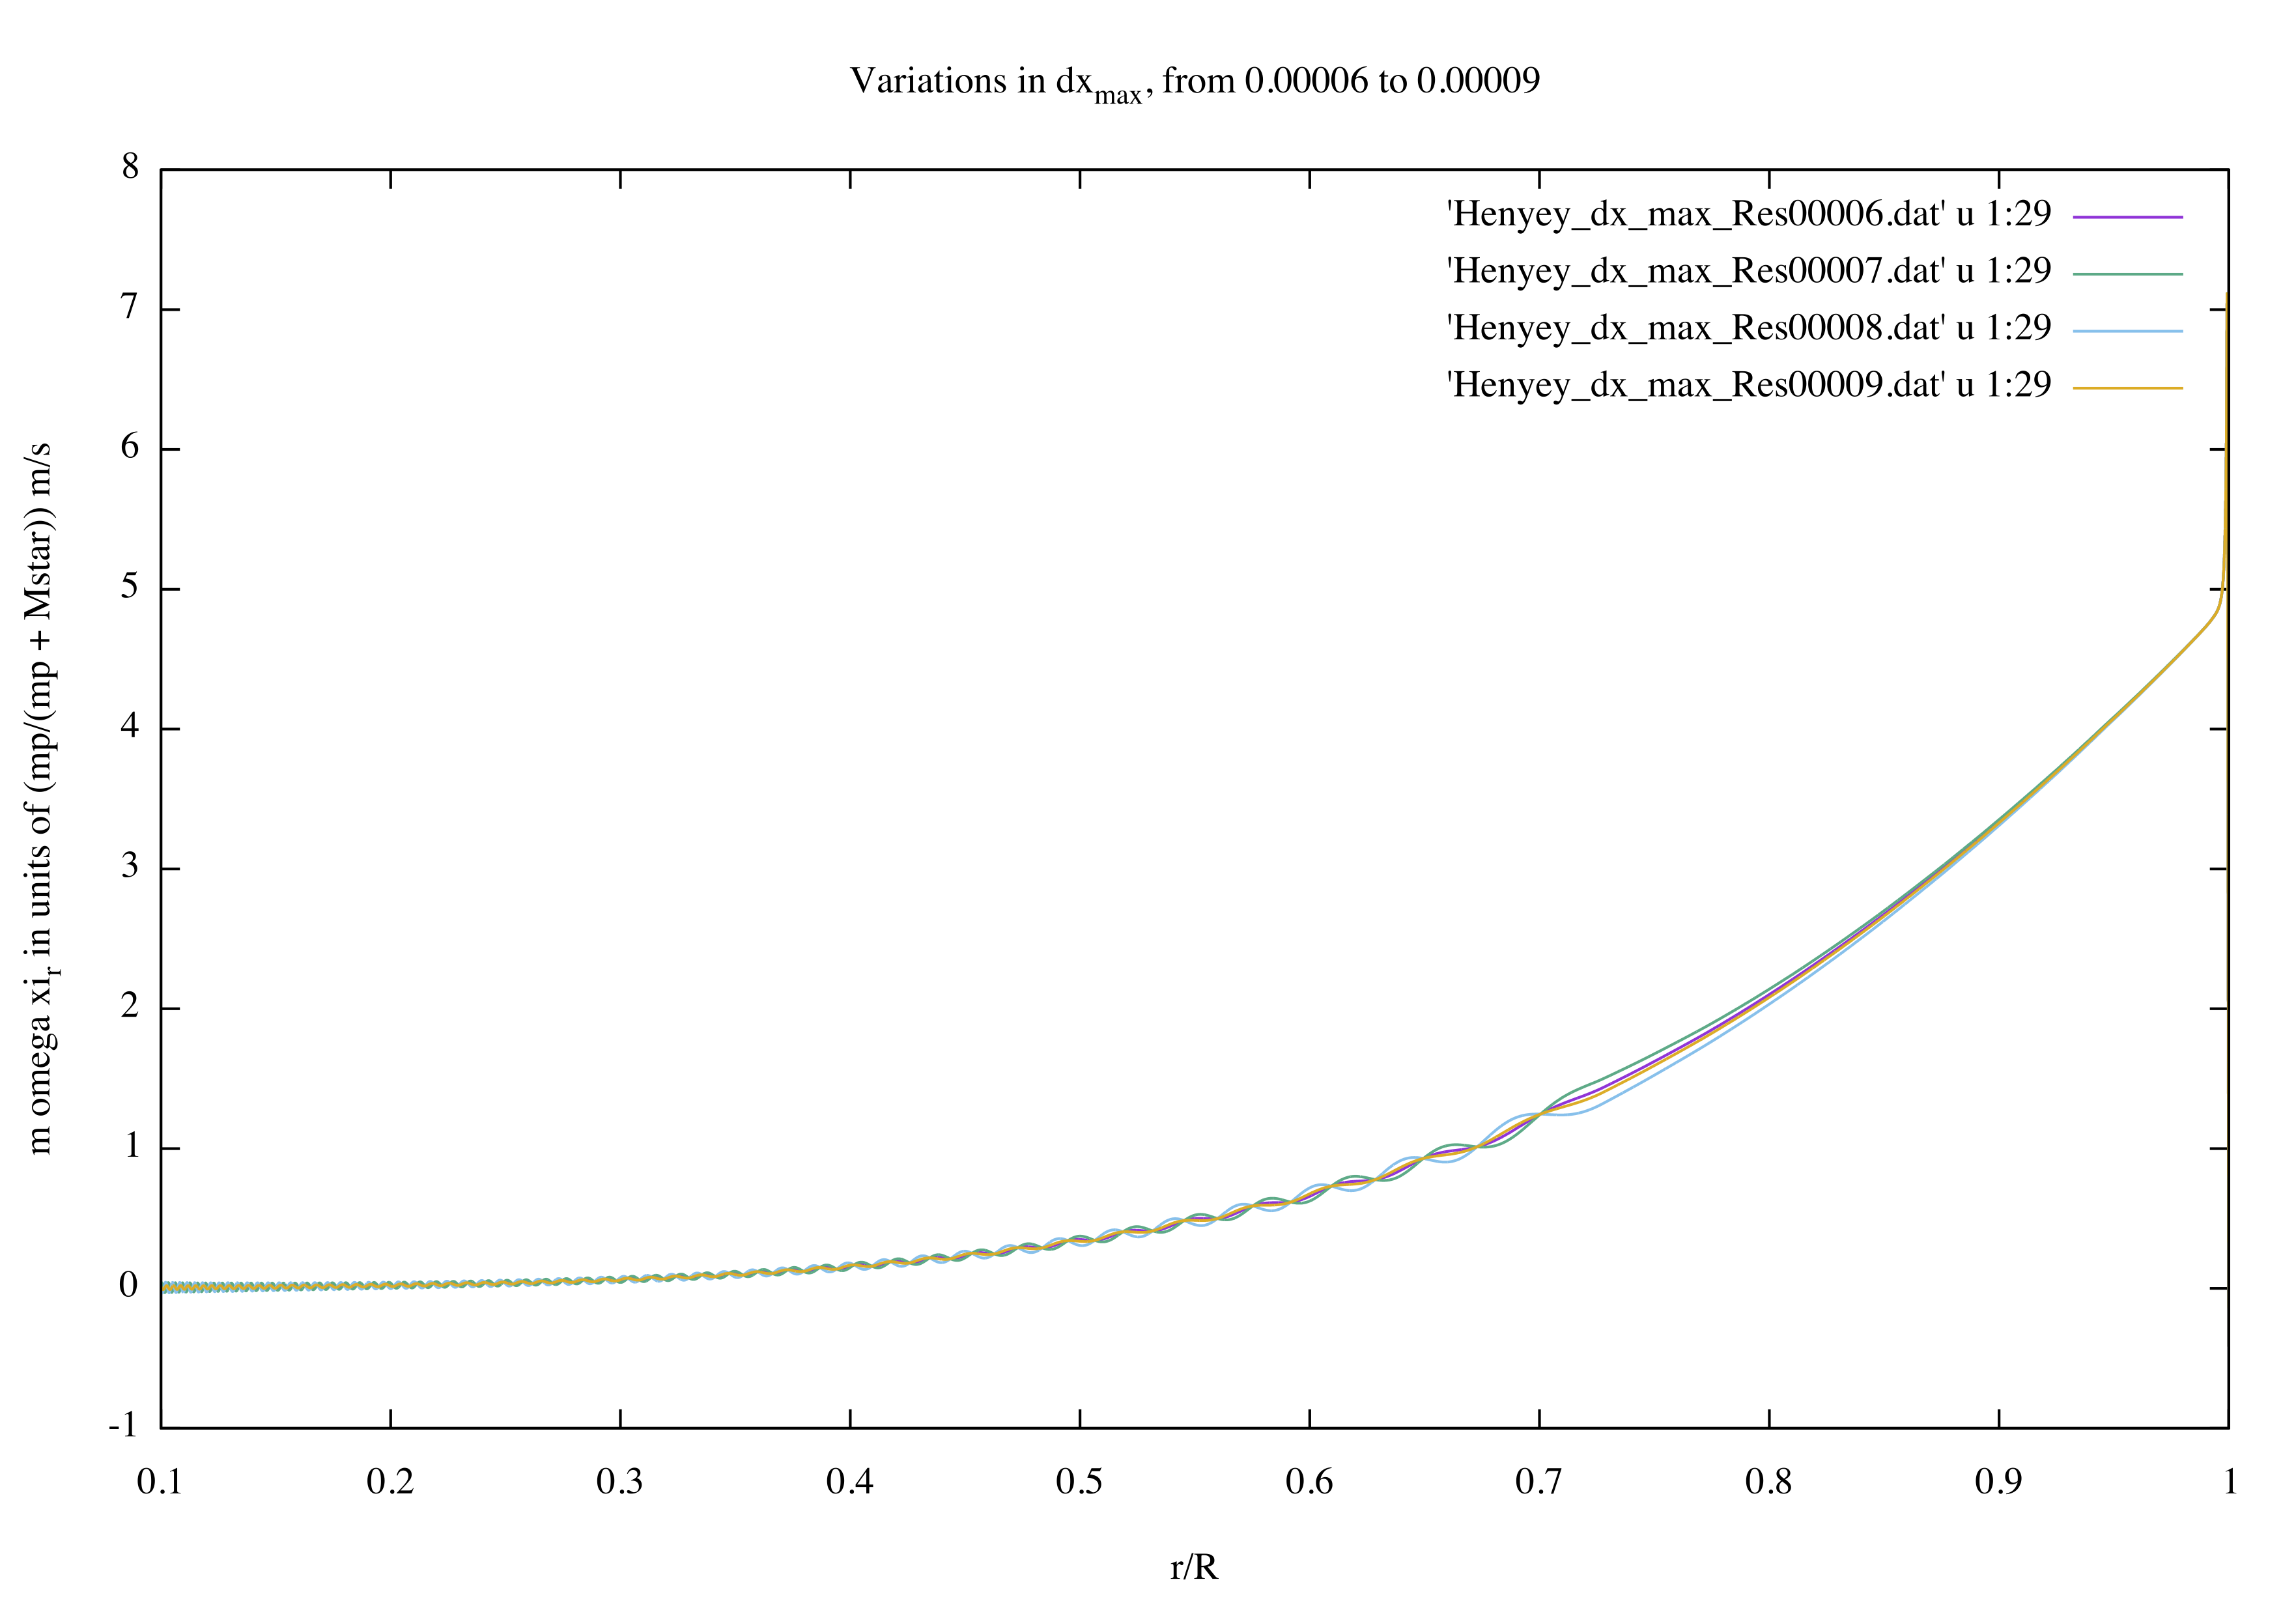
\includegraphics[width = \textwidth]{figures/xi_r_section3_Resvar.png}
\end{subfigure}
~
\begin{subfigure}{0.5\textwidth}
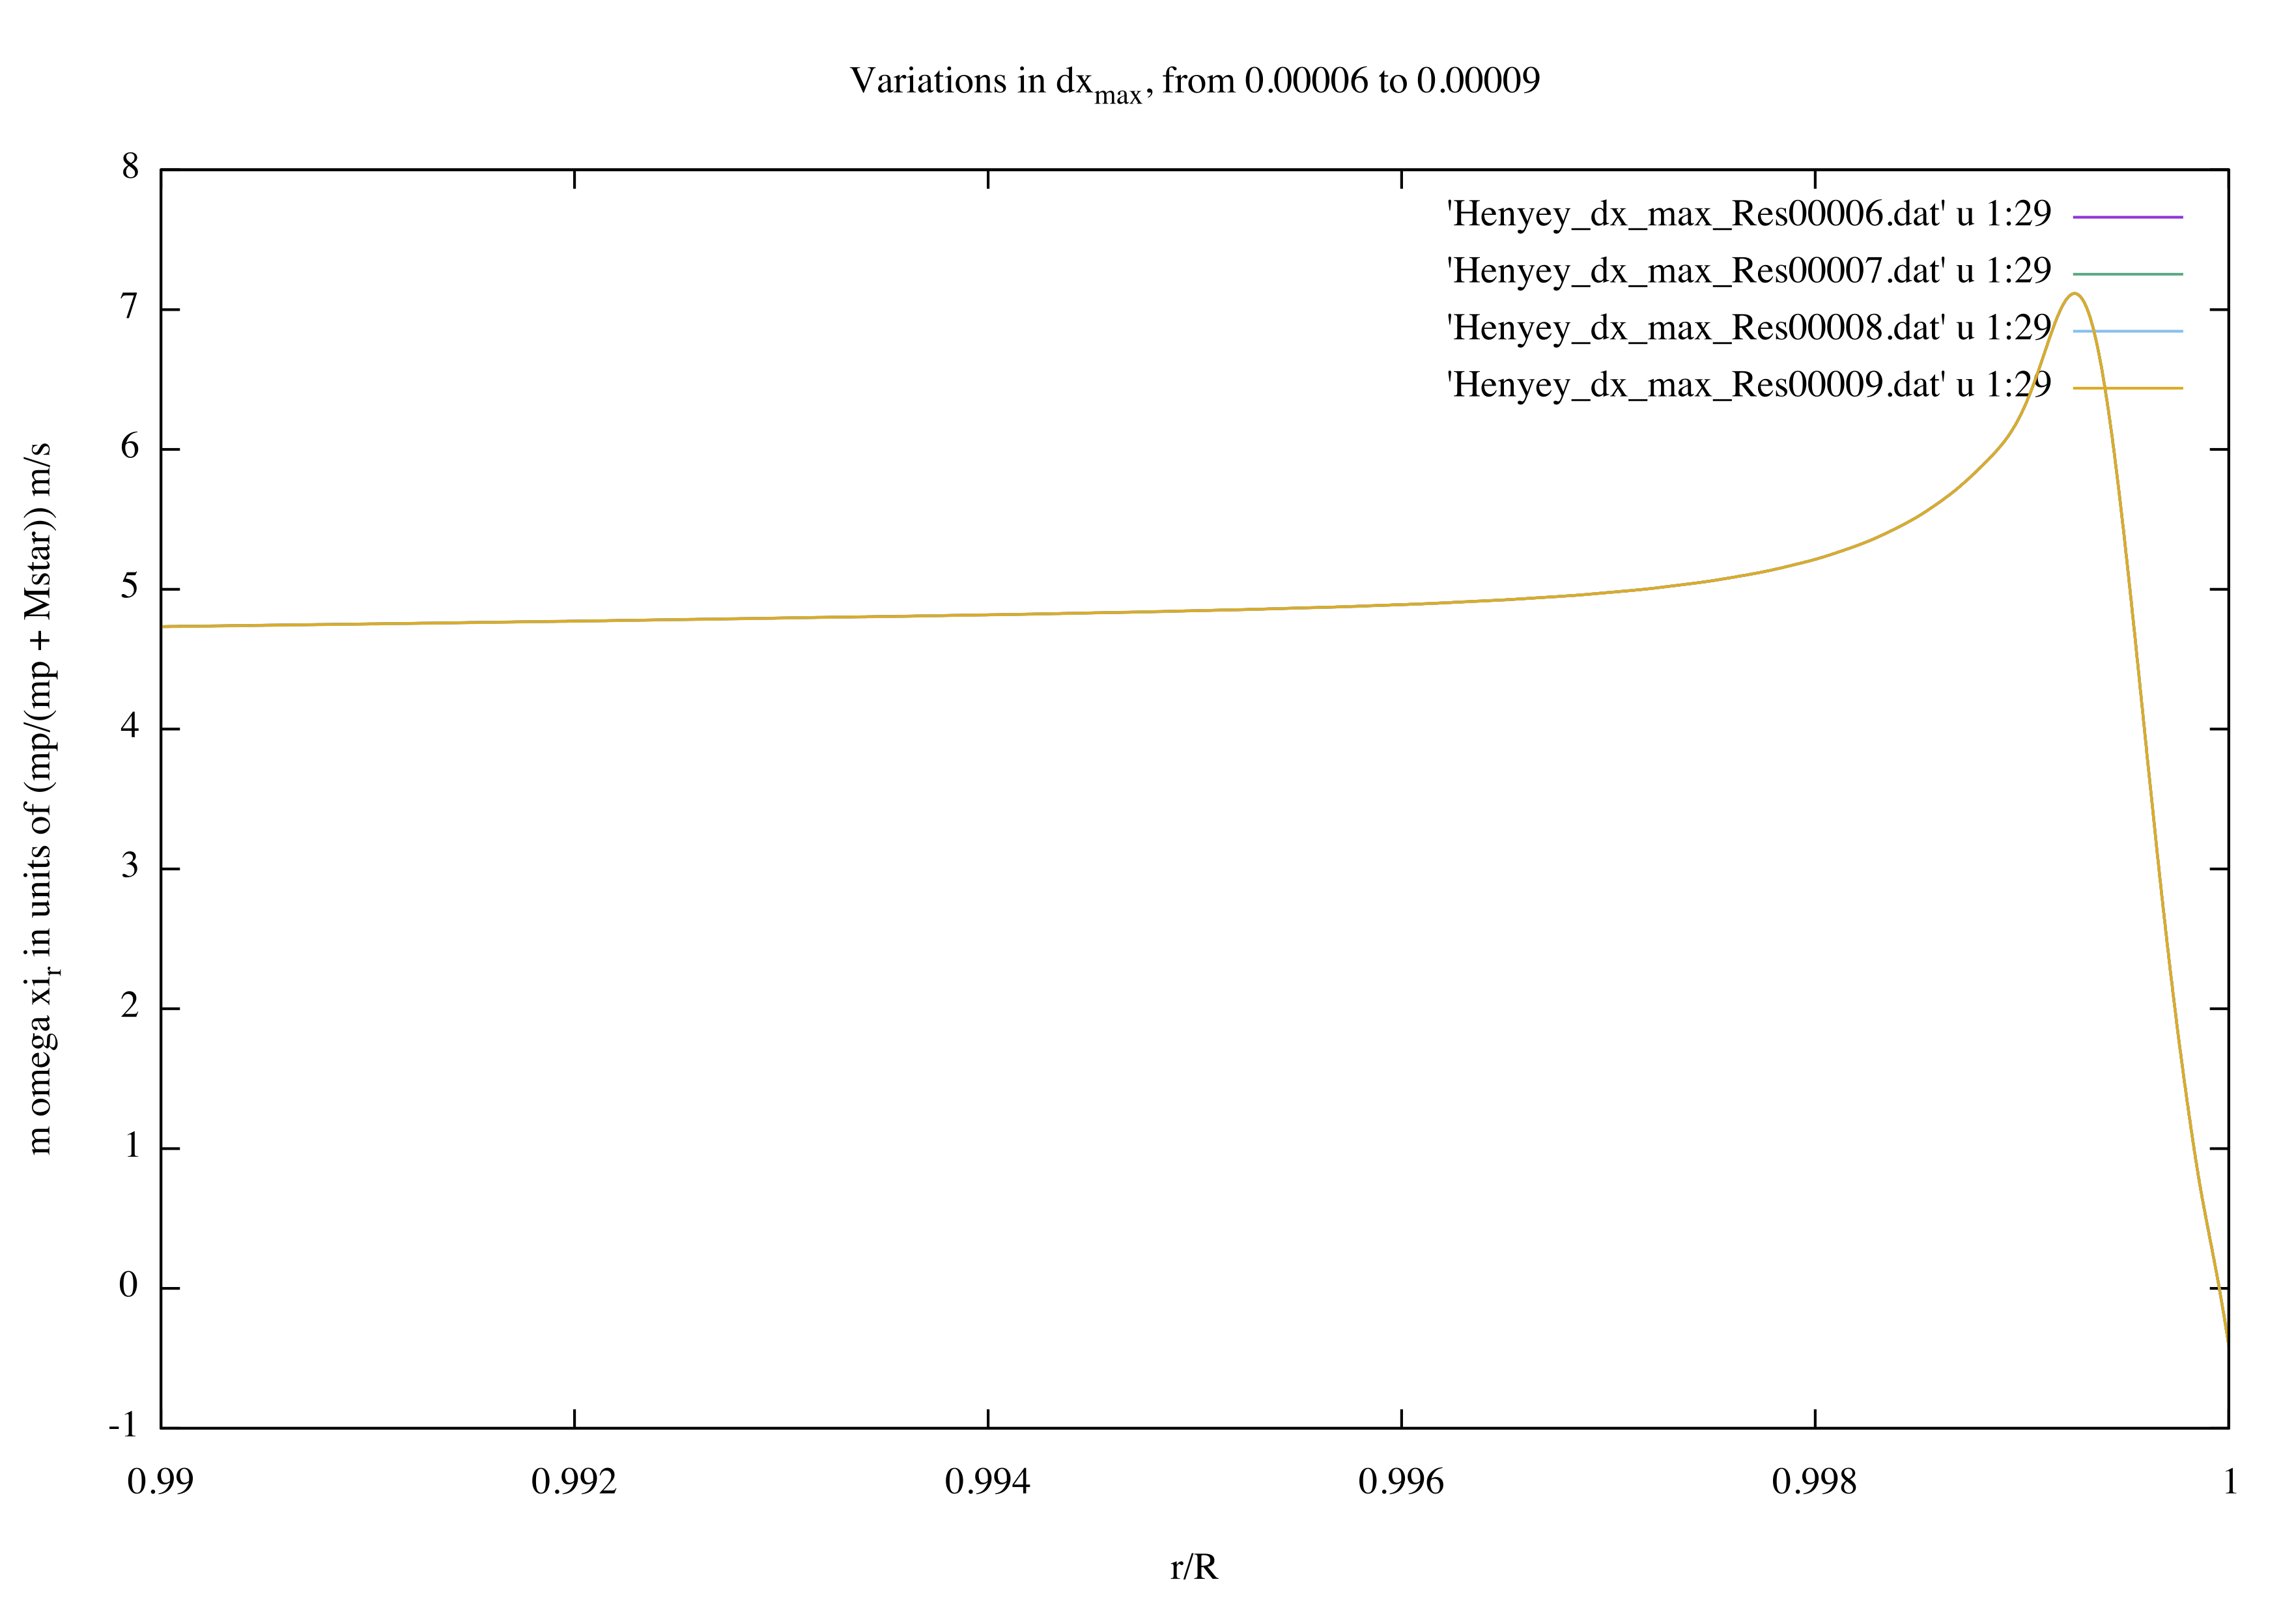
\includegraphics[width = \textwidth]{figures/xi_r_surface_Resvar.png}
\end{subfigure}

\caption{The full solution for the non-adiabatic case, showing the peak radial velocity (that is, $m \omega \xi_{r}$) in units of $\frac{m_{p}}{m_{p} + M_{*}}$ m s$^{-1}$, against the proportional radial distance from the centre.  In these figures the maximum cell size, and therefore the resolution limit of the grid, has been varied slightly, leading to a spread in the amplitudes of the oscillations.  The maximum cell size, as a proportion of the stellar radius, is plotted at $6 \times 10^{-5}$ (purple line), $7 \times 10^{-5}$ (green line), $8 \times 10^{-5}$ (blue line), and $9 \times 10^{-5}$ (orange line).}
\label{fig:Resvar}
\end{center}
\end{sidewaysfigure}





Where there is variation in the amplitude, the spatial wavelengths are still unaffected, and the overall patterns of behaviour are very similar for all the resolutions.  This is encouraging, as it shows that, although resolution may limit the extent to which we can extract precise quantitative data from the central regions, the nature and behaviour of the waves, both oscillatory and evanescent, seems to be unaffected.  As such, whilst it is clear that a higher resolution is desirable, it does not limit the usefulness of the output any more than the physical limits in the precision of the parameters of the system do (as shown in figure \ref{fig:Dvar}).


A final point to consider is the validity of the assumptions made in the derivation of the equations (listed in section \ref{Intro:StellarOsc}), to check that the solution is consistent with them.  This essentially boils down to ensuring that the perturbations are small at all points throughout the star, which can be assessed by checking the output throughout the entirety of the star.  Where this assumption is likely to break depends on the variables: $\xi_{r}$ and $F_{r}'$ are most likely to be comparable to the local equilibrium values ($r$ and $F_{r}$) towards to core of the star; $p'$ and $T'$ are most likely to comparable towards the surface.  In the case tested here, other than a few points in the value of $F_{r}'$ at the very core, all points are $\ll 1$.  These very core points are not thought to be much of an issue, as they seem to just be an edge effect, which has no apparent impact on the rest of the solution, and quickly decays away.



Overall, the code is well tested, and reproduces previous results well.  It is easy to apply to any model created in MESA, and the stability of the solution can be simply tested by investigating the effect of small variations in parameters, enabling the expected errors to be very simply and effectively assessed, and the code can be adapted and continually tested to ensure that the equations remain valid in all cases.






\section{Conclusion} \label{Conc}


Overall, the project has started well, with the production of an effective, quick and adaptable code which can be used to accurately solve the stellar oscillation equations.  The code's limitations have been explored, including both errors due to limited physical knowledge and limitations inherent in the numerical calculation.

There are many observed systems to which this code could be applied, as well as multiple different avenues of further research, which will be discussed in the section \ref{Future}.  The outputs of this code are useful, and will be able to be compared to observations soon, as they can be translated into both photometric and spectroscopic effects, which will enable the accuracy of stellar models to be tested, and will also lead to improved methods for detecting subsequent planets in systems with an observed Hot Jupiter.

Furthermore, the code is adaptable, in that the source of the perturbation could be changed in order to model another cause of oscillations, and that the code can be expanded to address different modes of oscillation, stellar rotation, or eccentric planetary orbits.







\section{Further Work}   \label{Future}

The immediate next step is to convert the calculated properties of the oscillations into relevant observables -- both in terms of the spectroscopic and photometric effects.  Spectroscopically, the Doppler shift from the motion of the surface at each point along the line of sight of the observer would be calculated to model the total lineshape as a result of the oscillations.  Photometrically, the change in shape, and the perturbed flux would contribute to a change in the total brightness of the object.  Both calculations would also need to account for the inclination of the orbit relative to the observer.  This combination of the current work with these extensions, applied to a number of known systems (such as Pegasi 51b, HD 189733 b and HD 209458 b) would form a paper over the next six months.

Work beyond that would depend on the results produced in the next few months.  One major avenue for investigation would be the use of tidally induced oscillations in exoplanet detection in the case of inclined planets -- such that transits are not observable, and RV measurements alone may be inconclusive.  Another would be the behaviour of advanced stars under tidal forcing, and the implications for multiple planet detection around such stars, which would include the study of both Red Giants and White Dwarfs.  The code could also be applied to the case of stellar binaries, and the oscillations induced on both stars would be modelled.  

The code as a whole could be broadened in its scope, by extending the realm over which the code is applicable: allowing for stellar rotation, eccentric orbits, and higher order perturbations.  This would apply to all of the above in terms of extending the relevancy and scope of research, and could enable better characterisation of systems, by being able to constrain the rotation of stars by comparing the predicted and observed results.  There are also published results regarding the modelled dynamical tides in stars as a result of rotation and eccentric orbits \cite{Burkart2012} against which the code could be once more tested and calibrated.

Overall, there are several possible, realistic and valuable avenues down which this research could continue, which could make predictions which could be used to potentially direct the use of observing time, particularly in the hunt for exoplanets, and even to test the accuracy of stellar modelling across a range of scenarios.









\section{Acknowledgements}  \label{Acknowledgements}

I would like to acknowledge the input of my supervisor, Caroline Terquem,  and of John Papaloizou, in the form of guidance and discussion throughout this project.

I would like to acknowledge MESA, \cite{Paxton2011}. http://mesa.sourceforge.net/index.html

This research has made use of the NASA Exoplanet Archive, which is operated by the California Institute of Technology, under contract with the National Aeronautics and Space Administration under the Exoplanet Exploration Program.





\bibliographystyle{plain}
\bibliography{library}









\newpage

\appendix

\section{Stellar Oscillation Equations} \label{ap:Osc}



This is a record of the basic equations from which the non-adiabatic non-radial oscillation
equations are derived. The process is fairly simple -- the equations are linearised using small
perturbations to the spherically symmetric, time-independent equilibrium state. The Cowling
approximation is used, which says that the self-gravity of the star is negligibly affected by the
oscillations, so the perturbation to the gravitational potential in this case comes purely from the
orbiting planet. EM body forces, viscous forces and energy source terms (such as nuclear fusion and
heat from viscous dissipation) are all neglected.


\subsection{Basic Equations}


\subsubsection{Assumptions}

The equilibrium case is taken to be time-independent (or at least changing on a time-scale much 
smaller than the time-scale of the oscillations), spherically symmetric (therefore equilibrium 
quantities are functions only of the radius, r), and static (such that the fluid velocity of 
equilibrium, $\vec{u}_{0} = 0$).

In this analysis, we will also use the Cowling approximation, which states that the perturbation
to the self-gravity potential is negligible.  Therefore the perturbation to $\Phi$ is given by 
the potential due to the perturbing body, $\Phi_{P}$.



\subsubsection{Linearising}

To study effects of infinitesimal perturbations to the system, the variables are expanded into
their equilibrium and perturbed components, such as $q = q_{0} + q'$, for some variable, $q$.
The equilibrium quantities themselves satisfy the fluid equations, so cancel out.  Terms which are
second order in perturbed quantities are taken to be negligible, because the perturbation is
taken to be very small. This leaves only terms which are linear in perturbed quantities.

Looking at the perturbed velocity in particular, and recalling that the equilibrium state is taken
to be static, we see that $\vec{u} = 0 + \vec{u}'$.  We can re-express this in terms of $\vec{\xi}$,
 the displacement from equilibrium ($\vec{\xi} = \vec{r} - \vec{r}_{0}$).  Relating the Lagrangian and 
Eulerian descriptions of the perturbed velocity gives:

\begin{equation}
\delta \vec{u} = \vec{u}' + (\vec{\xi} \cdot \vec{\nabla}) \vec{u}_{0} \longrightarrow \delta \vec{u} = \vec{u}'
\end{equation}
\\
which shows that the perturbed velocity is the same in both the Eulerian and Lagrangian descriptions.

We can then use this to relate the displacement to the perturbed velocity, as

\begin{equation}
\delta \vec{u} = \vec{u}(\vec{r}_{0} + \vec{\xi}) - \vec{u}(\vec{r}_{0}) = \frac{d\vec{r}}{dt} - \frac{d\vec{r}_{0}}{dt}
= \frac{d}{dt} \left( \vec{r} - \vec{r}_{0} \right) = \frac{d}{dt} \vec{\xi}
\end{equation}
\\
and as $\delta\vec{u} = \vec{u}'$, we can also say that $\vec{u} = \frac{\partial \vec{\xi}}{\partial t}$.






\subsubsection{Continuity equation}

The continuity equation is a result from the conservation of mass, and can be expressed as

\begin{equation} \frac{\partial \, \rho}{\partial \, t} + \vec{\nabla} \cdot ( \rho \, \vec{u} )
\end{equation}
\\
where $\rho$ is the density.  This is linearised to

\begin{equation}
\frac{\partial}{\partial t} \left( \rho' + \vec{\nabla} \cdot \left( \rho_{0} \vec{\xi} \right) \right) = 0
\end{equation}
\\
using the fact that the equilibrium quantities are time-independent to bring the partial time
derivative outside the brackets.



\subsubsection{Momentum equation}

This equation arises from examining the forces acting on a fluid element, given as

\begin{equation} \rho \left( \frac{\partial}{\partial \, t} +  \vec{u} \cdot \vec{\nabla} \right)
\vec{u} = \rho \vec{f} - \vec{\nabla} p - \rho \vec{\nabla} \Phi + \vec{\nabla} \cdot \hat{\Pi}
\end{equation}
\\
where $p$ is the pressure, , $\Phi$ is the gravitational potential, $\vec{f}$ is
the EM and external forces per unit volume, and $\hat{\Pi}$ is the viscous stress tensor. In this
case, $\vec{f}$ and $\hat{\Pi}$ may be neglected, as the fluid is almost an ideal gas, is charge
neutral, and the only external influence is gravitational, which is taken into account by $\Phi$.

Linearising this, we use the Cowling approximation to use the substitution $\Phi = \Phi_{0} + \Phi_{P}$.
This gives

\begin{equation}
\rho_{0} \frac{\partial^{2} \vec{\xi}}{\partial t^{2}} = - \vec{\nabla} p' - \rho_{0} \vec{\nabla} \Phi_{P}
- \rho' \vec{\nabla} \Phi_{0}.
\end{equation}



\subsubsection{Energy equation}

This equation arises from considering the release and flux of energy and can be expressed as

\begin{equation}
\rho T \left( \frac{\partial}{\partial t} + \vec{u} \cdot \vec{\nabla} \right) s =
\rho \left( \epsilon_{N} + \epsilon_{\nu} \right) - \vec{\nabla} \cdot \vec{F}
\end{equation}
\\
where $s$ is the specific entropy, $\epsilon_{N}$ is the specific nuclear energy generation rate,
$\epsilon_{\nu}$ is the specific rate of release of heat due to viscosity, and $\vec{F}$ is the radiative flux.

In linearising, we neglect both $\epsilon_{N}$ and $\epsilon_{\nu}$, as we expect the nuclear energy
generation rate to be insensitive to the small perturbations (and nuclear energy generation will only
occur in a small region at the core, where oscillations are expected to be smallest) and we are
neglecting viscosity still.

\begin{equation}
\rho_{0} T_{0} \frac{\partial}{\partial t} \left( s' + \vec{\xi} \cdot \vec{\nabla} s_{0} \right)
= s - \vec{\nabla} \cdot \vec{F}.
\end{equation}
\\

\subsubsection{Associated equations}

These equations are necessary to relate variables to each other, particularly in terms of gradients of
equilibrium quantities.

First, we have the express the radiative flux using the radiative diffusion equation as

\begin{equation}
\vec{F} = - K \vec{\nabla} T
\end{equation}
\\
where $K = \frac{4 a c_{*}}{3 \kappa \rho} T^{3}$, where $a = \frac{4 \sigma}{c_{*}} = 7.5657 \times 10^{-15}$ 
erg cm$^{-3}$ K$^{-4}$ is the radiation density constant ($\sigma$ is the Stefan-Boltzmann constant),
$c_{*}$ is the speed of light (the subscript-asterisk is to differentiate it from the sound speed) 
and $\kappa$ is the opacity.

Linearising will give us

\begin{equation}
\vec{F}' = - K' \vec{\nabla} T_{0} - K_{0} \vec{\nabla} T'
\end{equation}
\\
and

\begin{equation}
\frac{K'}{K_{0}} = 3 \frac{T'}{T_{0}} - \frac{\kappa'}{\kappa_{0}} - \frac{\rho'}{\rho_{0}}.
\end{equation}
\\

We must also find a relation for the change in opacity, the change in density, and the change in specific entropy,
in terms of the variables of state which we are most interested in.  For the most part, this
means expressing total derivatives in terms of $p$ and $T$, but not always -- this is largely
dictated by the derivatives which are available through MESAstar.

For the opacity, we express it as $\kappa = \kappa \left( \ln (\rho) , \ln(T) \right)$, which gives us

\begin{equation}
d\kappa = \left( \frac{\partial \kappa}{\partial \ln \rho} \right)_{T} d(\ln \rho) + \left( \frac{\partial \kappa}{\partial \ln T} \right)_{\rho} d(\ln T)
\end{equation}
\\
which is linearised to give

\begin{equation}
\kappa' = \left( \frac{\partial \kappa}{\partial \ln \rho} \right)_{T} \frac{\rho'}{\rho_{0}} + \left( \frac{\partial \kappa}{\partial \ln T} \right)_{\rho} \frac{T'}{T_{0}}
\end{equation}
\\
which is left in this form, as the partial derivatives in this form are available as an output from MESAstar.



\subsubsection{Thermodynamic equations}

Two more equations are required to relate a couple of specific quantities to the variables of interest.
Both the specific entropy and the density are taken to be functions of $T$ and $p$, and their total derivatives
are expanded accordingly.  This gives rise to:

\begin{equation}
ds = \left( \frac{\partial s}{\partial p} \right)_{T} dp +\left( \frac{\partial s}{\partial T} \right)_{p} dT
\end{equation} 
\\
and we substitute in $c_{p} = T \left( \frac{\partial s}{\partial T} \right)_{p}$ and 
$\nabla_{ad} = \left( \frac{\partial \ln T}{\partial \ln p} \right)_{s} = \frac{p_{0}}{T_{0}} \left( \frac{\partial T}{\partial p} \right)_{s}$ used in conjunction with
the triple product rule to give

\begin{equation}
s' = - \left( \frac{\partial s}{\partial T} \right)_{p} \left( \frac{\partial T}{\partial p} \right)_{s} p' +\left( \frac{\partial s}{\partial T} \right)_{p} T'
= - \frac{c_{p}}{T_{0}} \frac{T_{0}}{p_{0}} \nabla_{ad} p' + \frac{c_{p}}{T_{0}} T'
\end{equation} 
\\
which then leaves us with

\begin{equation}
s' = c_{p} \left( \frac{T'}{T_{0}} - \nabla_{ad} \frac{p'}{p_{0}} \right).
\end{equation} 
\\
Similarly, for the density, we introduce $\chi_{\rho} \equiv \left( \frac{\partial \ln p}{\partial \ln \rho} \right)_{T}$
 and $\chi_{T} \equiv \left( \frac{\partial \ln p}{\partial \ln T} \right)_{\rho}$, and once again use the 
 triple product rule to give
 
\begin{equation}
d \ln \rho = \left( \frac{\partial \ln \rho}{\partial \ln p} \right)_{T} d \ln p + \left( \frac{\partial \ln \rho}{\partial \ln T} \right)_{p} d \ln T
= \left( \frac{\partial \ln \rho}{\partial \ln p} \right)_{T} \frac{p'}{p_{0}} - \left( \frac{\partial \ln \rho}{\partial \ln p} \right)_{T} \left( \frac{\partial \ln \rho}{\partial \ln T} \right)_{\rho} \frac{T'}{T_{0}}
\end{equation} 
\\
which can be finally expressed as

\begin{equation}
\frac{\rho'}{\rho_{0}}= \frac{1}{\chi_{\rho}} \left( \frac{p'}{p_{0}} - \chi_{T} \frac{T'}{T_{0}} \right)
\end{equation}
\\
which completes the set of equations which we need.






\subsubsection{List of linearised equations}

We are then left with the following linearised equations, which will then need to be cut down such that solving
the system becomes a practical task.


\begin{equation} \label{eq:cont_lin}
\frac{\partial}{\partial t} \left( \rho' + \vec{\nabla} \cdot \left( \rho_{0} \vec{\xi} \right) \right) = 0
\end{equation}


\begin{equation} \label{eq:mom_lin}
\rho_{0} \frac{\partial^{2} \vec{\xi}}{\partial t^{2}} = - \vec{\nabla} p' - \rho_{0} \vec{\nabla} \Phi_{P}
- \rho' \vec{\nabla} \Phi_{0}
\end{equation}

\begin{equation} \label{eq:E_lin}
\rho_{0} T_{0} \frac{\partial}{\partial t} \left( s' + \vec{\xi} \cdot \vec{\nabla} s_{0} \right)
= - \vec{\nabla} \cdot \vec{F}'
\end{equation}


\begin{equation} \label{eq:F_lin}
\vec{F}' = - K' \vec{\nabla} T_{0} - K_{0} \vec{\nabla} T'
\end{equation}



\begin{equation} \label{eq:K_lin}
\frac{K'}{K_{0}} = 3 \frac{T'}{T_{0}} - \frac{\kappa'}{\kappa_{0}} - \frac{\rho'}{\rho_{0}}.
\end{equation}



\begin{equation} \label{eq:kap_lin}
\kappa' = \left( \frac{\partial \kappa}{\partial \ln \rho} \right)_{T} \frac{\rho'}{\rho_{0}} + \left( \frac{\partial \kappa}{\partial \ln T} \right)_{\rho} \frac{T'}{T_{0}}
\end{equation}


\begin{equation} \label{eq:ent_lin}
s' = c_{p} \left( \frac{T'}{T_{0}} - \nabla_{ad} \frac{p'}{p_{0}} \right).
\end{equation} 



\begin{equation} \label{eq:rho_lin}
\frac{\rho'}{\rho_{0}}= \frac{1}{\chi_{\rho}} \left( \frac{p'}{p_{0}} - \chi_{T} \frac{T'}{T_{0}} \right)
\end{equation}


This is a 12D set of equations, with the associated twelve variables being: $p', T', \vec{\xi}, \vec{F}',
\rho', s', K'$ and $\kappa'$.  The four variables which we desire to remain once the equations have been
linearly combined are $p', T', \xi_{r}$ and $F_{r}'$ where the subscripted $r$ denotes the radial component
of the vector quantity.

Before jumping in to do the combining, we define what kind of solutions we will be looking for.  Because the
equations are all linear and have time-independent coefficients, we can separate the time dependence from
the spatial dependence, so can then look for wave solutions of the form $e^{i m \omega t}$ such that
$\frac{\partial q'}{\partial t} = i m \omega q'$, where $q'$ is some perturbed variable.

We are also looking for solutions which are in the form of spherical harmonics, such that they obey the
equation:

\begin{equation} \label{eq:perp}
\nabla_{\perp}^{2} q' = - \frac{l ( l + 1) }{r^2} q'
\end{equation}
\\
where $\vec{\nabla}_{\perp} = \vec{\nabla} - \hat{r} \frac{\partial}{\partial r}$, and therefore $\nabla_{\perp}^{2} A = \nabla^{2}A - \frac{1}{r^{2}} \frac{\partial}{\partial r} \left( r^{2} \frac{\partial A}{\partial r} \right)$.
Note that the equilibrium variables are purely radial, so $\vec{\nabla}_{\perp} q_{0} = 0$.


\subsubsection{Eliminating variables}

In order to make use of the properties of spherical harmonics, the equations must be formed in such a way as to ensure that
$\nabla_{\perp}$ only appears as $\nabla_{\perp}^{2}$.  To do this, the vector equations must be split into their radial and tangential components,
and the divergence terms must also be split into the radial and tangential parts.  Also, we can use the time dependence of oscillatory solutions to immediately
replace partial time derivatives with $i m \omega$.
This affects equations \ref{eq:cont_lin} to \ref{eq:F_lin}, giving:

\begin{equation} \label{eq:cont_split}
\rho' + \frac{1}{r^{2}} \frac{\partial}{\partial r} ( r^{2} \rho_{0} \xi_{r} ) + \rho_{0} \vec{\nabla}_{\perp} \cdot \vec{\xi}_{\perp} = 0
\end{equation}

\begin{equation} \label{eq:mom_split_rad}
- m^{2} \omega^{2} \rho_{0} \xi_{r} = - \frac{\partial p'}{\partial r} - \rho_{0} \frac{\partial \Phi_{P}}{\partial r} 
- \rho' \frac{\partial \Phi_{0}}{\partial r}
\end{equation}

\begin{equation} \label{eq:mom_split_tan}
- m^{2} \omega^{2} \rho_{0} \vec{\xi}_{\perp} = - \vec{\nabla}_{\perp} p' - \rho_{0} \vec{\nabla}_{\perp} \Phi_{P} 
\end{equation}

\begin{equation} \label{eq:E_split}
i m \omega \rho_{0} T_{0} \left( s' + \xi_{r} \frac{\partial s_{0}}{\partial r} \right)
= - \frac{1}{r^{2}} \frac{\partial}{\partial r} ( r^{2} F_{r}') - \vec{\nabla}_{\perp} \cdot \vec{F}_{\perp}'
\end{equation}

\begin{equation} \label{eq:F_split_rad}
F_{r}' = - K' \frac{\partial T_{0}}{\partial r} - K_{0} \frac{\partial T'}{\partial r}
\end{equation}

\begin{equation} \label{eq:F_split_tan}
\vec{F}_{\perp}' = - K_{0} \vec{\nabla}_{\perp} T'
\end{equation}
\\
where the variables have been decomposed into their radial and tangential components, as $\vec{q}' = \hat{r} q_{r}' + \vec{q}_{\perp}'$.

Subbing equation \ref{eq:mom_split_tan} into \ref{eq:cont_split}, and \ref{eq:F_split_tan} into \ref{eq:E_split} and then using
the relation given in \ref{eq:perp} gives

\begin{equation} \label{eq:cont_sub}
\rho' + \frac{1}{r^{2}} \frac{\partial}{\partial r} ( r^{2} \rho_{0} \xi_{r} ) - \frac{l (l+1)}{r^{2}} \left( \frac{p'}{m^{2} \omega^{2}} + \frac{\rho_{0} \Phi_{P}}{m^{2} \omega^{2}} \right) = 0
\end{equation}

\begin{equation} \label{eq:E_sub}
i m \omega \rho_{0} T_{0} \left( s' + \xi_{r} \frac{\partial s_{0}}{\partial r} \right)
= - \frac{1}{r^{2}} \frac{\partial}{\partial r} ( r^{2} F_{r}') - K_{0} \frac{l (l+1)}{r^{2}} T'
\end{equation}

Subbing equation \ref{eq:rho_lin} into \ref{eq:cont_sub} gives us

\begin{equation} \label{eq:cont_osc}
\frac{1}{r^{2}} \frac{\partial}{\partial r} ( r^{2} \rho_{0} \xi_{r} )  
+ \left( \frac{\rho_{0}}{\chi_{\rho} p_{0}} - \frac{l (l+1)}{m^{2} \omega^{2} r^{2}} \right) p'
- \frac{\rho_{0}}{T_{0}} \frac{\chi_{T}}{\chi_{\rho}} T'
=
\frac{l (l+1)}{m^{2} \omega^{2} r^{2}} \rho_{0} \Phi_{P}
\end{equation}
\\
which is the first of our oscillation equations, as it has only the desired variables.

By subbing equation \ref{eq:ent_lin} into \ref{eq:E_sub} we get

\begin{equation} \label{eq:ent_osc}
\left( i \rho_{0} m \omega c_{p}  + \frac{l (l+1)}{r^{2}} K_{0} \right) T'
- \left( i m \omega c_{p} \nabla_{ad} \rho_{0} T_{0}  \right) \frac{p'}{p_{0}}
+ i m \omega \rho_{0} T_{0} \frac{\partial s_{0}}{\partial r} \xi_{r}
+ \frac{1}{r^{2}} \frac{\partial}{\partial r} ( r^{2} F_{r}')
=
0
\end{equation}
\\
which is the second of our oscillation equations.

Using equations \ref{eq:K_lin}, \ref{eq:kap_lin}, and \ref{eq:rho_lin} by substituting them into equation \ref{eq:F_split_rad} results in:

\begin{multline} \label{eq:flux_osc}
- \frac{F_{r}'}{K_{0}}
+ \left( - \frac{\partial}{\partial r} + \frac{1}{T_{0}} \frac{\partial T_{0}}{\partial r} \left[ -3 + \frac{1}{\kappa_{0}} \left( \frac{\partial \kappa}{\partial \ln T} \right)_{\rho} - \frac{\chi_{T}}{\chi_{\rho}} \left( 1 + \frac{1}{\kappa_{0}} \left( \frac{\partial \kappa}{\partial \ln \rho} \right)_{T} \right) \right] \right) T' \\
+ \frac{\partial T_{0}}{\partial r} \frac{1}{p_{0} \chi_{\rho}} \left( 1 + \frac{1}{\kappa_{0}} \left( \frac{\partial \kappa}{\partial \ln \rho} \right)_{T} \right) p'
=
0
\end{multline}

which is the penultimate oscillations equation.

To get the final equation, substitute equation \ref{eq:rho_lin} into \ref{eq:mom_split_rad}, giving

\begin{equation} \label{eq:mom_osc}
- m^{2} \omega^{2} \rho_{0} \xi_{r} 
+ \left( \frac{\partial}{\partial r} + \frac{\rho_{0}}{\chi_{\rho} p_{0}} \frac{\partial \Phi_{0}}{\partial r} \right) p'
-  \frac{\partial \Phi_{0}}{\partial r} \frac{\rho_{0}}{T_{0}} \frac{\chi_{T}}{\chi_{\rho}} T'
=
- \rho_{0} \frac{\partial \Phi_{P}}{\partial r}
\end{equation}
\\
which completes the set of four equations for four unknowns: equations \ref{eq:cont_osc}, \ref{eq:ent_osc}, \ref{eq:flux_osc}, and \ref{eq:mom_osc}.
However, the final equations should be in terms of dimensionless variables in order to avoid
any unit-related issues of numbers being much too big or much too small, which could lead to truncation errors or other difficulties.
We therefore introduce the variables:

\begin{align}
\tilde{p} &\equiv \frac{p}{p_{0}} \\
\tilde{T} &\equiv \frac{T}{T_{0}} \\
\tilde{F}_{r} &\equiv \frac{F_{r}}{F_{r_{0}}} \\
\tilde{\xi}_{r} &\equiv \frac{\xi_{r}}{R}
\end{align}
\\
(where $R$ is the radius at the surface of the star in equilibrium) and then multiply the equations each by some appropriate combination of constants of equilibrium variables.

This leaves the final oscillation equations:

\begin{equation} \label{eq:cont_osc_dim}
\left( \frac{2}{r} + \frac{\partial \ln \rho_{0}}{\partial r} \right) R \tilde{\xi}_{r} + R \frac{\partial \tilde{\xi}_{r}}{\partial r} 
+ \left( \frac{1}{\chi_{\rho}} - \frac{l (l+1) p_{0}}{m^{2} \omega^{2} r^{2} \rho_{0} } \right) \tilde{p}
- \frac{\chi_{T}}{\chi_{\rho}} \tilde{T}
=
\frac{l (l+1) f}{m^{2} \omega^{2}}
\end{equation}

\begin{multline} \label{eq:ent_osc_dim}
\left( i  + \frac{l (l+1) K_{0}}{\rho_{0} m \omega c_{p} r^{2}} \right) \tilde{T}
-  i \nabla_{ad} \tilde{p} \\
+ i \frac{R}{r} A \frac{\chi_{\rho}}{\chi_{T}} \tilde{\xi}_{r}
+ \frac{1}{\rho_{0} m \omega c_{p} T_{0}} \left[ F_{r_{0}} \frac{\partial \tilde{F_{r}}}{\partial r} + \left( \frac{\partial F_{r_{0}}}{\partial r} + \frac{2}{r} F_{r_{0}} \right) \tilde{F}_{r} \right]
=
0
\end{multline}

\begin{multline} \label{eq:flux_osc_dim}
\left( 4 + \frac{\chi_{T}}{\chi_{\rho}}  - \frac{1}{\kappa_{0}} \left[ \left( \frac{\partial \kappa}{\partial \ln T} \right)_{\rho} - \frac{\chi_{T}}{\chi_{\rho}} \left( \frac{\partial \kappa}{\partial \ln \rho} \right)_{T} \right] \right) \tilde{T} + \frac{\partial r}{\partial \ln T_{0}} \frac{\partial \tilde{T}}{\partial r}  \\
- \frac{1}{\chi_{\rho}} \left[ 1 + \frac{1}{\kappa_{0}} \left( \frac{\partial \kappa}{\partial \ln \rho} \right)_{T} \right] \tilde{p}
- \tilde{F}_{r}
=
0
\end{multline}

\begin{equation} \label{eq:mom_osc_dim}
- \frac{m^{2} \omega^{2} R }{g_{0}} \tilde{\xi}_{r} 
+ \frac{p_{0}}{g_{0} \rho_{0}} \frac{\partial \tilde{p}}{\partial r} + \left( \frac{1}{\chi_{\rho}} -  1 \right) \tilde{p}
- \frac{\chi_{T}}{\chi_{\rho}} \tilde{T}
=
- \frac{2 f r}{g_{0}}
\end{equation}
\\

where the expression for the gravitational acceleration  is used as $\vec{g} = - \vec{\nabla}\Phi_{0} = - g_{0} \hat{r}$, therefore $g_{0} = \frac{\partial \Phi_{0}}{\partial r}$, which, because of the approximate equilibrium, can be re-expressed as $g_{0} = \frac{1}{\rho_{0}} \frac{\partial p_{0}}{\partial r}$.
The expression for the perturbing potential has been re-expressed using $\Phi_{P} = - \frac{G m_{P}}{4 D^{3}} r^{2} = f r^{2}$ (as the perpendicular and time dependent functions of all variables have already been separated out) where $f = - \frac{G m_{P}}{4 D^{3}}$.  Also, $\frac{\partial s_{0}}{\partial r} = c_{P} \frac{A}{r} \frac{\chi_{\rho}}{\chi_{T}}$ where $A = \frac{N^{2}}{g_{0}} r$, as it is defined in MESA, and the other variables have previously been defined.



However, in order to solve the equations effectively, the equations must be handled carefully, particularly with respect to dividing by variables which can go to $0$ at certain points, which causes particular issues towards the centre of the star.  This also extends to being careful about things like making the variables dimensionless.

The following were found to work well:

\begin{align}
\tilde{\xi}_{r} &\equiv \frac{\xi_{r}}{R} \\
\tilde{F}_{r} &\equiv \frac{F_{r}}{F_{r_{BC}}} \\
\tilde{p} &\equiv \frac{p}{p_{0}} \\
\tilde{T} &\equiv \frac{T}{T_{0}}
\end{align}
\\
where $F_{r_{BC}} = F_{r_{0}} |_{r=R}$.  Using these definitions and equations \ref{eq:cont_osc}, \ref{eq:ent_osc}, \ref{eq:flux_osc} and \ref{eq:mom_osc}, and then by making the equations dimensionless (but avoiding any potential singularities) we come to:

\begin{equation} \label{eq:cont_osc_dim2}
\frac{1}{\rho_{0} R}  \frac{\partial}{\partial r}\left( \rho_{0} r^{2} \tilde{\xi}_{r} \right)
+ \left( \frac{r^{2}}{\chi_{\rho} R^{2}} - \frac{l (l+1) p_{0}}{m^{2} \omega^{2} R^{2} \rho_{0} } \right) \tilde{p}
- \frac{\chi_{T}}{\chi_{\rho}} \frac{r^{2}}{R^{2}} \tilde{T}
=
\frac{l (l+1) r^{2} f}{m^{2} \omega^{2} R^{2}}
\end{equation}

\begin{multline} \label{eq:ent_osc_dim2}
i A \frac{\chi_{\rho}}{\chi_{T}} \frac{r}{R} \tilde{\xi}_{r}
+ \frac{F_{r_{BC}}}{m \omega \rho_{0} T_{0} c_{p} R^{2}} \frac{\partial}{\partial r} \left( r^{2} \tilde{F}_{r} \right)
-  i \nabla_{ad} \frac{r^{2}}{R^{2}} \tilde{p} 
+ \left( i \frac{r^{2}}{R^{2}} + \frac{l (l+1) K_{0}}{\rho_{0} m \omega c_{p} R^{2}} \right) \tilde{T}
=
0
\end{multline}

\begin{multline} \label{eq:flux_osc_dim2}
- \frac{F_{r_{BC}}}{K_{0}} \frac{\partial r}{\partial T_{0}} \tilde{F}_{r}
+ \frac{1}{\chi_{\rho}} \left( 1 + \frac{1}{\kappa_{0}} \left( \frac{\partial \kappa}{\partial \ln \rho} \right)_{T} \right) \tilde{p} \\
+ \left( - 4 + \frac{1}{\kappa_{0}} \left( \frac{\partial \kappa}{\partial \ln T} \right)_{\rho} - \frac{\chi_{T}}{\chi_{\rho}}  \left(  1 +  \frac{1}{\kappa_{0}}  \left( \frac{\partial \kappa}{\partial \ln \rho} \right)_{T} \right)    \right) \tilde{T}   -   T_{0} \frac{\partial \tilde{T}}{\partial T_{0}}
=
0
\end{multline}

\begin{equation} \label{eq:mom_osc_dim2}
- \tilde{\xi}_{r} 
+ \frac{1}{m^{2} \omega^{2} R} \left(  \frac{1}{\rho_{0}} \frac{\partial \left( p_{0} \tilde{p} \right)}{\partial r} +  \frac{g_{0}}{\chi_{\rho}} \tilde{p} \right)
- \frac{\chi_{T} g_{0}}{\chi_{\rho} m^{2} \omega^{2} R} \tilde{T}
=
- \frac{2 f}{m^{2} \omega^{2}} \frac{r}{R}
\end{equation}
\\

To clarify what happened to the equations: equation \ref{eq:cont_osc_dim2} was multiplied by $\frac{r^{2}}{\rho_{0} R^{2}}$, equation \ref{eq:ent_osc_dim2} was multiplied by $\frac{r^{2}}{R^{2} m \omega \rho_{0} T_{0} c_{p}}$, equation \ref{eq:flux_osc_dim2} was multiplied by $\frac{\partial r}{\partial T_{0}}$, and equation \ref{eq:mom_osc_dim2} was multiplied by $\frac{1}{\rho_{0} m^{2} \omega^{2} R}$.











\subsubsection{Tidal potential}

Given our set of assumptions, we care only about the lowest order, time-dependent, spatially varying term of the
perturbing body's potential.  As such, we expand the potential of the orbiting body in increasing orders of $\frac{r}{D}$
where $r$ is the distance from the centre of the star to the point under consideration, and $D$ is the separation
between the centres of the star and the orbiting body, the vector form of which will be given by $\vec{D} = \vec{R}_{p} - \vec{R}_{c}$
where $\vec{R}_{p}$ is the position of the centre of the planet, and $\vec{R}_{c}$ is the position of the centre of the star.
For the case of a circular orbit, this will be of the form $\vec{D} = \cos (\omega t) \hat{x} + \sin (\omega t) \hat{y}$
in a cartesian coordinate system which has the centre of the star as the origin, and which is not rotating, and with $t$ as the time
since the planet was initially at the position $D \hat{x}$.  The expression
for the angular frequency can be found by considering the equation of motion for the system, which is simple harmonic, and gives
$\omega^{2} = \frac{G (M + m_{p})}{D^{3}}$ where $G$ is the gravitational constant; and $M$ and $m_{p}$ are the masses of the star and
the planet, respectively.

To be unambiguous, the coordinate system to be used will be clearly set out.  Spherical polar coordinates, centred on the
non-rotating star will be used, with $\theta$ as the polar angle and $\phi$ as the azimuthal coordinate, both of which are
measured with respect to a direction which is fixed in an inertial frame.  Because the star will be orbiting about the
common centre of mass of the star-planet system, this coordinate system will not be inertial, and indeed this will enable us
to neglect the first order term in $\frac{r}{D}$.

The expression for the tidal potential can be acquired from considering what the tidal force is:
the ``leftover" force after the centripetal force has been accounted for, given by the expression

\begin{equation}
\vec{F}_{T} = \vec{F} - \vec{F}_{c}
\end{equation}
\\
where $\vec{F}_{T}$ is the tidal force per unit mass, $\vec{F}$ is the total force per unit mass and $\vec{F}_{c}$ is the centripetal force per unit mass,
which will be the force which acts on the centre of mass of the star.  If we use the standard relation 
$\vec{F} = -  \vec{\nabla}\phi$, and that $\vec{F}_{c} = \frac{G m_{p}}{D^3} \vec{D}$, we get

\begin{equation}
- \vec{\nabla} \phi_{T} = - \vec{\nabla} \phi - \frac{G m_{p}}{D^3} \vec{D}
\end{equation}
\\
which can be integrated and multiplied by $-1$ to give

\begin{equation}
\phi_{T} =  \phi + \frac{G m_{p}}{D^3} \vec{D} \cdot \vec{r}.
\end{equation}
\\

Into this the expression for $\phi$ is substituted giving

\begin{equation}
\phi_{T} = - \frac{G m_{p}}{|\vec{D} - \vec{r}|} + \frac{G m_{p}}{D^3} \vec{D} \cdot \vec{r}
= - \frac{G m_{p}}{D} \left[ \left( 1 - \frac{2 \vec{D} \cdot \vec{r}}{D^{2}} + \frac{r^{2}}{D^{2}}\right)^{-\frac{1}{2}} - \frac{\vec{D} \cdot \vec{r}}{D^{2}} \right]
\end{equation}
\\
which is then Taylor expanded to give

\begin{equation}
\phi_{T} \approx - \frac{G m_{p}}{D} \left[ 1 - \frac{1}{2} \left(  - \frac{2 \vec{D} \cdot \vec{r}}{D^{2}} + \frac{r^{2}}{D^{2}}\right)
+ \frac{3}{8} \left(  - \frac{2 \vec{D} \cdot \vec{r}}{D^{2}} + \frac{r^{2}}{D^{2}}\right)^{2} 
- \frac{5}{16} \left(  - \frac{2 \vec{D} \cdot \vec{r}}{D^{2}} + \frac{r^{2}}{D^{2}}\right)^{3}
- \frac{\vec{D} \cdot \vec{r}}{D^{2}} \right]
\end{equation}
\\
which is valid up to order $\left( \frac{r}{D} \right)^{4}$.  Collecting terms in powers of $\frac{r}{D}$ gives

\begin{equation}
\phi_{T} \approx - \frac{G m_{p}}{D} \left[
1
+ \left( \frac{r}{D} \right)^{2} \left( \frac{3}{2} (\hat{D} \cdot \hat{r})^{2} - \frac{1}{2} \right)
+ \left( \frac{r}{D} \right)^{3} \left( \frac{5}{2} (\hat{D} \cdot \hat{r})^{3} - \frac{3}{2} \hat{D} \cdot \hat{r} \right)
\right]
\end{equation}
\\
where $\hat{D}$ and $\hat{r}$ are the unit vectors in the directions of $\vec{D}$ and $\vec{r}$ respectively, which give the expression

\begin{equation}
\hat{D} \cdot \hat{r} = (\cos (\omega t) \hat{x} + \sin (\omega t) \hat{y}) \cdot (\sin(\theta)\cos(\phi) \hat{x} + \sin(\theta)\sin(\phi) \hat{y} + \cos(\theta) \hat{z})
\end{equation}
\\
which simplifies to give $\hat{D} \cdot \hat{r} = \sin(\theta) \cos(\omega t - \phi)$.

The first term is constant, so can be neglected, as only the gradient of the potential is important.
We re-express the powers of $\cos(\omega t - \phi)$ using $\cos^{2}(\alpha) = \frac{1}{2} (\cos(2\alpha) + 1)$ and $\cos^{3}(\alpha) = \frac{1}{4} (\cos(3\alpha) + 3 \cos(\alpha))$ 
and the fact that oscillating solutions are being sought enables the time-independent terms to be neglected (they would provide
some constant tidal deformation, but wouldn't contribute to any oscillatory motion).  Bearing this in mind, and if we also consider only the
real part of the potential, we can re-express it as

\begin{multline}
\phi_{T} \approx - \frac{G m_{p}}{D} \Big[
\frac{1}{4} \left( \frac{r}{D} \right)^{2} \left( 3 \sin^{2}(\theta) e^{2 i (\omega t - \phi)} \right)  \\
+ \left( \frac{r}{D} \right)^{3} \left( \frac{5}{8} \sin^{3}(\theta) e^{3 i (\omega t - \phi)} + \frac{15}{8} \sin^{3}(\theta) e^{i (\omega t - \phi)}  - \frac{3}{2} \sin (\theta) e^{i (\omega t - \phi)}\right)
\Big]
\end{multline}
\\
which can be re-expressed using associated Legendre polynomials as 

\begin{multline}
\phi_{T} \approx - \frac{G m_{p}}{D} \Big[
\frac{1}{4} \left( \frac{r}{D} \right)^{2} \left( P_{2}^{2} (\cos (\theta)) e^{2 i (\omega t - \phi)} \right)  \\
+ \left( \frac{r}{D} \right)^{3} \left( \frac{-1}{24} P_{3}^{3} (\cos (\theta)) e^{3 i (\omega t - \phi)} - \frac{1}{8} P_{3}^{3} (\cos (\theta)) e^{i (\omega t - \phi)}  + \frac{3}{2} P_{1}^{1} (\cos (\theta)) e^{i (\omega t - \phi)}\right)
\Big]
\end{multline}
\\
where the polynomials are, explicitly:

\begin{align}
P_{1}^{1} (\cos (\theta)) &= - \sin(\theta) \\
P_{2}^{2} (\cos (\theta)) &= 3 \sin^{2}(\theta) \\
P_{3}^{3} (\cos (\theta)) &= - 15 \sin^{3}(\theta).
\end{align}

Keeping only the lowest order in $\frac{r}{D}$ leaves only the $P_{2}^{2}$ term, giving

\begin{equation}
\phi_{T} \approx - \frac{G m_{p}}{4 D}  \left( \frac{r}{D} \right)^{2}  P_{2}^{2} (\cos (\theta)) e^{2 i (\omega t - \phi)} 
\end{equation}
\\
which has the desired properties of $\nabla_{\perp}^{2} \phi_{T} = - \frac{6}{r^2} \phi_{T}$ (as $l=2$) and $\frac{\partial}{\partial t} \phi_{T} = 2 i \omega \phi_{T}$ (as $m=2$).

Separating off the tangential and time dependence gives the perturbing potential as

\begin{equation}
\Phi_{P} = - \frac{G m_{p}}{4 D}  \left( \frac{r}{D} \right)^{2} = - \frac{G m_{p}}{4 D^{3}} r^{2} = f r^{2}
\end{equation}
\\
where $f = - \frac{G m_{p}}{4 D^{3}}$, as before.
















\section{Detailed explanation of the general Henyey Method}   \label{ap:Henyey}



\subsection{Introduction}

This is an explanation, record and walkthrough of the derivation and origin of the equations used in the code to solve the stellar oscillation equations using the Henyey method.  Initially the discussion will be fairly abstract and general, but this will become more and more specific as we go along.

To start with, we will address the structure of the method overall, to get a feel for the big picture to try to avoid getting bogged down in details.  Then we will move through the relevant sections of the method in sequence, first with the recurrence relations for $\underline{\alpha}$ and $\vec{\gamma}$; we will then discuss the application of the outer boundary conditions; after that we will discuss the recurrence relation for $\vec{u}$ and $\vec{v}$; finishing off with a discussion of practicalities, such as minimising the amount of memory needed.


\subsection{Overall structure}

To start with, the structure of the equations must be set out.  This method is used to solve four linear, first order differential equations.  Whilst it is not necessary in general, here we will be restricting ourselves to the case where the two pairs of variables are on a staggered grid, with $\vec{u}$ being evaluated at the outer edge of the cell, and $\vec{v}$ being evaluated at the centre of the cell, where $\vec{u} = \left( a, b \right)^{T}$ and $\vec{v} = \left( c, d \right)^{T}$

The boundary equations are split, two apply at the centre ($\vec{u} = 0$) and two apply at the surface of the star.  Because of this, it is difficult to work with a solution from one boundary to the other, as the problem is under-constrained until all boundary conditions can be applied.

In order to get around this, the Henyey method uses a two-stage approach.  A relation between $\vec{u}$ and $\vec{v}$ is used, which is formulated in such a way that conditions upon the coefficients can be found which reproduce the central boundary condition.  This relation is

\begin{equation} \label{eq:relation}
\vec{u}_{k}  + \underline{\alpha}_{k}  \vec{v}_{k}  + \vec{\gamma}_{k}  = 0,
\end{equation}
\\
which obeys the central boundary condition if $\underline{\alpha}_{0} = 0$ and $\vec{\gamma}_{0} = 0$ are used as a surrogate.  Recurrence relations for the coefficients in this equation ($\underline{\alpha}$ and $\vec{\gamma}$) are used to calculate the values of these coefficients at each point, including at the surface.  Using the surface boundary conditions with the outermost coefficients, the values for $\vec{u}$ and $\vec{v}$ can be evaluated.  Then, another recurrence relation can be found, which relates the values of $\underline{\alpha}$, $\vec{\gamma}$, $\vec{u}$ and $\vec{v}$ at a given point, to the values of $\vec{u}$ and $\vec{v}$ at the adjacent point just inside.  This enables them to be evaluated at all points throughout the star, and the solution is complete.

To describe this problem more specifically, we must look at the structure of the equations in question, and the variables involved.  Two equations involve the derivative of $\vec{u}$ but not $\vec{v}$, and the other two include the derivative of $\vec{v}$ but not $\vec{u}$.  Because of this, we can split the four equations into two matrix equations:

\begin{equation} \label{eq:ACD}
\underline{A}_{k,k+1} \vec{u}_{k} + \underline{C}_{k,k+1} \vec{u}_{k+1} + \underline{D}_{k,k+1} \vec{v}_{k+1} = \vec{M}_{k,k+1},
\end{equation} 

\begin{equation} \label{eq:EFH}
\underline{E}_{k,k+1} \vec{u}_{k} + \underline{F}_{k,k+1} \vec{v}_{k} + \underline{H}_{k,k+1} \vec{v}_{k+1} = \vec{N}_{k,k+1}.
\end{equation} 
\\

This structure means that the two equations with derivatives of $\vec{u}$ make up equation \ref{eq:ACD}, which is evaluated at the midpoint of cell $k+1$; and the two equations with derivatives of $\vec{v}$ make up equation \ref{eq:EFH}, which is evaluated at the outer edge of cell k.  Notably, this structure ensures that the matrices B and G, which would be included in a more general formulation, are ignored from the start, as they would be null at all points, which helps to avoid issues like trying to invert a singular matrix.  In this discussion, the star is divided into $J$ cells, so $k$ will run from $0$ to $J-1$. 


\begin{figure}
\begin{center}
\label{fig:overview}
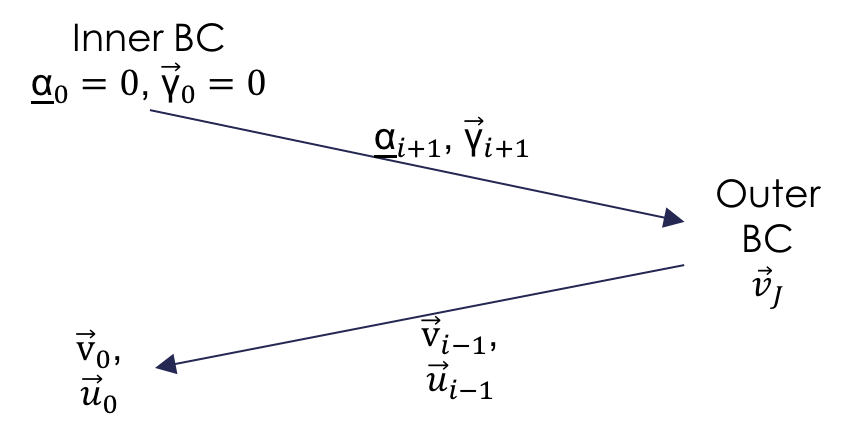
\includegraphics[width = 0.5 \textwidth]{figures/Overview.png}
\caption{A diagrammatic overview of the Henyey method, showing what is being evaluated at each stage of the code.}
\end{center}
\end{figure}







\subsection{$\underline{\alpha}$ and $\vec{\gamma}$ recurrence relations}

The relation $\vec{u} + \underline{\alpha} \vec{v} + \vec{\gamma} = 0$ is formulated this way as it enables the central boundary condition to be re-expressed as $\underline{\alpha} = 0$ and $\vec{\gamma} = 0$ at the centre.  By combining this initial condition with a recurrence relation, we can iterate outwards to find their values at all points in the star.

There are many different ways to formulate the recurrence relation, which will all be mathematically equivalent, although the particular form of the relations may have some computational effects, depending on how they are implemented.  The relevant equations are equations \ref{eq:relation}, \ref{eq:ACD} and \ref{eq:EFH}.  The key idea is to use these equations to reflect the structure of equation \ref{eq:relation}, evaluated at $k+1$, and to compare coefficients in order to get the equations for $\underline{\alpha}_{k+1}$ and $\vec{\gamma}_{k+1}$.

For ease of reading, the subscripts on the coefficients in equations \ref{eq:ACD} and \ref{eq:EFH} will be dropped, but the $k,k+1$ subscripts are implied, and any other subscripts will be explicitly stated.


Use equation \ref{eq:EFH} to substitute for $\vec{v}_{k}$ in equation \ref{eq:relation}.

\begin{equation} \label{eq:IIa}
\vec{v}_{k}  = \underline{F}^{-1}  \left( \vec{N} - \underline{E}  \vec{u}_{k}  - \underline{H} \vec{v}_{k+1} \right),
\end{equation}
\\
which leads to

\begin{equation} \label{eq:IIb}
 \underline{u}_{k}  + \underline{\alpha}_{k} \, \underline{F}^{-1} \left( \vec{N}  - \underline{E} \vec{u}_{k} - \underline{H} \vec{v}_{k+1}  \right)  +  \vec{\gamma}_{k}  =  0      \longrightarrow       \vec{u}_{k}  =  \left(  1 - \underline{\alpha}_{k} \, \underline{F}^{-1} \underline{E}  \right)^{-1}     \left(   \underline{\alpha}_{k} \, \underline{F}^{-1}  \left(  \underline{H}  \vec{v}_{k+1} - \vec{N} \right) - \vec{\gamma}_{k}  \right)
\end{equation} 
\\
which can be used to eliminate $\vec{u}_{k}$ in equation \ref{eq:ACD}, as

\begin{multline} \label{eq:IIc}
\vec{u}_{k+1}  + \underline{C}^{-1} \left(  \underline{D}  + \underline{A} \left( 1 - \underline{\alpha}_{k} \underline{F}^{-1} \underline{E}  \right)^{-1} \underline{\alpha}_{k} \underline{F}^{-1} \underline{H}    \right) \vec{v}_{k+1} \\
   -   \underline{C}^{-1} \left(  \vec{M}  +  \underline{A} \left( 1 - \underline{\alpha}_{k} \underline{F}^{-1} \underline{E}  \right)^{-1} \left(  \underline{\alpha}_{k} \underline{F}^{-1} \vec{N}  +  \vec{\gamma}_{k}   \right)  \right)   =  0
\end{multline} 
\\


This gives us the required recurrence relations as

\begin{equation} \label{eq:IIalpha}
\underline{\alpha}_{k+1}  =  \underline{C}^{-1} \left(  \underline{D}  + \underline{A} \left( 1 - \underline{\alpha}_{k} \underline{F}^{-1} \underline{E}  \right)^{-1} \underline{\alpha}_{k} \underline{F}^{-1} \underline{H}    \right) ,
\end{equation} 

\begin{equation} \label{eq:IIgamma}
\vec{\gamma}_{k+1}  =  -   \underline{C}^{-1} \left(  \vec{M}  +  \underline{A} \left( 1 - \underline{\alpha}_{k} \underline{F}^{-1} \underline{E}  \right)^{-1} \left(  \underline{\alpha}_{k} \underline{F}^{-1} \vec{N}  +  \vec{\gamma}_{k}   \right)  \right) .
\end{equation} 
\\







\subsection{Outer boundary}

In order to apply the outer boundary condition, it must be expressed in the similar terms to the discretised equations, that is, it must be formed as:

\begin{equation} \label{eq:OuterBC}
\underline{\eta} \, \vec{u}_{J-2} + \underline{\mu} \, \vec{u}_{J-1} + \underline{\nu} \, \vec{v}_{J-1} = \vec{x} .
\end{equation}
\\
This condition is actually evaluated at the centre of the outer-most cell, and although that it not strictly the outermost part of the star, it is as far out as you can go without having to extrapolate.

In order to get values for $\vec{u}_{J-1}$ and $\vec{v}_{J-1}$, we must combine equation \ref{eq:OuterBC} with equations \ref{eq:ACD}, \ref{eq:EFH} and \ref{eq:relation}, all evaluated for $k = J-2$.  This gives us four equations for four unknowns, which is a closed set of independent equations, so can be solved.

Multiply equation \ref{eq:EFH} by $\underline{\alpha}_{J-2} \underline{F}^{-1}$ from the left, and use equation \ref{eq:relation} to eliminate $\underline{\alpha}_{J-2} \vec{v}_{J-2}$, giving

\begin{equation} \label{eq:BCa}
\underline{\alpha}_{J-2} \underline{F}^{-1} \underline{E} \vec{u}_{J-2}  -  \vec{u}_{J-2}  -  \vec{\gamma}_{J-2}  +  \underline{\alpha}_{J-2} \underline{F}^{-1} \underline{H} \vec{v}_{J-1}  =  \underline{\alpha}_{J-2} \underline{F}^{-1} \vec{N}
\end{equation} 
\\

which can be rearranged to give an expression for $\vec{u}_{J-2}$


\begin{multline} \label{eq:BCa}
\left(  \underline{\alpha}_{J-2} \underline{F}^{-1} \underline{E}  -  1  \right)  \vec{u}_{J-2}   +  \underline{\alpha}_{J-2} \underline{F}^{-1} \underline{H} \vec{v}_{J-1}  =  \underline{\alpha}_{J-2} \underline{F}^{-1} \vec{N}  +  \vec{\gamma}_{J-2} 
\\ \longrightarrow
\vec{u}_{J-2} = \left(  \underline{\alpha}_{J-2} \underline{F}^{-1} \underline{E}  -  1  \right)^{-1}   \left(  \underline{\alpha}_{J-2} \underline{F}^{-1} \vec{N}  +  \vec{\gamma}_{J-2}  -   \underline{\alpha}_{J-2} \underline{F}^{-1} \underline{H} \vec{v}_{J-1}  \right)
\end{multline} 
\\

This enables $\vec{u}_{J-2}$ to be eliminated, but, for simplicity, we first eliminate $\vec{u}_{J-1}$ from equations \ref{eq:OuterBC} and \ref{eq:ACD}.

Multiply equation \ref{eq:OuterBC} by $\underline{\mu}^{-1}$, and equation \ref{eq:ACD} by $\underline{C}^{-1}$, giving

\begin{equation} \label{eq:BCb}
\underline{\mu}^{-1}  \underline{\eta} \, \vec{u}_{J-2} + \vec{u}_{J-1} + \underline{\mu}^{-1}  \underline{\nu} \, \vec{v}_{J-1} =  \underline{\mu}^{-1} \vec{x}
\end{equation}

\begin{equation} \label{eq:BCc}
\underline{C}^{-1}  \underline{A} \vec{u}_{J-2}  +  \vec{u}_{J-1}  +  \underline{C}^{-1} \underline{D} \vec{v}_{J-1}  =  \underline{C}^{-1}  \vec{M} .
\end{equation}
\\

Taking the difference of these equations allows us to get an expression for $\vec{v}_{J-1}$ in terms of $\vec{u}_{J-2}$, as

\begin{equation} \label{eq:BCd}
\left(  \underline{\mu}^{-1}  \underline{\eta}   -  \underline{C}^{-1}  \underline{A}  \right) \vec{u}_{J-2}  +  \left(  \underline{\mu}^{-1}  \underline{\nu}   -  \underline{C}^{-1} \underline{D} \right)  \vec{v}_{J-1}  =  \underline{\mu}^{-1} \vec{x}  -  \underline{C}^{-1}  \vec{M} 
\end{equation}
\\

which gives, when equation \ref{eq:BCa} is used to substitute an expression for $\vec{u}_{J-2}$:

\begin{multline} \label{eq:BCe}
\left(  \underline{\mu}^{-1}  \underline{\eta}   -  \underline{C}^{-1}  \underline{A}  \right) \left(  \underline{\alpha}_{J-2} \underline{F}^{-1} \underline{E}  -  1  \right)^{-1}   \left(  \underline{\alpha}_{J-2} \underline{F}^{-1} \vec{N}  +  \vec{\gamma}_{J-2}  -   \underline{\alpha}_{J-2} \underline{F}^{-1} \underline{H} \vec{v}_{J-1}  \right)  \\
+  \left(  \underline{\mu}^{-1}  \underline{\nu}   -  \underline{C}^{-1} \underline{D} \right)  \vec{v}_{J-1}  =  \underline{\mu}^{-1} \vec{x}  -  \underline{C}^{-1}  \vec{M}   .
\end{multline}
\\

This can then be rearranged for an expression for $\vec{v}_{J-1}$ as

\begin{multline} \label{eq:v_J-1_long}
\vec{v}_{J-1}  =   \left(    \underline{\mu}^{-1} \underline{\nu}   - \underline{C}^{-1} \underline{D}  +  \left(   \underline{\mu}^{-1} \underline{\eta}  - \underline{C}^{-1} \underline{A}  \right)  \left(   1  - \underline{\alpha}_{J-2} \underline{F}^{-1} \underline{E}  \right)^{-1} \underline{\alpha}_{J-2}  \underline{F}^{-1} \underline{H}  \right)^{-1}    \\
\left(   \underline{\mu}^{-1} \vec{x}  -  \underline{C}^{-1} \vec{M}  +   \left(   \underline{\mu}^{-1} \underline{\eta}  - \underline{C}^{-1} \underline{A}  \right)  \left(   1  - \underline{\alpha}_{J-2} \underline{F}^{-1} \underline{E}  \right)^{-1}   \left(    \vec{\gamma}_{J-2}  +  \underline{\alpha}_{J-2} \underline{F}^{-1}  \vec{N}   \right)  \right)  .
\end{multline}
\\
This can be simplified further by using expressions for $\underline{\alpha}_{J-1}$ and $\vec{\gamma}_{J-1}$, and by using the expression $\underline{\mu}^{-1} \underline{\mu} = 1$ to give:

\begin{equation} \label{eq:v_J-1}
\vec{v}_{J-1}  =   \left(    \underline{\nu}   -  \underline{\mu} \, \underline{\alpha}_{J-1}  +  \underline{\eta} \, \underline{A}^{-1} \left( \underline{C} \, \underline{\alpha}_{J-1}  -  \underline{D} \right)  \right)^{-1}    
\left(   \vec{x}  +  \underline{\mu} \, \vec{\gamma}_{J-1}  -   \underline{\eta} \, \underline{A}^{-1} \left(   \underline{C} \vec{\gamma}_{J-1} - \vec{M}   \right)  \right)  .
\end{equation}
\\








\subsection{$\vec{u}_{k-1}$ and $\vec{v}_{k-1}$ recurrence relation}

At this point, $\underline{\alpha}_{k}$ and $\vec{\gamma}_{k}$ are known at all points, and both $\vec{u}_{J-1}$ and $\vec{v}_{J-1}$ are known.  In order to find the solution at all points in the star, a recurrence relation must be found in order to express $\vec{u}_{k}$ or $\vec{v}_{k}$ in terms of $\vec{u}_{k+1}$ and $\vec{v}_{k+1}$.  This doesn't match the title of the section, but that is just a simple shift in dummy variable to match my previous working, and to make it so that the implied subscripts of $k,k+1$ are still valid.

There are two ways to go about this, which is essentially a choice of which equation to use: equation \ref{eq:ACD} or \ref{eq:EFH}.

\subsubsection{Case I}

Because of previous choices, Case I uses equation \ref{eq:EFH}.  We substitute for $\vec{u}_{k}$ using equation \ref{eq:relation}, and rearrange for $\vec{v}_{k}$.

\begin{equation} \label{eq:Case_I}
- \underline{E} \, \underline{\alpha}_{k} \vec{v}_{k}  -  \underline{E} \vec{\gamma}_{k} + \underline{F} \vec{v}_{k} + \underline{H} \vec{v}_{k+1} = \vec{N}
\longrightarrow   \vec{v}_{k}  =  \left(  \underline{F}  -  \underline{E} \, \underline{\alpha}_{k}  \right)^{-1}  \left(  \vec{N}  +  \underline{E} \vec{\gamma}_{k}  -  \underline{H} \vec{v}_{k+1} \right)
\end{equation} 
\\



\subsubsection{Case II}

Case II uses equation \ref{eq:ACD}.  This rearrangement is pretty simple, and gives us:

\begin{equation} \label{eq:Case_II}
\vec{u}_{k}  =  \underline{A}^{-1}  \left(  \vec{M}  -  \underline{C} \vec{u}_{k+1}  -  \underline{D} \vec{v}_{k+1} \right)
\end{equation} 
\\









\subsection{Practicalities}

This section is largely comprised of problems which I have overcome in the making of this code, from improvements to reduce discretisation effects, to better ways to use memory effectively.





\subsubsection{Memory}

A naive approach might be to define $J \times 2 \times 2$ arrays for each matrix and vector, which would lead to at least $38 x J$ doubles in the memory (double that if complex numbers must be used).  This neglects the significant memory usage required by the input data, and also neglects the necessary dummy variable matrices which would be needed to manipulate these basic matrices to implement the necessary relations without causing horrendous confusion along the way.

In order to reduce the memory usage, it is necessary to realise exactly which arrays must be saved over the whole star, and to cut down the size of those that needn't be.  Obviously $\underline{\alpha}_{k}$ and $\vec{\gamma}_{k}$ must span the entire star, as must $\vec{u}_{k}$ and $\vec{v}_{k}$.  Somewhat more subtly, however, there must be some arrays which remember something about zone $k-1$ on the way back from the surface in order to iterate for $\vec{u}_{k-1}$ or $\vec{v}_{k-1}$.  These expressions for these recursive arrays are found in equations \ref{eq:Case_I} and \ref{eq:Case_II}, depending on which case you chose to use.

They are defined as

\begin{equation} \label{eq:REC_def}
\vec{f}_{k}  =  \underline{RECu}_{k} \vec{u}_{k+1}  +  \underline{RECv}_{k} \vec{v}_{k+1}  +  \vec{RECc}_{k}
\end{equation}
\\
where $\vec{f}_{k}$ is a stand-in for either $\vec{u}_{k}$ or $\vec{v}_{k}$ depending on the case used.  Because of this, we only require 4 matrices and 3 vectors to be saved over the whole star ($\underline{\alpha}$, $\underline{RECu}$, $\underline{RECv}$, $\vec{RECc}$, $\vec{\gamma}$, $\vec{u}$, $\vec{v}$), and the other vector and matrix arrays need only be $1 \times 1 \times 2$ and $1 \times 2 \times 2$ respectively -- this is because we need only know the $k$ arrays at any one time, so we define only that array and redefine it when we move to the $k+1$ cell.

In order to do this effectively, all of the matrix manipulations from the definitions of matrices $\underline{A}$ to $\underline{H}$ to the definitions of $\underline{\alpha}_{k}$, $\vec{\gamma}$ and the recurrence arrays ($\underline{RECu}$, $\underline{RECv}$ and $\vec{RECc}$) must be done within the same for loop.





\subsubsection{Averaging in equation \ref{eq:EFH}}

This is a fairly simple note, which essentially points out that the location at which this equation is valid is at the outer edge of zone $k$, which is not generally halfway between the midpoints of zones $k$ and $k+1$.  In order to accurately interpolate to find the values of quantities evaluated at cell midpoints we must use a weighted average.

\begin{equation} \label{eq:weighted_average}
\bar{q}  =  \Delta_{k} q_{k}  +  \Delta_{k+1} q_{k+1}
\end{equation}
\\
where $q$ is some input variable which is given at the cell centres, $\bar{q}$ is the value of $q$ at the outer edge of cell $k$, and where the weightings are

\begin{equation} \label{eq:delta_k}
\Delta_{k} =  \frac{r^{mid}_{k+1} - r^{b}_{k}}{r^{mid}_{k+1} - r^{mid}_{k}}
\end{equation}

\begin{equation} \label{eq:delta_k+1}
\Delta_{k+1} =  \frac{r^{b}_{k} - r^{mid}_{k}}{r^{mid}_{k+1} - r^{mid}_{k}}
\end{equation}
\\
and $r^{b}_{k}$ is the radius at the outer boundary of cell $k$, and $r^{mid}_{k}$ is the radius at the centre of cell $k$.















\end{document}  
